\documentclass{./public/ufpatcc}


\usepackage{multirow}
\usepackage{graphicx}
\usepackage{url}
\usepackage{amsmath,amssymb}
\usepackage[brazil]{babel}
\usepackage[utf8]{inputenc} 	
\usepackage{appendix}
\usepackage{graphicx,color,amsmath,cite,url,amssymb,subfigure}
\usepackage{multirow} %tables with multiple rows
\usepackage{listings} % to list source code: http://www.usq.edu.au/users/leis/notes/latex/code.html
\usepackage{ifpdf} 



\usepackage{multirow}
\usepackage{graphicx}
\usepackage{url}
\usepackage{amsmath,amssymb}

\usepackage[brazil]{babel}
%\usepackage[latin1]{inputenc}	%For Windows users
\usepackage[utf8]{inputenc} 		%For Linux users
%incluir tudo no table of contents
    \setcounter{secnumdepth}{5}
    \setcounter{tocdepth}{5}
%exemplos de como ensinar o latex a separar silabas corretamente
\hyphenation {mo-de-lo}
\hyphenation {EXCELENTE}
\hyphenation {bra-si-lei-ros}
\hyphenation {a-mos-tras}
\hyphenation {SEMINF}
\hyphenation {re-co-nhe-ci-men-to}
\hyphenation {apre-sen-tan-do}
\hyphenation {cor-res-pon-den-tes}
\hyphenation {mo-de-los}
\hyphenation {pro-ba-bi-li-da-de}
\hyphenation {co-nhe-ci-do}
\hyphenation {li-ne-ar}
\hyphenation {co-nhe-ci-men-to}
\hyphenation {di-fe-ren-tes}
\hyphenation {as-cen-den-tes}
\hyphenation {ade-qua-da-men-te}
\hyphenation {com-par-ti-lham}
\hyphenation {apre-sen-ta}
\hyphenation {ge-ra-da}
\hyphenation {res-pec-ti-va-men-te}
\hyphenation {re-co-nhe-ci-men-to}
\hyphenation {software}
\hyphenation {de-ta-lha-da-men-te}
\hyphenation {des-cen-den-tes}
\hyphenation {des-cri-tos}
\hyphenation {li-ne-a-res}
\hyphenation {ufpaspeech}
\hyphenation {re-co-nhe-ce-dor}

\usepackage{appendix}

%To use Portuguese:
%\usepackage[brazil]{babel}   % Para hifenar em portugues
%\usepackage[latin1]{inputenc}% Para poder digitar os acentos da maneira usual:
%\usepackage[utf8]{inputenc} %Mesmo acima, mas pra Linux

%\usepackage{ucs} %Unicode functionality

%\usepackage{mathrsfs} %math alphabet I will use for sets
%%\usepackage{ascii}
%%\usepackage{mathabx} %convolution symbol
%\usepackage{makeidx}  %to generate indices, I guess
%\usepackage{graphicx,color,amsmath,cite,url,amssymb,subfigure}
%\usepackage{multirow} %tables with multiple rows
%%\usepackage{pslatex}	% to use PostScript fonts instead of Computer Modern. AK: not sure if I liked
\usepackage{color}
\definecolor{light-gray}{gray}{0.95}
\usepackage{listings} % to list source code: http://www.usq.edu.au/users/leis/notes/latex/code.html
\lstset{language=Java}
\lstset{backgroundcolor=\color{light-gray}}
%\lstset{linewidth=90mm}
%By default, keywords are typeset bold, comments in italic shape, and spaces in strings appear
%as . You dont like these settings? Look at this:
\lstset{% general command to set parameter(s)
commentstyle=\color{blue}, % white comments
stringstyle=\ttfamily, % typewriter type for strings
showstringspaces=false, % no special string spaces
identifierstyle=, % nothing happens
keywordstyle=, % nothing happens
keywordstyle=\color{red}\bfseries ,
linewidth=\textwidth} %framed box is the text size
%\lstset{frame=lines}
%\lstset{frameround=tttt}
%\lstset{frameround=trbl}  %frameround is not working. use frame:
\lstset{frame=trbl}
%\lstset{labelstep=1}
\lstset{basicstyle=\small} % print whole listing small
\lstset{firstnumber=1, numberfirstline=false, numbers=left, numberstyle=\tiny, stepnumber=5, numbersep=5pt} %add line numbering
%The key nolol suppresses an entry for both the environment or the input command.

\usepackage{ifpdf} %The package provides the switch \ifpdf:
%Example of usage:
%\ifpdf
%. . . do things, if pdfTEX is running in pdf mode . . .
%\else
%. . . other TEX like latex or pdfTEX in dvi mode . . .
%\fi

%NF: including hyperlinks and thumbnails features
\ifpdf
	\usepackage[pdftex,colorlinks]{hyperref}
	\usepackage[pdftex]{thumbpdf} %% in case of pdfLaTeX
	\usepackage{pdflscape}
%Latex pitfalls: when using dvips the figures must be .eps and
%when using pdftex the figures must be .pdf (pdftex does not accept .eps)
%To learn about the issue, read:
%http://www.math.rug.nl/~trentelman/jacob/pdflatex/pdflatex.html
%http://www.latex-community.org/viewtopic.php?p=1182
%http://mintaka.sdsu.edu/GF/bibliog/latex/LaTeXtoPDF.html
%I (Aldebaro) added the package below:
\usepackage{epstopdf}
%and also used Alt+F7 in TeXnicCenter to include --enable-write18 in the command line that invokes 
%the pdftex "compiler". The warning is still there, but the eps => pdf figure conversion now is
%done on-the-fly. Later we will have to learn how to use \ifpdf to make the .tex compatible with both
%latex and pdftex. For that, read: http://www.math.rug.nl/~trentelman/jacob/pdflatex/pdflatex.html
%command to pdftex:
%To choose how the system is opened:
%pdfstartview={FitH}
%Possible values are:
%"Fit", to show the whole page;
%"FitH", to show the width of the page in the window;
%or "FitB", the width of the contents to the window.
\hypersetup{%
pdftitle={Realidade Virtual e Equações de Maxwell},
pdfauthor={Paulo Victor Mocbel dos Santos},
pdfkeywords={ASR, SpeechOO, Acessibilidade},
pdfstartview={FitH}, %% <--
urlcolor=black,
linkcolor=black,
citecolor=black,
}
\fi

\graphicspath{{./figures/}}
\linespread{1.5}

\sloppy

\ufpaTitulo{Realidade Virtual e Solução Numérica das Equações de Maxwell}
\ufpaAutor{Paulo Victor Mocbel dos Santos}
\ufpaOrientador{Prof. Dr. Rodrigo Melo e Silva de Oliveira }
\ufpaCoOrientador{Washington César Braga de Sousa}
\ufpaMembroBancaA{Prof. Dr. Felipe}
\ufpaMembroBancaB{Prof. Dr. Josivaldo}
\ufpaCoordenadorCurso{Prof. Dr. Ádamo Lima de Santana}


\begin{document}


\begin{ufpaEpigrafe}
A adversidade leva alguns a serem vencidos e
 outros a baterem recordes. William Arthur Ward
\end{ufpaEpigrafe}

\ufpaPaginaDeAprovacao

%%%%%%%%%%%%%%%%%%%%%%%%%%%%%%%%%%%
% Oferecimento
%%%%%%%%%%%%%%%%%%%%%%%%%%%%%%%%%%%
\begin{ufpaOferecimento}
    \index{Oferecimento@Oferecimento}%
    \addcontentsline{toc}{chapter}{Dedicatria}
    Dedico esse TCC a minha famlia e amigos, pelo apoio e incentivo,
    sem os quais, este trabalho no seria possvel.
\end{ufpaOferecimento}

%%%%%%%%%%%%%%%%%%%%%%%%%%%%%%%%%%%
% Agradecimento
%%%%%%%%%%%%%%%%%%%%%%%%%%%%%%%%%%%
\begin{ufpaAgradecimentos}
    \index{Agradecimentos@Agradecimentos}%
    \addcontentsline{toc}{chapter}{Agradecimentos}

		Dedico esse trabalho a minha familia que sempre me apoio. Agradeço a todos os meus amigos e colegas de turma, por terem me ajudado nessa caminhada.

    \begin{flushright}
        Paulo Victor Mocbel dos Santos
    \end{flushright}

\end{ufpaAgradecimentos}

%%%%%%%%%%%%%%%%%%%%%%%%%%%%%%%%%%%
% Sumário
%%%%%%%%%%%%%%%%%%%%%%%%%%%%%%%%%%%
\tableofcontents    \clearpage

%%%%%%%%%%%%%%%%%%%%%%%%%%%%%%%%%%%
% Lista de figuras e lista de tabelas
%%%%%%%%%%%%%%%%%%%%%%%%%%%%%%%%%%%
\listoffigures \clearpage \listoftables \clearpage

% Lista de siglas
\chapter*{Lista de Abreviaturas}
\addcontentsline{toc}{chapter}{Lista de Abreviaturas}

\begin{description}
	\item[$\overline{E}$]	Vetor intensidade de campo elétrico ($V/m$)
	\item[$\overline{H}$]	Vetor intensidade do campo magnético ($A/m$)
	\item[$\epsilon$]	Permissividade elétrica ($farad/m$)
	\item[$\mu$]	Permeabilidade magnética ($henry/m$)
	\item[$\sigma$]	Condutividade elétrica ($siemen/m$)
	\item[2D]	Bidimensional 
	\item[3D]	Tridimensional 
	\item[FDTD]	Finite-difference time-domain 
	\item[B-rep ou BREP]	Boundary Representation 
	\item[RV]	Realidade Virtual 
	\item[AV]	Ambiente Virtual 
	\item[LANE-SAGS]	Synthesis and Analysis of Grounding Systems 
\end{description}

\clearpage

\begin{ufpaResumo}
Neste trabalho, foi realizado o estudo de propagação de ondas eletromagnáticas em um ambiente \textit{indoor}. Estudo esse efetuado através do desenvolvimento de uma interface que modela cenários 3D. Por meio da qual pode-se obeter uma malha compatível com o simulador que usa o método FDTD (LANE-SAGS). Com essa malha, foram feitas várias simulações, cada uma delas referente a um posicionamento diferente da antena nesse ambiente, sempre comparando as repostas simuladas com os valores esperimentais.
\end{ufpaResumo}

%%%%%%%%%%%%%%%%%%%%%%%%%%%%%%%%%%%
% Corpo do tcc
%%%%%%%%%%%%%%%%%%%%%%%%%%%%%%%%%%%
\pagenumbering{arabic}

\chapter{Introdução}
	Com o passar dos anos, a computação tem evoluído de forma exponencial\cite{comp_history}, permitindo cada vez mais ao ser humano: armazenar grande quantidades de dados, simular ambientes de grandes magnitudes, fazer previsão de eventos, se comunicar audiovisualmente, etc. Todo esse avanço vem refletindo de forma crescente na vida do homem.

	Mais especificamente na área de telecomunicações, pode-se dizer que esse crescimento vem possibilitando avanços nos estudos e aplicações relacionadas às simulações de ondas eletromagnéticas e antenas. O método das Diferenças Finitas no Domínio do Tempo (FDTD)\cite{fdtd_intro} é um dos mais usados (e antigos) nos estudos relativos à propagações de ondas eletromagnéticas em ambientes \textit{indoor} e \textit{outdoor}\cite{rodrigo_intro}.

	Porém, muitas vezes, a representação virtual de desses ambientes não é uma tarefa fácil. Dessa forma, surge a necessidade de criação de \textit{softwares} que auxiliem nessa construção. Eles podem ser de modelagem 2D ou 3D desde de que permitam a criação de estruturas básicas, como: triângulos, círculos, cubos, esferas e pirâmides; como também outras bem mais complexas(fractais, estruturas periódicas e prédios), gerando sempre a base que contenha as coordenadas de cada objeto desse cenário.

\section{Objetivos}
	Esse trabalho tem com finalidade a construção de um \textit{software} que permita modelar ambientes tridimensionais (usando conceitos de realidade virtual) que se aproximem, da melhor forma possível, um cenário real. A partir desse universo virtual, objetiva-se obter a malha compatível com o programa LANE-SAGS. Através dele, simular a propagação de ondas eletromagnéticas utilizando o método FDTD. Assim possibilitando analisar tanto aterramento e descargas elétricas quanto a resposta desse cenário a propagação do sinal de uma antena.

	Dessa forma, os principais objetivos desse trabalho são:
\begin{enumerate}
\item {Representar estruturas tridimensionais por meio de alguns objetos básicos, como: cubo, esfera, cilindro e cone.}
\item {Criar AV com base em ambientes reais. }
\item {Gerar uma base de dados com as característica de cada estrutura, sua posição, dimensão e parâmetros físicos($\mu$, $\sigma$ e $\epsilon$).}
\item {Gerar malha compatível com o simulador LANE-SAGS, efetuar a simulação e comparar os resultados com experimentos reais relativos à propagação eletromagnética em um ambiente \textit{indoor}.}
\end{enumerate}

\section{Organização do Trabalho}
	Este trabalho foi estruturado da seguinte forma:
\begin{itemize}
\item \textbf{Capítulo 2:} Trata da base teórica necessária para realização do trabalho, falando de computação gráfica, técnicas de modelagem de sólidos, teoria dos grafos de cena e o método FDTD.
\item \textbf{Capítulo 3:} Fala sobre a interface desenvolvida nesse trabalho, suas aplicações, classes, aparência, objetos básicos, manipuladores de cena, região de análise e seus parâmetros, geração de malha, posicionamento de câmera, atalhos de teclado, eventos de mouse, etc. 
\item \textbf{Capítulo 4:} Mostra uma aplicação usando o \textit{software} com seus resultados (comparados com os obtidos via medição), seguindo todos os passos desde da criação de um ambiente até sua simulação no LANE-SAGS.
\end{itemize}


\chapter{Fundamentação Teórica}
\section{Computação Gráfica e Modelagem 3D}
A computação gráfica esta presente em quase tudo na vida do homem, desde de pequenos jogos para celular até projetos grandiosos para viagens espaciais, tendo também um papel fundamental na medicina, onde possibilita a visualizações de órgãos internos ao corpo humano o que vem ajudando no tratamento de várias doenças\cite{comp_grafica_h}\cite{azevedo}\cite{kirne}. Esta presente também em muitos outros segmentos, tais como os descritos na tabela~\ref{tab:comp_teoria}. \\

\begin{table}
\centering
\begin{tabular}{|l|l|}
	\hline
	Área & Aplicações \\ \hline
	Medicina &  Exames, diagnósticos, estudo, planejamento de procedimentos\\ \hline
	Arquitetura & Perspectivas, projetos de interiores e paisagismo\\ \hline
	Engenharia & Em todas as suas áreas (mecânica, civil, aeronáutica etc.)\\ \hline
	Meteorologia & Previsão do tempo, reconhecimento de poluição\\ \hline
	Segurança Pública & Definição de estratégias, treinamento, reconhecimento\\ \hline
	Astronomia & Tratamento de imagens, modelagem de superfícies\\ \hline
	Artes & Efeitos especiais, modelagens criativas, esculturas e pinturas\\
	\hline
\end{tabular}
\caption{Diferentes ramos da computação gráfica.}
\label{tab:comp_teoria}
\end{table}

Um dos pioneiros no quesito computação gráfica foi o aluno do MIT\footnote{MIT - Massachusetts Institute of Technology}, Ivan Sutherland, que criou um programa de desenho chamado Sketchpad\cite{sutherland}. Através de uma caneta a laser, podia-se desenha na tela de um computador, salvar e depois recarregar o desenho feito.\\

 Mais o primeiro computador com recursos gráficos de visualização de dados numéricos foi o \textbf{Whirlwind I}, também desenvolvido pelo \textbf{MIT}. As industrias automobilística e aeroespacial começaram a utilizá-lo , e assim esse, até então, novo campo da computação foi se desenvolvendo, abrangendo outros segmentos de atuação e com isso melhorando de forma exorbitante\cite{comp_grafica_h2}.  \\

\subsection{Sistemas de Coordenadas}
Um sistema de coordenada é aquele que se utiliza para descrever objetos modelados em um universo. Através dele, consegue-se capturar, por exemplo, a posição e as dimensões dos objetos. Existem vários sistemas, a Figura~\ref{fg:coordenadas} mostra três deles, que são: coordenadas polares, esféricas e cilíndricas. Onde o primeiro, através do raio e um ângulo podemos chegar a qualquer coordenada. Já para o segundo, obtemos as coordenadas pelo raio e dois ângulos. No terceiro, consegue-se um ponto qualquer na região de análise através do raio, um ângulo e um comprimento.\\ 

\begin{figure}[ht!]
	\centering
	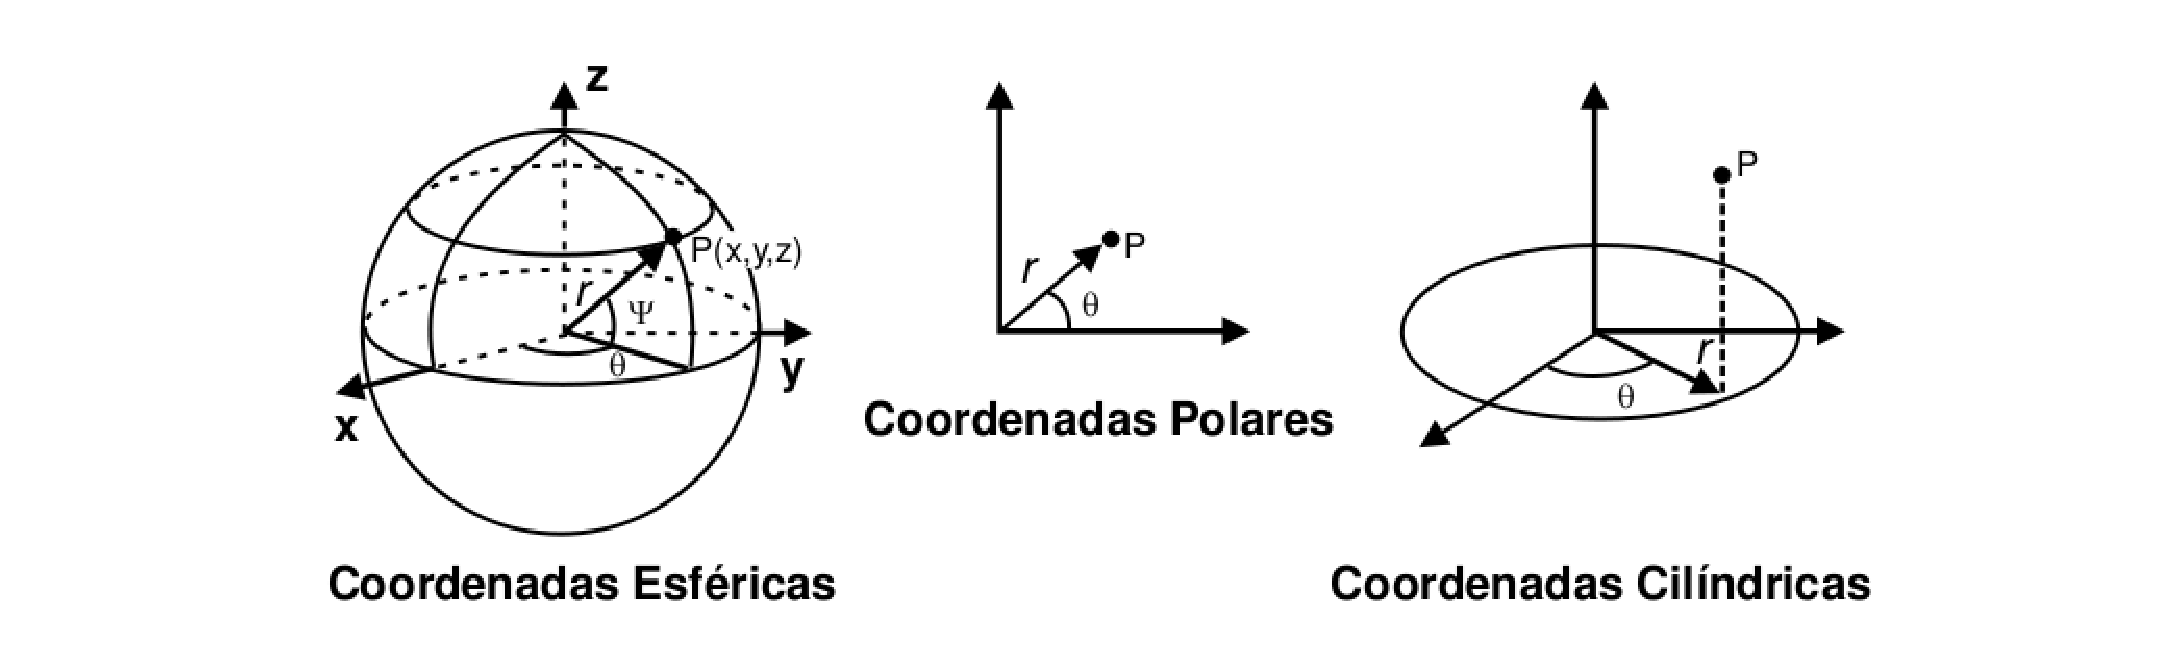
\includegraphics[scale=0.4]{s_coordenadas}
	\caption{Sistemas de coordenadas.}
	\label{fg:coordenadas}
\end{figure}

\subsection{Transformações}
As transformações são umas das características mais importantes da computação gráfica. Elas representam um mapeamento de ponto(s) de uma determinada posição para outra~\cite{comp_grafica1}. As transformações mais usadas e conhecidas são: rotação, escala e translação.\\

%--------------tranlasao---------------
Transladar significa mover o objeto. Essa operação é dada pela equação~\ref{eq:translacao}, onde adicionando quantias($T_x$, $T_y$ e $T_z$) a sua coordenada atual($x$, $y$ e $z$), obtém-se uma nova posição, transladada($x'$, $y'$ e $z'$). A Figura~\ref{fg:trans} mostra essa transformação. \\

\begin{equation}\label{eq:translacao}
[x'\ y'\ z'] = [x\ y\ z] + [T_{x}\ T_{y}\ T_{z}]
\end{equation}

\begin{figure}[ht!]
      \centering
	  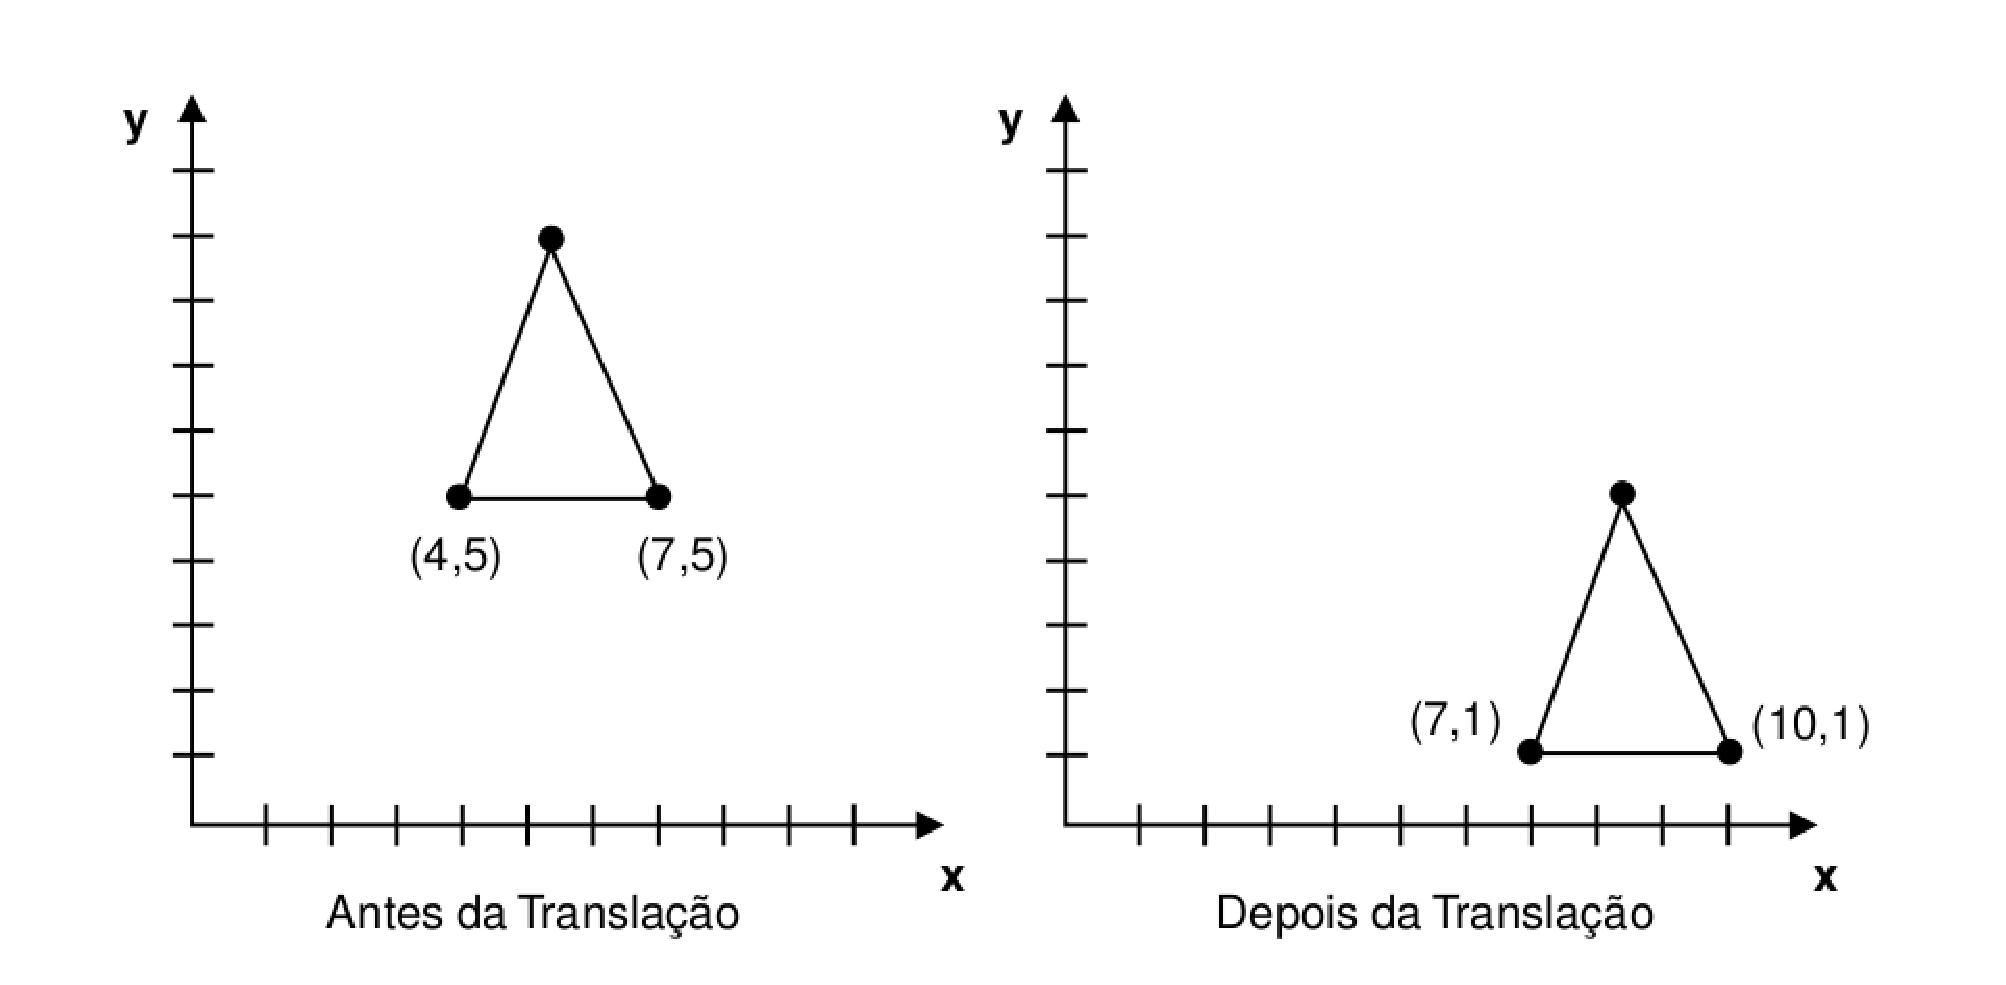
\includegraphics[scale=0.4]{trans}
	  \caption{Operação de Translação 2D.}
	  \label{fg:trans}
\end{figure} 

%--------------escala---------------
A operação de escala é aquela associada à mudança de dimensão dos objetos. Ela é representada pela equação matricial~\ref{eq:escala}, que mostra que quando multiplicamos as dimensões atuais ($x$, $y$ e $z$) por alguns fatores ($S_x$, $S_y$ e $S_z$), obtemos um novo objeto escalado ($x'$, $y'$ e $z'$). A Figura~\ref{fg:escala} mostra bem o que ocorre quando escalonamos um objeto.\\

\begin{equation}\label{eq:escala}
    \begin{array}{c c c}
    [x' \ y' \ z'] = [x \ y \ z]
    \begin{bmatrix}
     S_x & 0 & 0   \\[0.2em]
     0 & S_y & 0   \\[0.2em]
     0 & 0 & S_z
    \end{bmatrix}
    \
    = [xS_x\ yS_y\ zS_z]
    \end{array}
\end{equation}

\begin{figure}[ht!]
      \centering
	  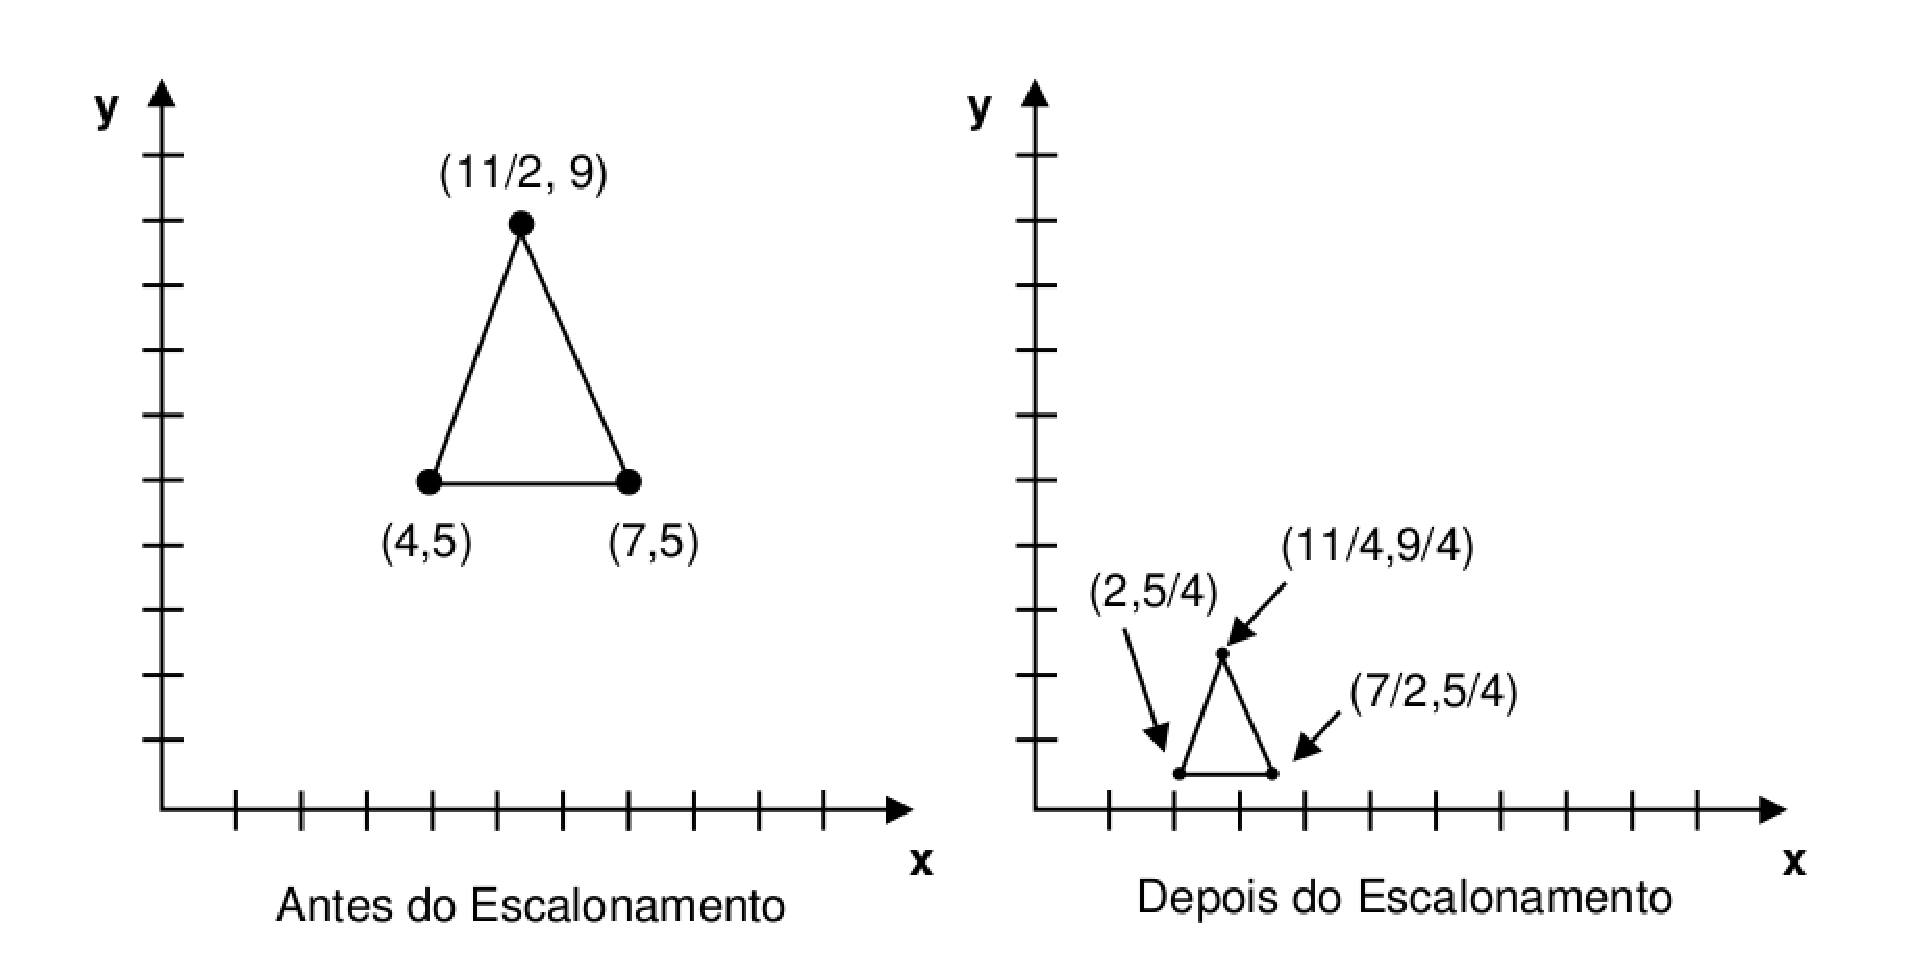
\includegraphics[scale=0.4]{escala}
	  \caption{Operação de Escala 2D.}
	  \label{fg:escala}
\end{figure} 

%--------------rotacao---------------
Por fim, quando desejamos girar um objeto ou um ponto no nosso sistema de coordenadas, usamos a transformação de rotação, a qual pode ser representada pelas formas matriciais~\ref{eq:rotacao}, que mostram, respectivamente, as matrizes rotação para os eixos $x$, $y$ e $z$. A Figura~\ref{fg:rotacao}, ilustra essa operação.

\begin{figure}[ht!]
      \centering
	  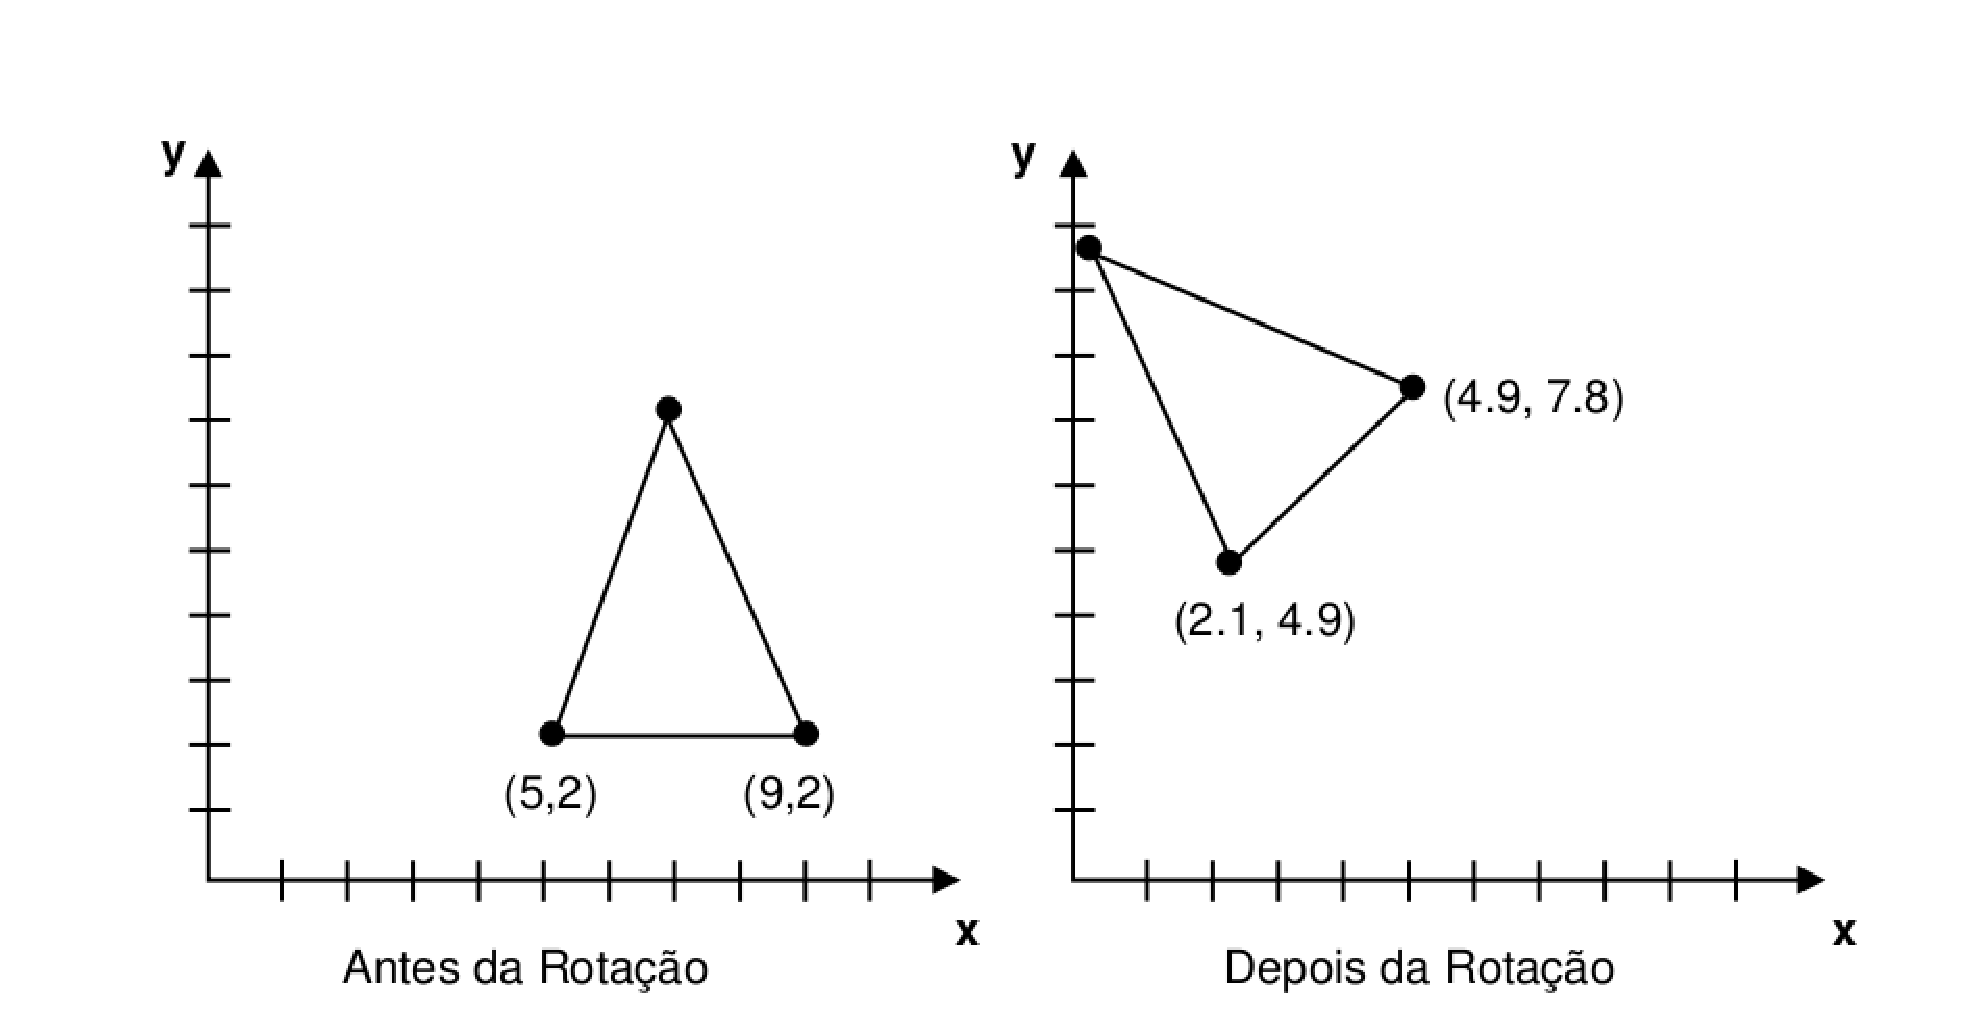
\includegraphics[scale=0.4]{rotacao}
	  \caption{Operação de Rotação 2D.}
	  \label{fg:rotacao}
\end{figure} 
\begin{center}
\begin{equation}\label{eq:rotacao}
  \begin{array}{c c c}
     R_x(\theta) = \begin{bmatrix}
    1 & 0 & 0   \\[0.2em]
    0 & \cos(\theta) & -\sin(\theta)    \\[0.2em]
    0 & \sin(\theta) & \cos(\theta) \\
    \end{bmatrix}
    , 
    R_y(\theta) = \begin{bmatrix}
    \cos(\theta) & 0 & \sin(\theta) \\[0.2em]
    0 & 1 & 0   \\[0.2em]
    -\sin(\theta) & 0 & \cos(\theta)\\
    \end{bmatrix}
    ,
    R_z(\theta) = \begin{bmatrix}
    \cos(\theta) & -\sin(\theta) & 0\\[0.2em]
    \sin(\theta) & \cos(\theta) & 0\\[0.2em]
    0 & 0 & 1\\\ 
    \end{bmatrix}
    \end{array}
\end{equation}
\end{center}

\subsection{Representação de Sólidos}
\subsubsection{Representação Armada ou Wireframe}
É a representação dada por um conjunto de arrestas que define as bordas do objeto\cite{speck}. Tem a vantagem de ser mais rápida quanto a renderização, porém tem um problema relacionado ao fato de dar margem para várias interpretações, além de dificultar cálculos como: volume e massa de sólidos. Por isso, ela geralmente não é considerada uma técnica de modelagem de sólidos. A Figura~\ref{fg:wireframe} esta ilustrando essa técnica.

\begin{figure}[ht!]
	\centering
	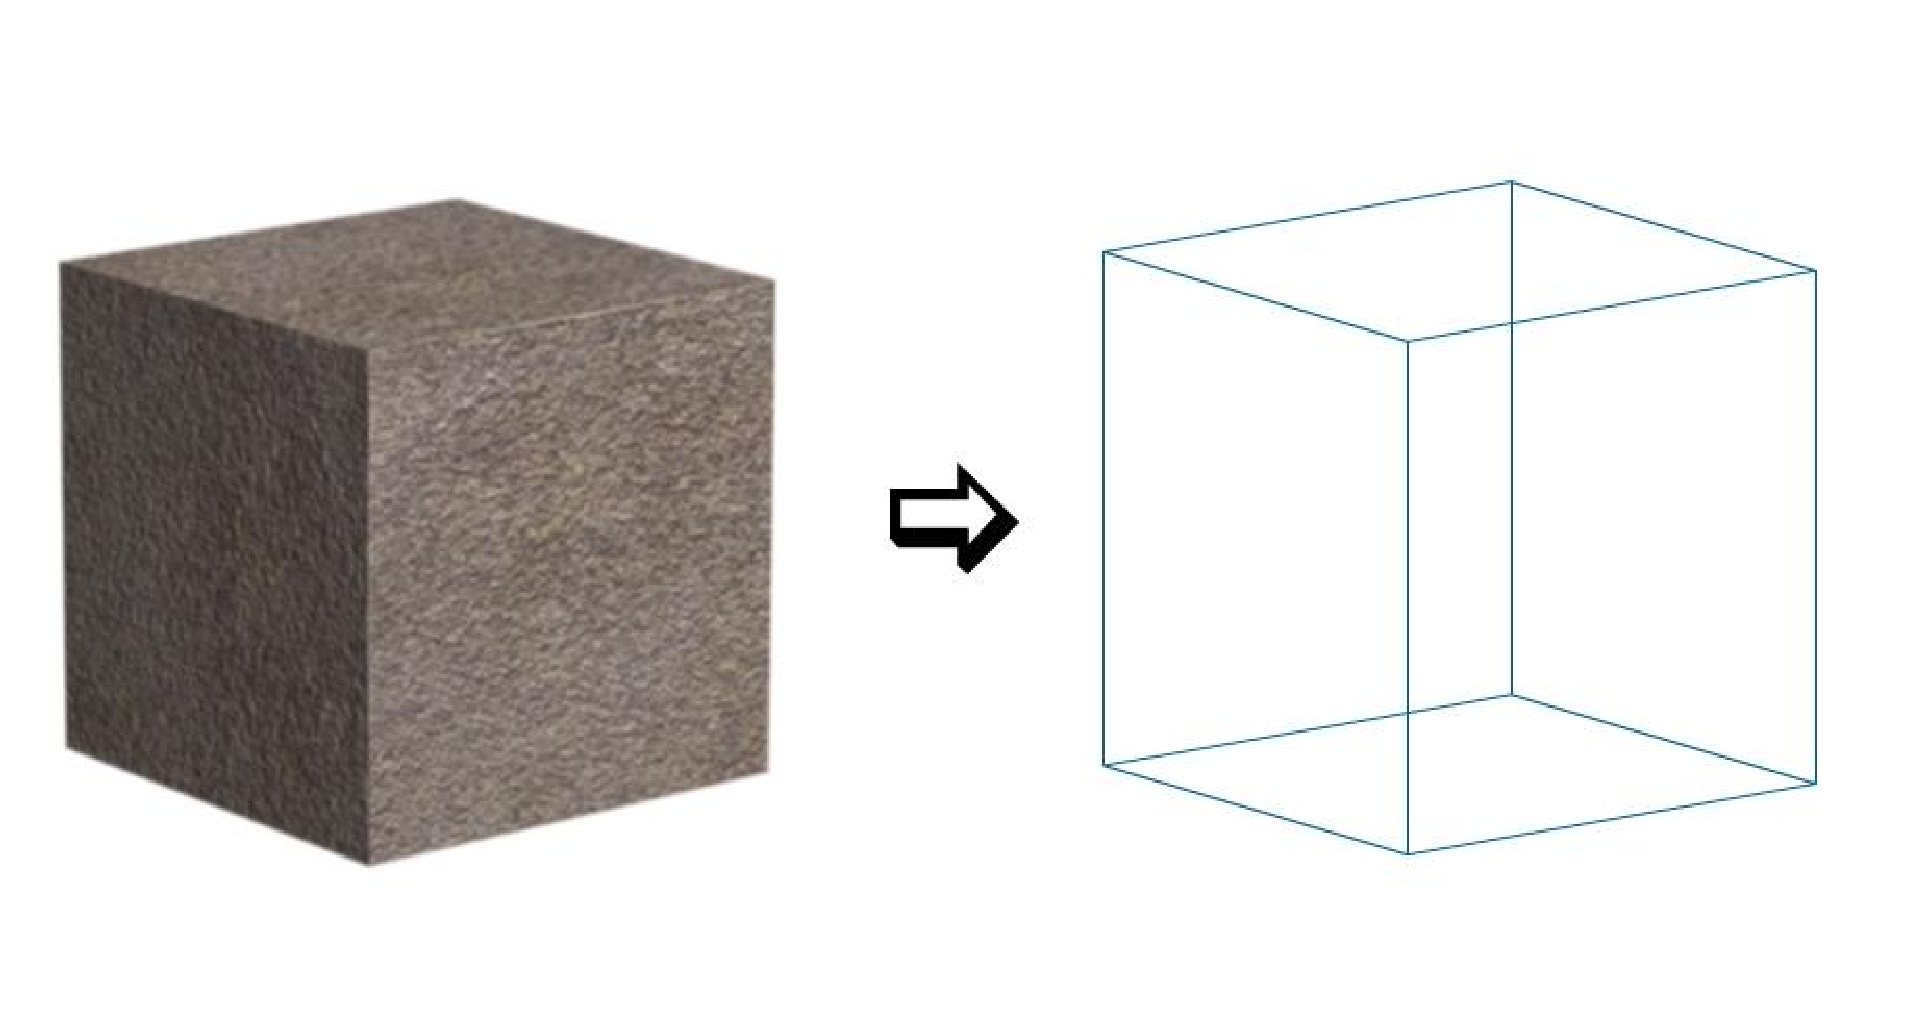
\includegraphics[scale=0.2]{wireframe}
	\caption{Representação Armada ou Wireframe.}
	\label{fg:wireframe}
\end{figure} 

\subsubsection{Representação por Faces} 
\label{sec:r_faces}
Usa faces delimitantes que descrevem os contornos do sólido. É uma das formas mais usuais na modelagem de objetos tridimensionais nos dias de hoje. Ela  também é conhecida com  \textbf{Boundary Representation} ou \textbf{B-rep}, que consiste na descrição de  objetos pelos seus contornos, ou seja, arestas e vértices. Para melhor entendimento, temos a Figura~\ref{fg:faces} como exemplo dessa representação.

\begin{figure}[ht!]
      \centering
	  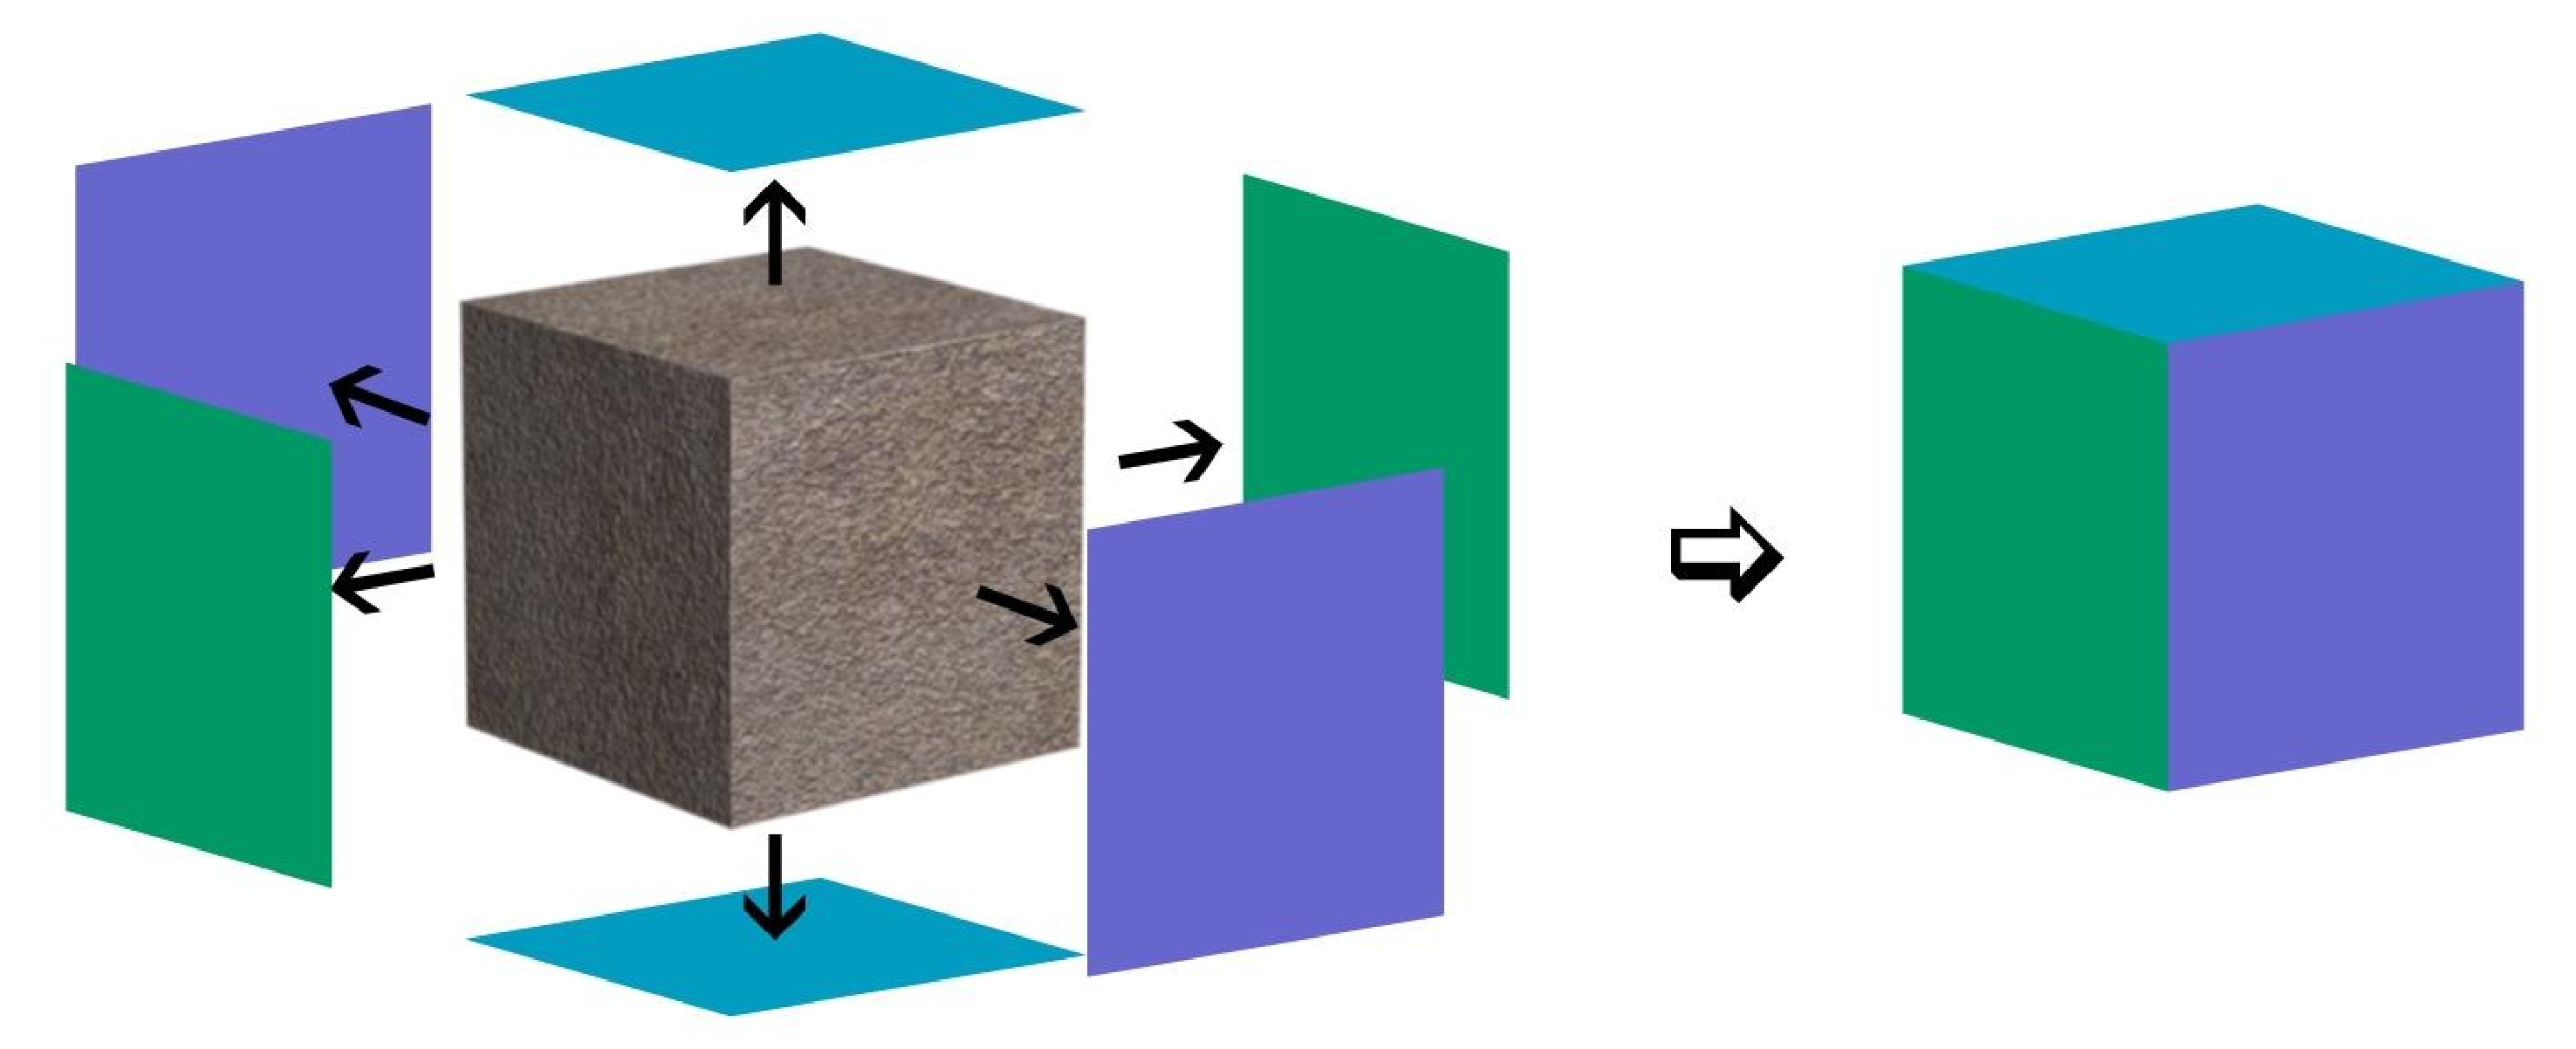
\includegraphics[scale=0.2]{faces}
	  \caption{Representação por Faces.}
	  \label{fg:faces}
\end{figure} 

\subsubsection{Representação Poligonal}
Polígono vem do grego \textit{polys}, que significa muitos , e \textit{gonos} que significa ângulos, assim esse representação é formada por figuras planas com muitos seguimentos de reta e muitos ângulos. Então podemos construir sólidos com o polígono mais  simples, o triângulo, até um mais complexo, com um número elevado de lados(Figura~\ref{fg:pilogono}). Essa técnica pode ser considerada uma especificação do caso apresentado na seção~\ref{sec:r_faces}.\\

\textit{Tesselation} é um das características dessa representação, significa preencher uma dada região através de várias repetições de um mesmo polígono até não haver mais espaços em "branco". A maioria das máquinas de jogos utilizam a representação por faces triangulares. Isso se deve ao fato de esta necessitar de menos processamento e também por possibilitar a representação de qualquer tipo de contorno\cite{traina}.

\begin{figure}[ht!]
      \centering
	  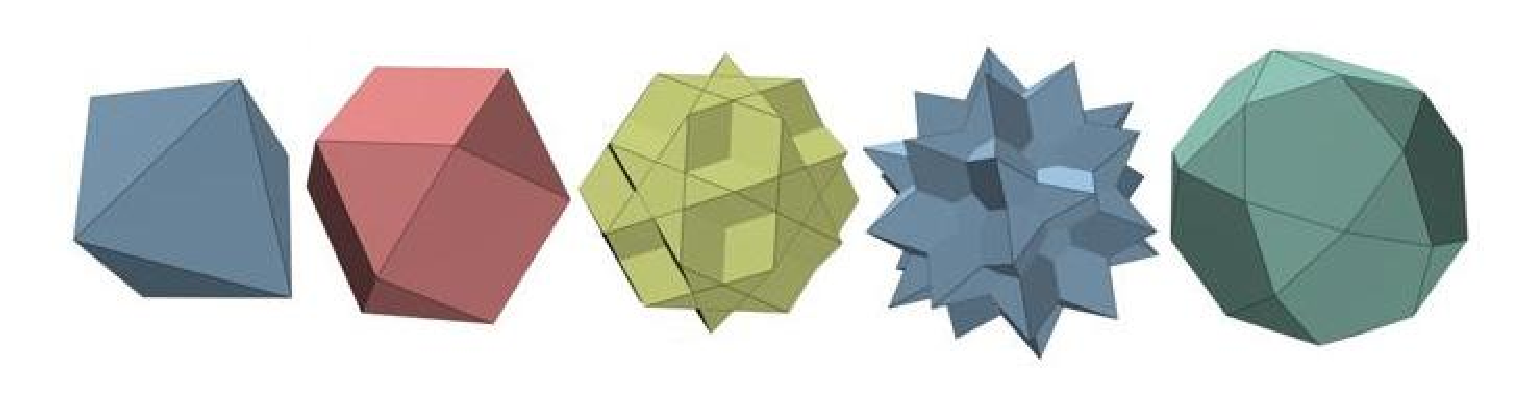
\includegraphics[scale=0.2]{poligonos}
	  \caption{Representação Poligonal.}
	  \label{fg:pilogono}
\end{figure} 

\subsection{Técnicas de Modelagem Geométrica}
Quanto ao âmbito da modelagem de objetos tridimensionais, tem-se basicamente três categorias: a manual, matemática e automática. \\

O método manual foi a base de toda a modelagem atual. É a técnica mais barata e mais antiga.  Utiliza-se basicamente das medidas do modelo real e, é claro, da habilidade do modelador. Já à matemática utiliza de algoritmos para gerar o objeto desejado. Esse método é muito utilizado para modelar, por exemplo, a proliferação de organismos microscópicos.\\

Modelagem automática é o método mais recente. Utiliza-se de scanners muitos sofisticados para obter o modelo tridimensional de qualquer ambiente ou sólido.

\subsubsection{Combinação de Objetos}
É um dos métodos mais intuitivos e antigos. É realizado através da combinação de um ou mais sólidos básico para obtenção de um outro\cite{hearn}, mostrado na Figura~\ref{fg:comb}. O  único detalhe que deve-se prestar bastante atenção nessa técnica, é a questão das operações booleanas(interseção, união e subtração) em alguns casos não gerarem como resultado um sólido, por exemplo, no caso da intercessão de dois cubos que não estão em contato, temos como resultado o vazio que não é um sólido válido.

\begin{figure}[ht!]
	\centering
	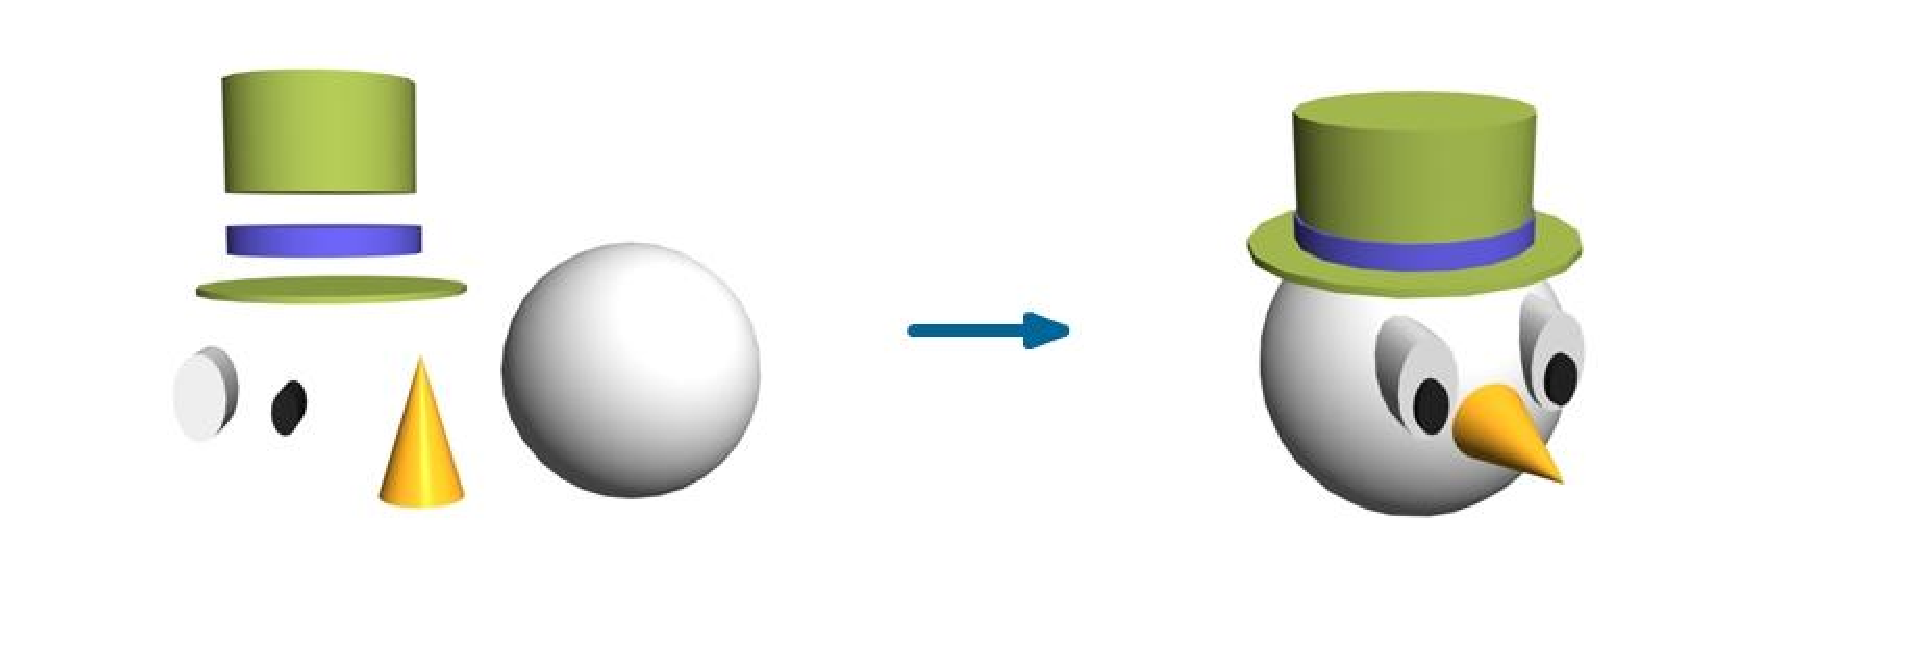
\includegraphics[scale=0.4]{montagem}
	\caption{Modelagem por Combinação de Objetos.}
	\label{fg:comb}
\end{figure} 

\subsubsection{Modelagem por Varredura(Sweep)}
A modelagem por varredura é obtida pela movimentação de uma curva $N_1$ na trajetória de uma outra curva $N_2$ que descreverá um superfície que poderá ser usada como sólido. Sendo $N_1$ nomeada de \textit{Curva de Contorno} e $N_2$ de \textit{Caminho ou Diretriz}\cite{3dsmod}.\\

Ainda no questão da varredura, pode-se sitar dois casos particulares que são: varredura por \textit{Extrusão}(Figura~\ref{fg:etrusao}) ou \textit{Translacional}(Figura~\ref{fg:rotacional}) e a \textit{Rotacional}. Para o a primeira é a translação de uma superfície na forma circular, por exemplo , ao longo de uma direção, gerando um sólido(no caso um cilindro). No segundo caso ocorre a rotação de uma superfície ao longo de um eixo ou ponto de referência, resultando também em um sólido.

\begin{figure}[ht!]
	\centering
	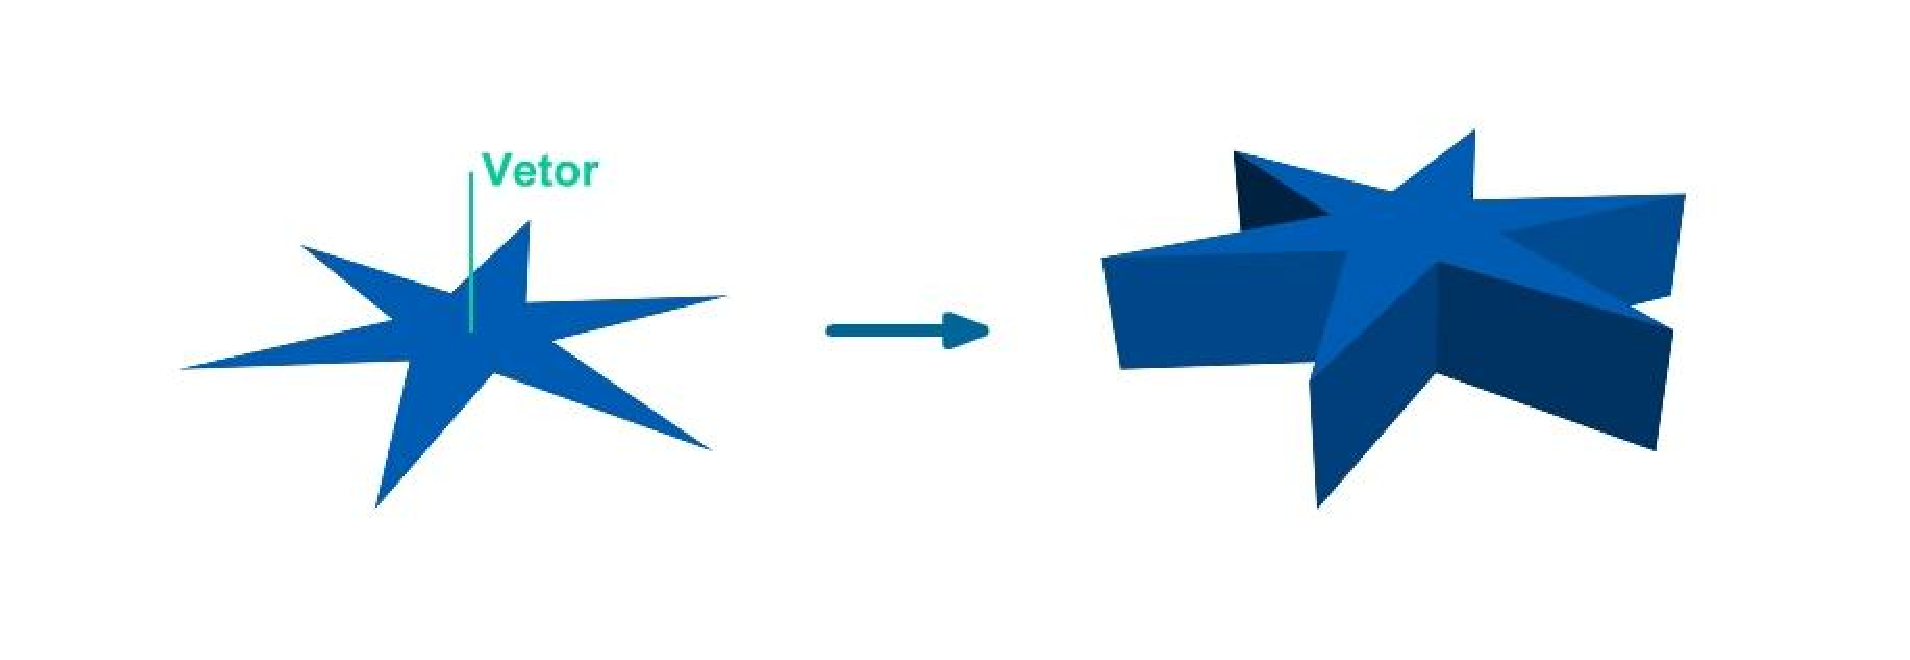
\includegraphics[scale=0.4]{extrude}
	\caption{Modelagem por Extrusão.}
	\label{fg:etrusao}
\end{figure} 
\begin{figure}[ht!]
	\centering
	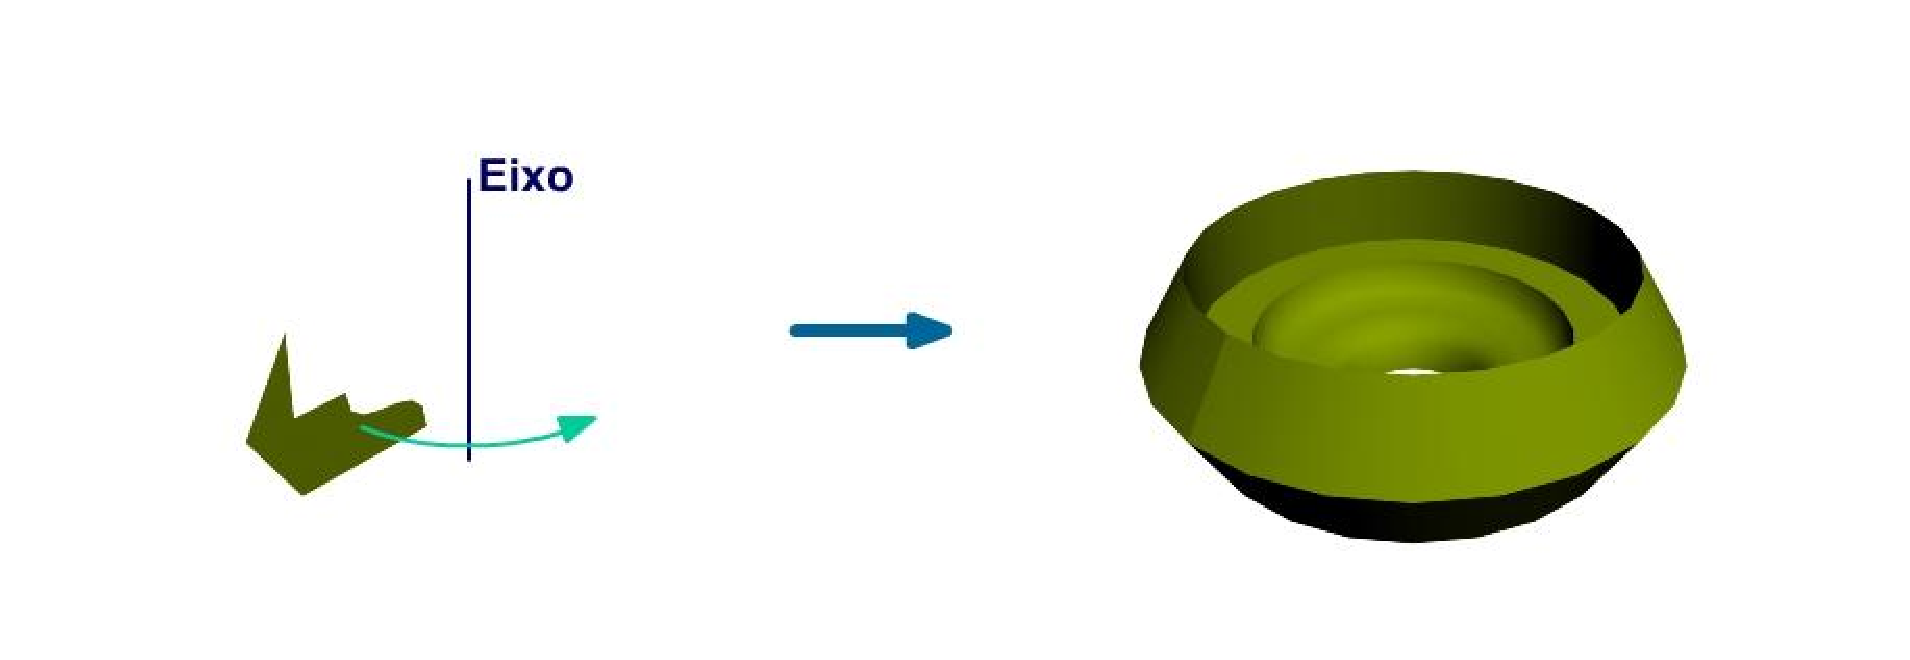
\includegraphics[scale=0.4]{rotacional}
	\caption{Modelagem Rotacional.}
	\label{fg:rotacional}
\end{figure} 

\subsection{Realidade Virtual}
O termo Realidade Virtual surgiu na década de 80 pelo artista e cientistas da computação, Jaron Lanier, que uniu os dois universos, que até então eram, muito distantes, o mundo real e o virtual\cite{jane}. Porém há registro de trabalhos anteriores a essa denominação, dentre eles esta o primeiro capacete que permitia imersão, e também pode-se falar do famoso SENSORAMA\cite{rhen}(que não obteve um grande sucesso comercial, pelo seu valor, mas com certeza foi um dos trabalhos que deram impulso para o futuro dos ambientes virtuais).\\

Mas o que é Realidade Virtual? É uma interface avançada que permite o usuário, navegar, modificar, interagir em tempo real com uma determinada aplicação. Existem basicamente dois tipos de realidade virtual quanto o fator imersão a imersiva e a não imersiva. A primeira é caraterizada por permitir ao usuário se sentir dentro do ambiente(através do uso de capacetes especiais, óculos, luvas, roupas, caves~\cite{cave}, sensores, entre outros dispositivos), já a segunda isso não ocorre(onde usa-se mouse, teclado, monitores , etc)\cite{aect}.

\subsubsection{Grafo de Cena}
É um dos conceitos mais importantes da teoria de jogos, e também da computação gráfica. Sua definição é a de ferramenta para representação de ambientes virtuais tridimensionais. Sendo esse ambiente descrito por diversos aspectos, dentre eles: descrição geométrica, câmera, transformação, aparência, comportamento e iluminação\cite{ferreira}. O cenário é formado por todos esses aspectos inseridos dentro do grafo de cena. \\

O grafo de cena é formado por nós, compondo arrestas que tem como resultado um grafo acíclico direcionado. Com cada nó tendo atributos ,sitados anteriormente, que poderão ou não influenciar nos outros nós que estão conectados a ele. Existe uma classificação para eles, que os divide em três categorias: nós raiz(é o primeiro nó, no qual todos os outros estão ligados de forma direta ou não) ,nós internos (geralmente contem informações de transformações 3D - rotação, escala e translação) e por fim estão os nós folha(que por padrão contem as dados de representação geométrica dos objetos da cena).\\ 

A propriedade fundamental dessa ferramenta é o que se chama de herança de estado. Que diz que cada nó deve herda as propriedades de estado do seus ancestrais até o nó raiz. Então se tivermos um grafo de cena formado por um \textit{nó} raiz, casa, e dois \textit{nós folha}, sendo o primeiro uma cadeira e o segundo mesa. Se rotacionarmos o \textit{nó} casa, por consequência teremos a cadeira e a mesa rotacionadas também. Porém no caso da rotação de um dos \textit{nós folha}, o \textit{nó} casa permanecerá inalterado, haja vista que ele esta hierarquicamente no nível acima e a cadeira também não se moverá pelo fato de ter uma ligação direta com esse nó(esta no mesmo nível e não tem conexão direta). Na tabela~\ref{tb:grafo_cena} estão algumas vantagens proporcionadas pelo uso dessa técnica.\\

\begin{table}
\centering
\begin{tabular}{|p{3cm}|p{8cm}|}
	\hline
	\multicolumn{2}{|c|}{Vantagens} \\ \hline
	Produtividade &  Gerencia e reduz o numero de linhas que seriam necessárias para implementar
a mesma funcionalidade utilizando uma interface de baixo nível, como a OpenGL.\\ \hline
	Portabilidade &  Encapsula todas as tarefas de baixo nível, reduzindo e até 
excluindo a parte de código que é especifica de uma plataforma.\\ \hline
	Escalabilidade &  Possibilita trabalhar tanto em máquinas com configurações básicas até supercomputadores.\\ 
	\hline
\end{tabular}
\caption{Vantagens proporcionadas pelo uso do grafo de cena.}
\label{tb:grafo_cena}
\end{table}

\section{Irrlicht}
O Irrlicht é uma máquina de jogo de alta performasse escrita em linguagem C++\cite{irrlichtbook}. Contem todas as característica que pode-se encontrar em qualquer outra \textit{engine}\footnote{Máquina de jogo.}. Existem muitos projetos desenvolvidos e em desenvolvimento usando-a, com uma boa comunidade, onde pode-se tirar dúvidas e publicar trabalhos e melhorias. E além de tudo isso, é completamente livre\cite{irrlicht}.\\

Ela tem como principais características:
\begin{enumerate}
\item Renderização em tempo real de alta performasse usando \textbf{Direct3D} e \textbf{OpenGL}.
\item Independe de plataforma.
\item Renderiza diretamente de arquivos, tais como : .zip, .pak, .pk3, etc.
\item Rápida e fácil detecção de colisão.
\item Possibilita o uso de vários linguagens de programação, como : Java, Delphi, entre outras.
\item Limpa, fácil de entender, e bem documentada.
\end{enumerate}

\section{Método FDTD}
O termo Método FDTD(Finite-Differene Time-Domain Method), primeiramente chamado de como Algorítimo de Yee, foi criado por Kane Yee em 1966\cite{yeebook}. É uma técnica capaz de solucionar, de forma simples e elegante, numericamente as equações de Maxwell, de maneira direta. Tem como características principais: 1)distribuição geométrica discreta das componentes de campos Elétrico e Magnético em células, de maneira a satisfazer tanto a Lei de Faraday quanto a Lei de Ampère nas formas diferencial e integral e 2)aproximação das derivadas espaciais e temporais por diferenças finitas, de forma a se obterem equações explicitas para a atualização temporal de todas as componentes de campo\cite{rodrigo}.\\

Porém, por algum tempo, esse método foi deixado de lado devido ao fato de ter um custo computacional muito alto, aliado a isso, deve-se levar em consideração o contexto histórico em que ele se encontrava, onde os computadores ainda eram bem limitados. Mas, um tempo depois, ressurgiu através dos trabalhos de dois cientistas, chamados Allen e Brodwin, que aplicaram essa técnica para problemas tridimensionais relacionados à interação eletromagnética com meios materiais\cite{allen}. Assim, novas técnicas apareceram e melhoram a abordagem do método, acompanhado , é claro, da evolução dos computadores.\\

Essa técnica tem sido usada desde então, em uma grande quantidade de aplicações, entre elas estão: radares, antenas, fotônica, sistemas de telecomunicação, medicina, estruturas periódicas, sistemas de aterramento, entre várias outras.\\

O método FDTD aplicado com intuito de simular uma propagação eletromagnética, utiliza as equações de Maxwell na forma diferencial.
\begin{equation}\label{eq:faraday}
	\overline{\nabla}\times\overline{E}=-\mu\frac{\partial \overline{H}}{\partial t},
\end{equation}
\begin{equation}\label{eq:ampere}
		\overline{\nabla}\times\overline{H}=\epsilon\frac{\partial \overline{E}}{\partial t} + \overline{J},
\end{equation}
		
	Onde:\\
	$\overline{J} = \sigma\overline{E}$, vetor densidade de corrente elétrica  de condução(ampere/$m^{2}$).\\ 

As equações (\ref{eq:faraday}) e (\ref{eq:ampere}) expandidas em coordenadas retangulares, geram as respectivas equações escalares, mostradas abaixo.
\begin{equation}
	\frac{\partial H_x}{\partial t} = \frac{1}{\mu}(\frac{\partial E_y}{\partial z}-\frac{\partial E_z}{\partial y}),
\end{equation}
\begin{equation}
	\frac{\partial H_y}{\partial t} = \frac{1}{\mu}(\frac{\partial E_z}{\partial x}-\frac{\partial E_x}{\partial z}),
\end{equation}
\begin{equation}
	\frac{\partial H_z}{\partial t} = \frac{1}{\mu}(\frac{\partial E_x}{\partial y}-\frac{\partial E_y}{\partial x}),
\end{equation}

\begin{equation}
	\frac{\partial E_x}{\partial t} = \frac{1}{\epsilon}(\frac{\partial H_z}{\partial y}-\frac{\partial H_y}{\partial z} -\sigma E_x),
\end{equation}
\begin{equation}
	\frac{\partial E_y}{\partial t} = \frac{1}{\epsilon}(\frac{\partial H_x}{\partial z}-\frac{\partial H_z}{\partial x} -\sigma E_y),
\end{equation}
\begin{equation}
	\frac{\partial E_z}{\partial t} = \frac{1}{\epsilon}(\frac{\partial H_y}{\partial x}-\frac{\partial H_x}{\partial y} -\sigma E_z)
\end{equation}

sendo:\\
$E_x, E_y, E_z$ e $H_x, H_y, H_z$ representam as componentes dos campos elétrico $\overline{E}$ e magnético $\overline{H}$, respectivamente. Essas componentes são funções do tempo $t$ e das três coordenadas cartesianas ($x,y,z$).\\

A lei de Faraday, equação (\ref{eq:faraday}), informa que quando há variação no tempo do vetor $\overline{B}=\mu\overline{H}$ (vetor densidade de fluxo magnético, em teslas), surgem componentes de campo elétrico circulando em torno da(s) componente(s) deste vetor. Já a lei de Ampère, equação (\ref{eq:ampere}), informa que quando há variação no tempo do vetor $\overline{D}=\epsilon\overline{E}$ (vetor densidade de fluxo elétrico, em ) em certa direção e/ou a presença da fonte de corrente $\overline{J}$, esta causa circulação de campo magnético em torno da direção da(s) componente(s) deste vetor.\\
			
Kane Yee se baseou nessa duas observações para definir seu esquema  de distribuição espacial  e temporal das componentes  de campo  de seu algoritmo. Sua representação geométrica, chamada de célula de Yee, esta mostrada na Figura \ref{fg:celulaYee}\cite{rodrigo}.\\
			
\begin{figure}[ht!]
\centering
	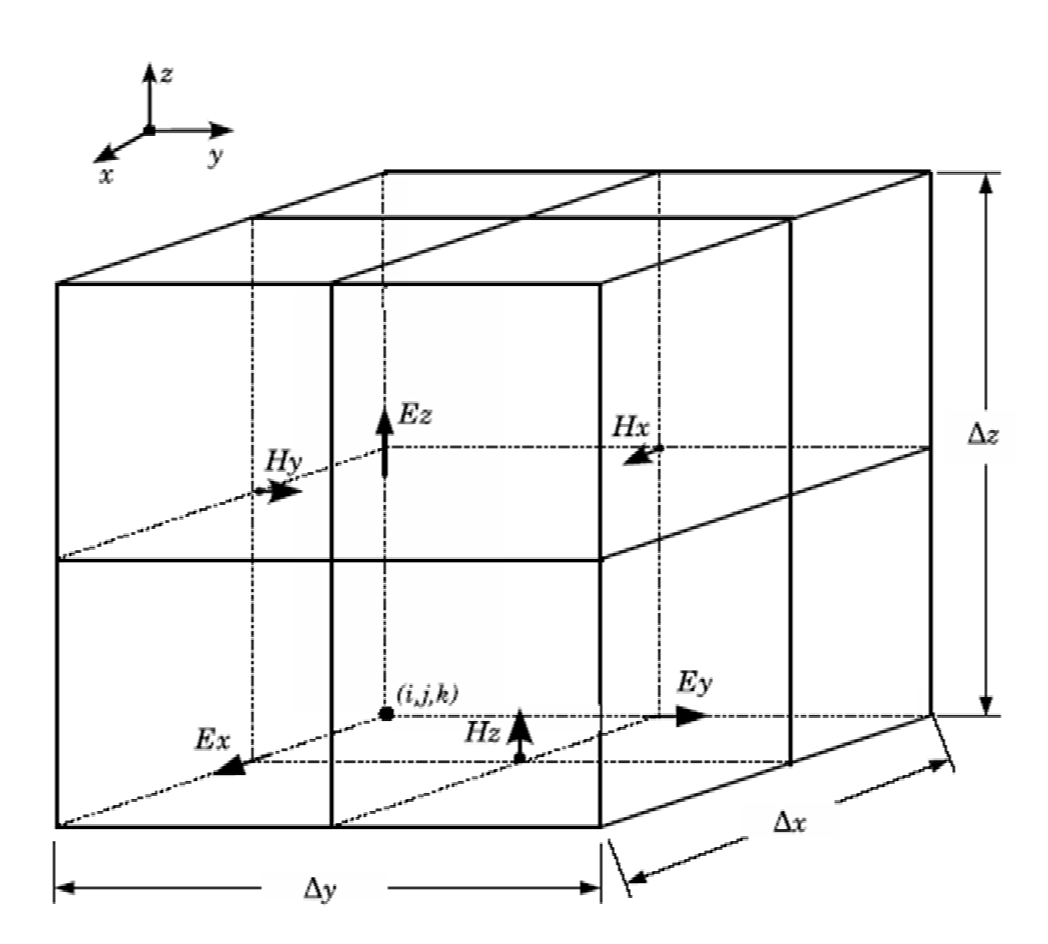
\includegraphics[scale=0.5]{celula}
	\caption{Célula Yee.}
	\label{fg:celulaYee}
\end{figure} 
		
Para que possam ser realizadas simulações de propagação de onda em FDTD, é criada uma malha 3D formada por múltiplas células de Yee que preenche toda região de análise, Figura\ref{fg:grade}\cite{almeida}, com a finalidade de mostrar as componentes de campo $\overline{E}$ e $\overline{H}$ atuantes em cada ponto da malha desta região.	\\
\begin{figure}[ht!]
	\centering
	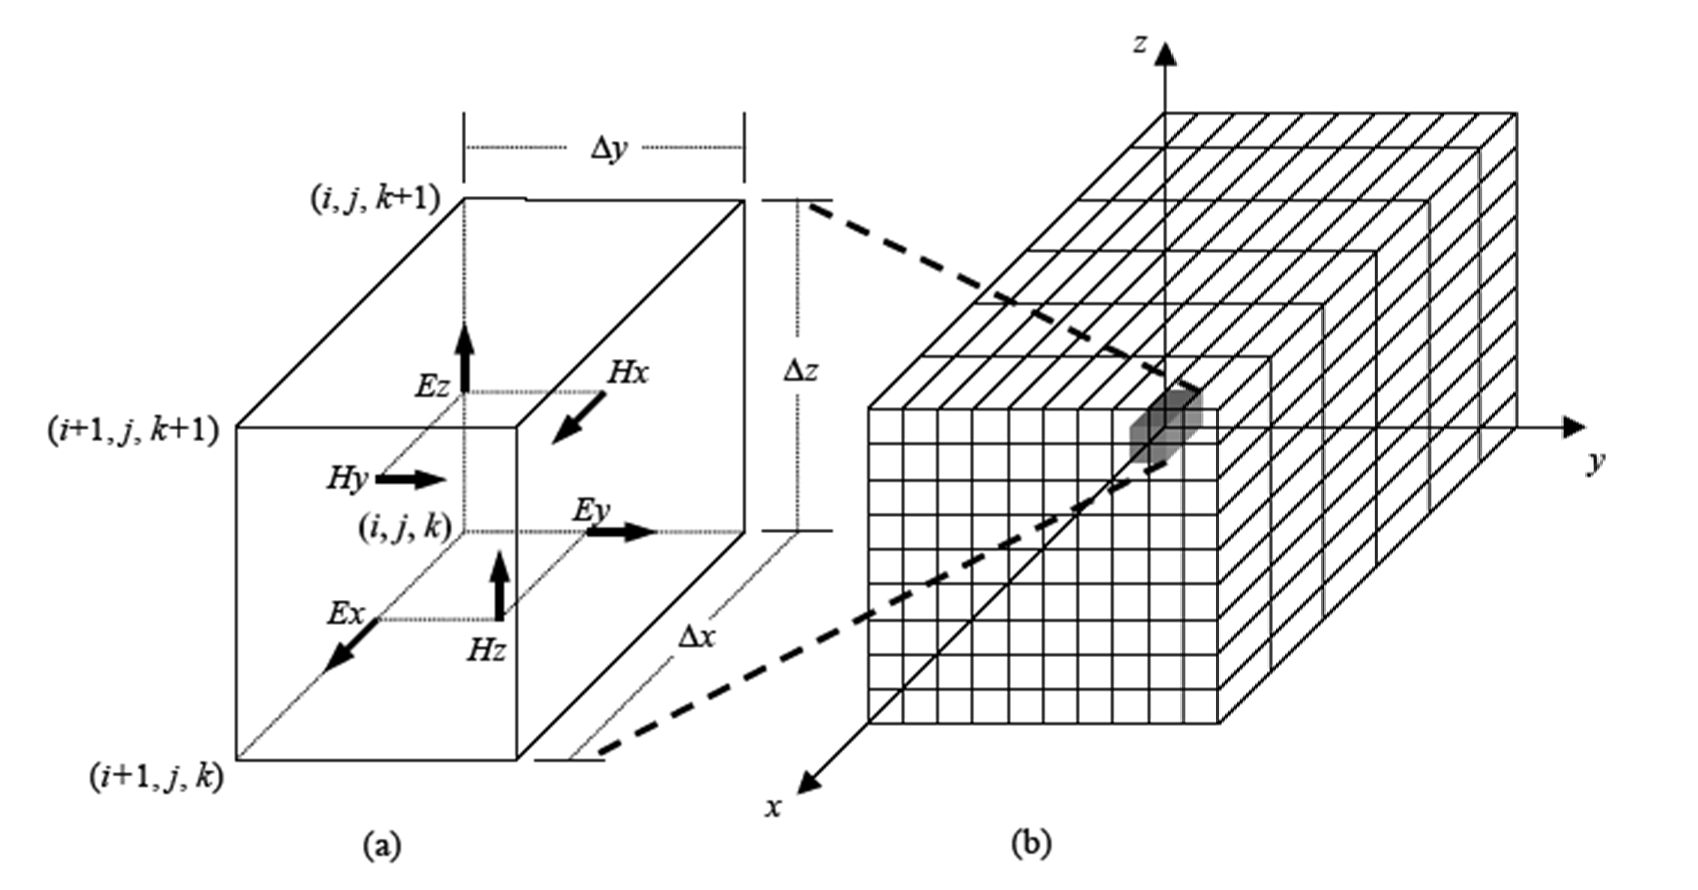
\includegraphics[scale=0.5]{Malha3D}
	\caption{(a) Posição das componentes dos campos elétrico e magnético em uma célula de Yee;(b) Célula no interior de uma malha 3-D.}
	\label{fg:grade}
	\end{figure} 

A referência a cada célula que compõe a malha, assim com as suas respectivas componentes de campo, é feita de forma discreta pelos índices $i, j$ e $k$, de forma que uma determinada posição $x, y, z$ (em metros) é referenciada no espaço discreto por $i, j, k$ (número da célula correspondente). Estas  referências são obtidas através das relações $x = i.\Delta_x, y = j.\Delta_{y}$ e $z = k.\Delta_z$, onde  $\Delta_x,  \Delta_y$ e $\Delta_z$ são as dimensões das células de Yee(Figura\ref{fg:celulaYee}).


\chapter{Desenvolvimento do Software}
	O \textit{software} de computadores é a tecnologia mais importante no palco mundial, pelo fato de ter assumido um duplo papel; é o produto e, ao mesmo tempo o veículo para entrega do produto. Como produto, é um transformador de informações - produzindo, gerindo, modificando e exibindo informações que podem ser tão simples como um \textit{bit} ou tão complexas quando uma vídeo aula. Como veículo, o \textit{software} age como base para controlar o computador (sistemas operacionais),  para a comunicação da informação (redes de computadores) e para criação e controle de outros programas (ferramentas e ambientes de desenvolvimento)~\cite{engsoftware}.

	Com toda esse importância,  a área de desenvolvimento de \textit{softwares} cresceu de forma avassaladora, exigindo assim uma padronização, haja vista que todo sistema (\textit{software}) necessita de reparos e melhorias à medida que o tempo passa. Por estes motivos surge a engenharia de \textit{software}, que é um conjunto de métodos e ferramentas que auxiliam no projeto, desenvolvimento, testes e manutenção de um \textit{software}.

\section{Modelo de Processo de Software}
	O modelo de desenvolvimento de software utilizado neste projeto foi o incremental. Ele consiste em um processo iterativo, que objetiva entregar o produto operacional a cada incremento~\cite{engsoftware}.

	Os primeiros incrementos são versões simplificadas do produto final, que oferecem capacidades mínimas de utilização por parte do usuário. A figura~\ref{fg:engsoftware} ilustra como este modelo se comporta durante o tempo estimado para o projeto.
\begin{figure}[ht!]
	\centering
	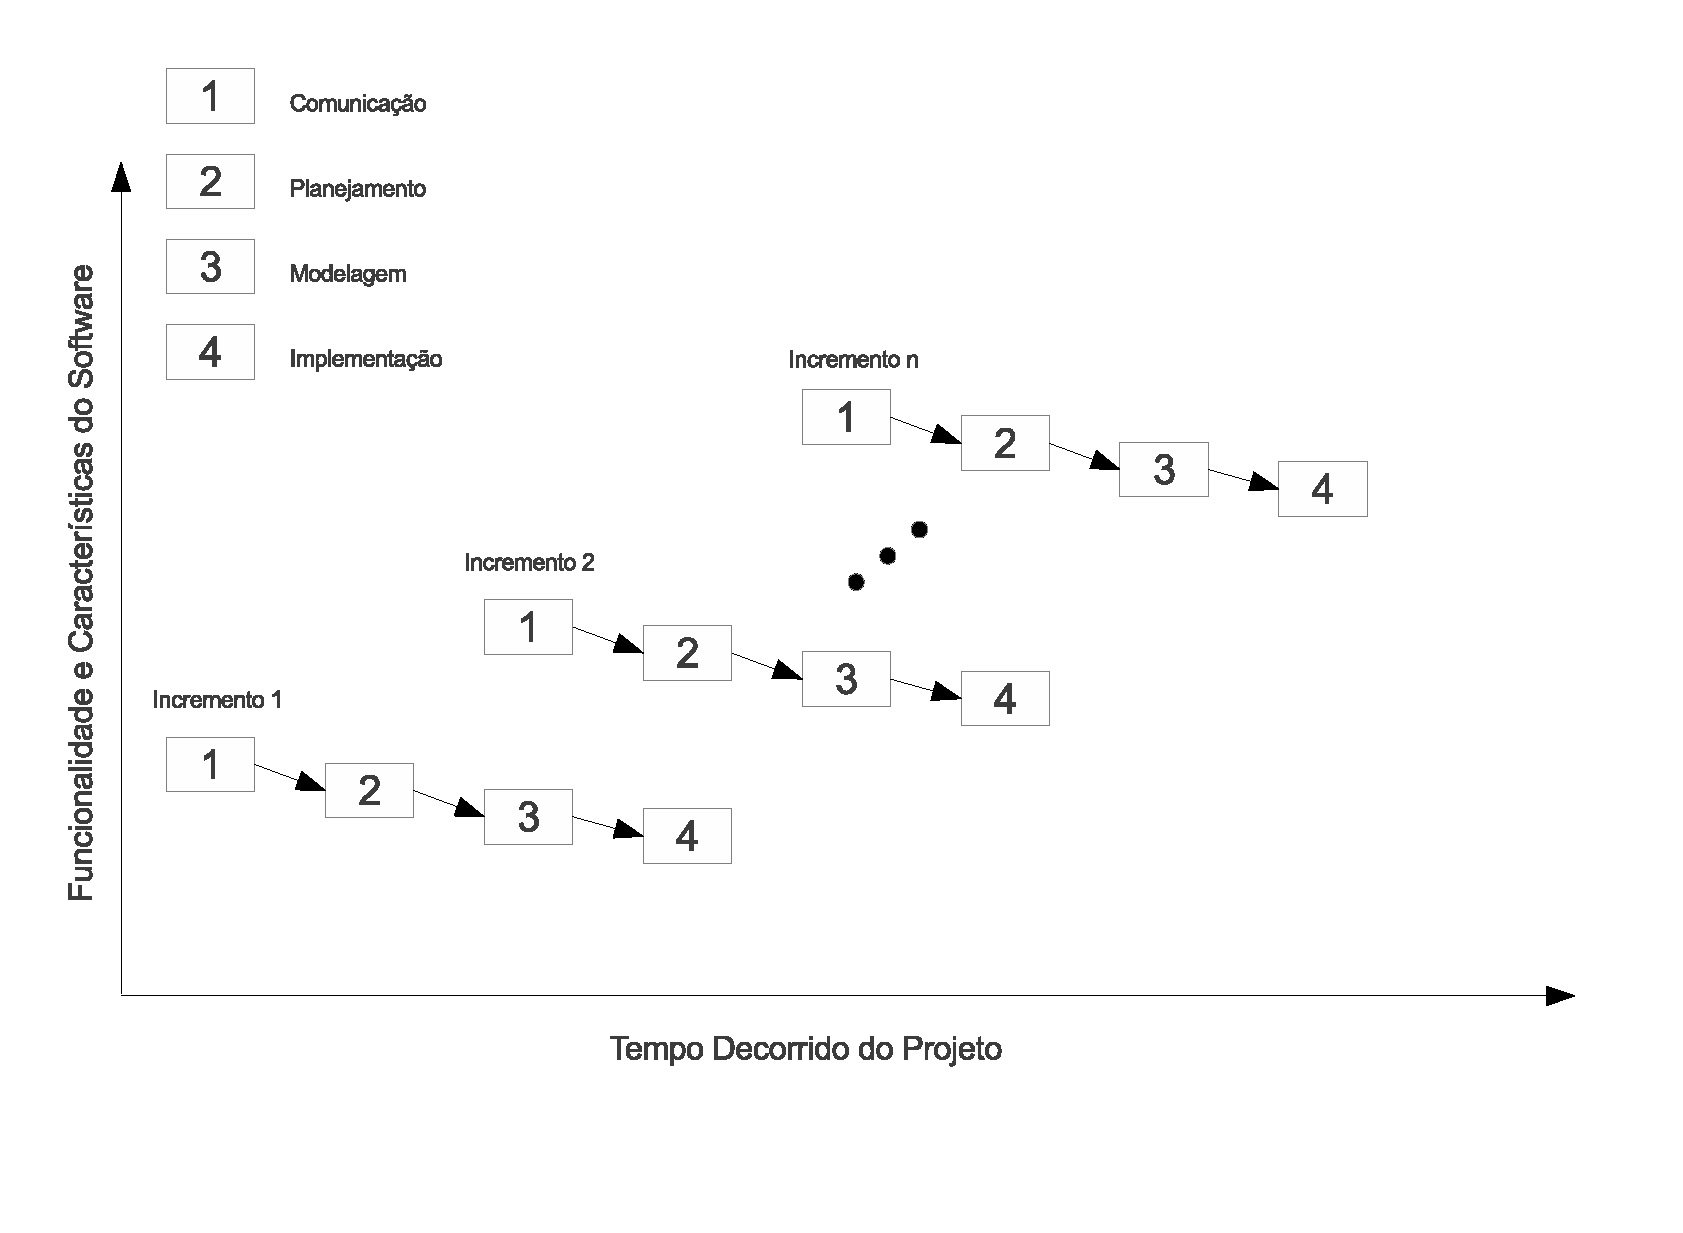
\includegraphics[scale=0.5]{engsoftware}
	\caption{Diagrama do modelo de desenvolvimento incremental.}
	\label{fg:engsoftware}
\end{figure} 

	Estão descritas abaixo, as etapas deste modelo:
\begin{enumerate}
	\item \textbf{Comunicação:} é responsável pelo levantamento do(s) propósito(s) do projeto.
	\item \textbf{Planejamento:} tem o papel de definir os requisitos do trabalho.
	\item \textbf{Modelagem:} define as ferramentas, linguagens, etapas a serem desenvolvidas.
	\item \textbf{Construção:} é o processo de codificação e testes.
	\item \textbf{Implementação:} responsável pela entrega do protótipo (inicial ou final).
\end{enumerate}

\section{Tecnologias de Programação Usadas}
	As tecnologias de programação usadas neste projeto foram: o motor de jogos \textit{Irrlicht}, a plataforma \textit{Qt-Creator} e a linguagem C++. 

	O \textit{Irrlicht} é uma máquina de jogo de alta performance escrita em linguagem C++\cite{irrlichtbook}.  Tem no fato de ser \textit{open source}~(código aberto), uma das suas principais vantagens em relação a outras \textit{engines}~(proprietárias). Abaixo estão listadas, outras características deste motor gráfico~\cite{irrlicht}. 
\begin{enumerate}
\item Renderização em tempo real de alta performance usando \textbf{Direct3D} e \textbf{OpenGL}.
\item Independe de plataforma.
\item Renderiza diretamente de arquivos, tais como : .zip, .pak, .pk3, etc.
\item Rápida e fácil detecção de colisão.
\item Possibilita o uso de vários linguagens de programação, como : C/C++, Java, Delphi, entre outras.
\item É limpa, fácil de entender, e bem documentada.
\end{enumerate}

	 O \textit{Qt-Creator} é um poderoso ambiente multi plataforma que permite a criação de diversas aplicações \textit{web} e também \textit{desktop}. Sua importância, neste trabalho, está relacionada com oferecer suporte para a criação de uma interface \textit{desktop}, a qual pudesse ser usada em diferentes sistemas operacionais~(Linux, Windows ou Macintoch) e com arquiteturas dissemelhantes~(32 ou 64 bits), para modelar tanto objetos 3D básicos como ambientes \textit{indoor}. 

	O C++ é uma linguagem orientada a objeto utilizada por milhares de programadores em inúmeros domínios de aplicação. Ela é sustentada por um conjunto vasto de bibliotecas, livros, revistas técnicas e conferências. É tão robusta que está presente no desenvolvimento (total ou de partes) de muitos sistemas operacionais. 

	Tanto as plataformas (\textit{Irrlicht} e \textit{Qt}) quanto a linguagem de programação C/C++, foram escolhidas por serem muito usadas pelo comunidade desenvolvedora por mostrarem robustez,  boa documentação e  terem uma conexão~(tanto o \textit{Irrlicht} quanto o \textit{Qt} usam a linguagem C++).

\section{Classes}
	O uso do conceito de classes, na implementação deste trabalho, se dá ao fato de que a linguagem C++ baseia-se no paradigma da orientação a objeto. A orientação a objeto é um conjunto de conceitos no qual o desenvolvimento (analise, projeto e programação) de sistemas de software está baseada na composição e iteração entre diversas unidades de software chamadas de objetos. Alguns de seus conceitos essenciais são:

\begin{itemize}
	\item \textbf{Classe}: representa um conjunto de objetos com características afins. Uma classe define o comportamento dos objetos através de seus métodos, e quais estados ele é capaz de manter através de seus atributos.
	\item \textbf{Objeto}: um objeto é capaz de armazenar estados através de seus atributos e reagir a mensagens enviadas a ele, assim como se relacionar e enviar mensagens a outros objetos.
	\item \textbf{Atributos}: são elementos que definem a estrutura de uma classe.
	\item \textbf{Métodos}: especificam a forma como os dados de um objeto são manipulados.
	\item \textbf{Herança}: é um princípio que permite que classes compartilhem atributos e métodos.
\end{itemize}

	As classes criadas para este projeto foram: \textit{IrrViewer, Cena, IrrNode, ReceiverEvent} e \textit{MainWindow}. O diagrama \textit{uml} mostrado na Figura ~\ref{fg:classes}, está representando o relacionamento entres estas classes.

\begin{figure}[ht!]
	\centering
	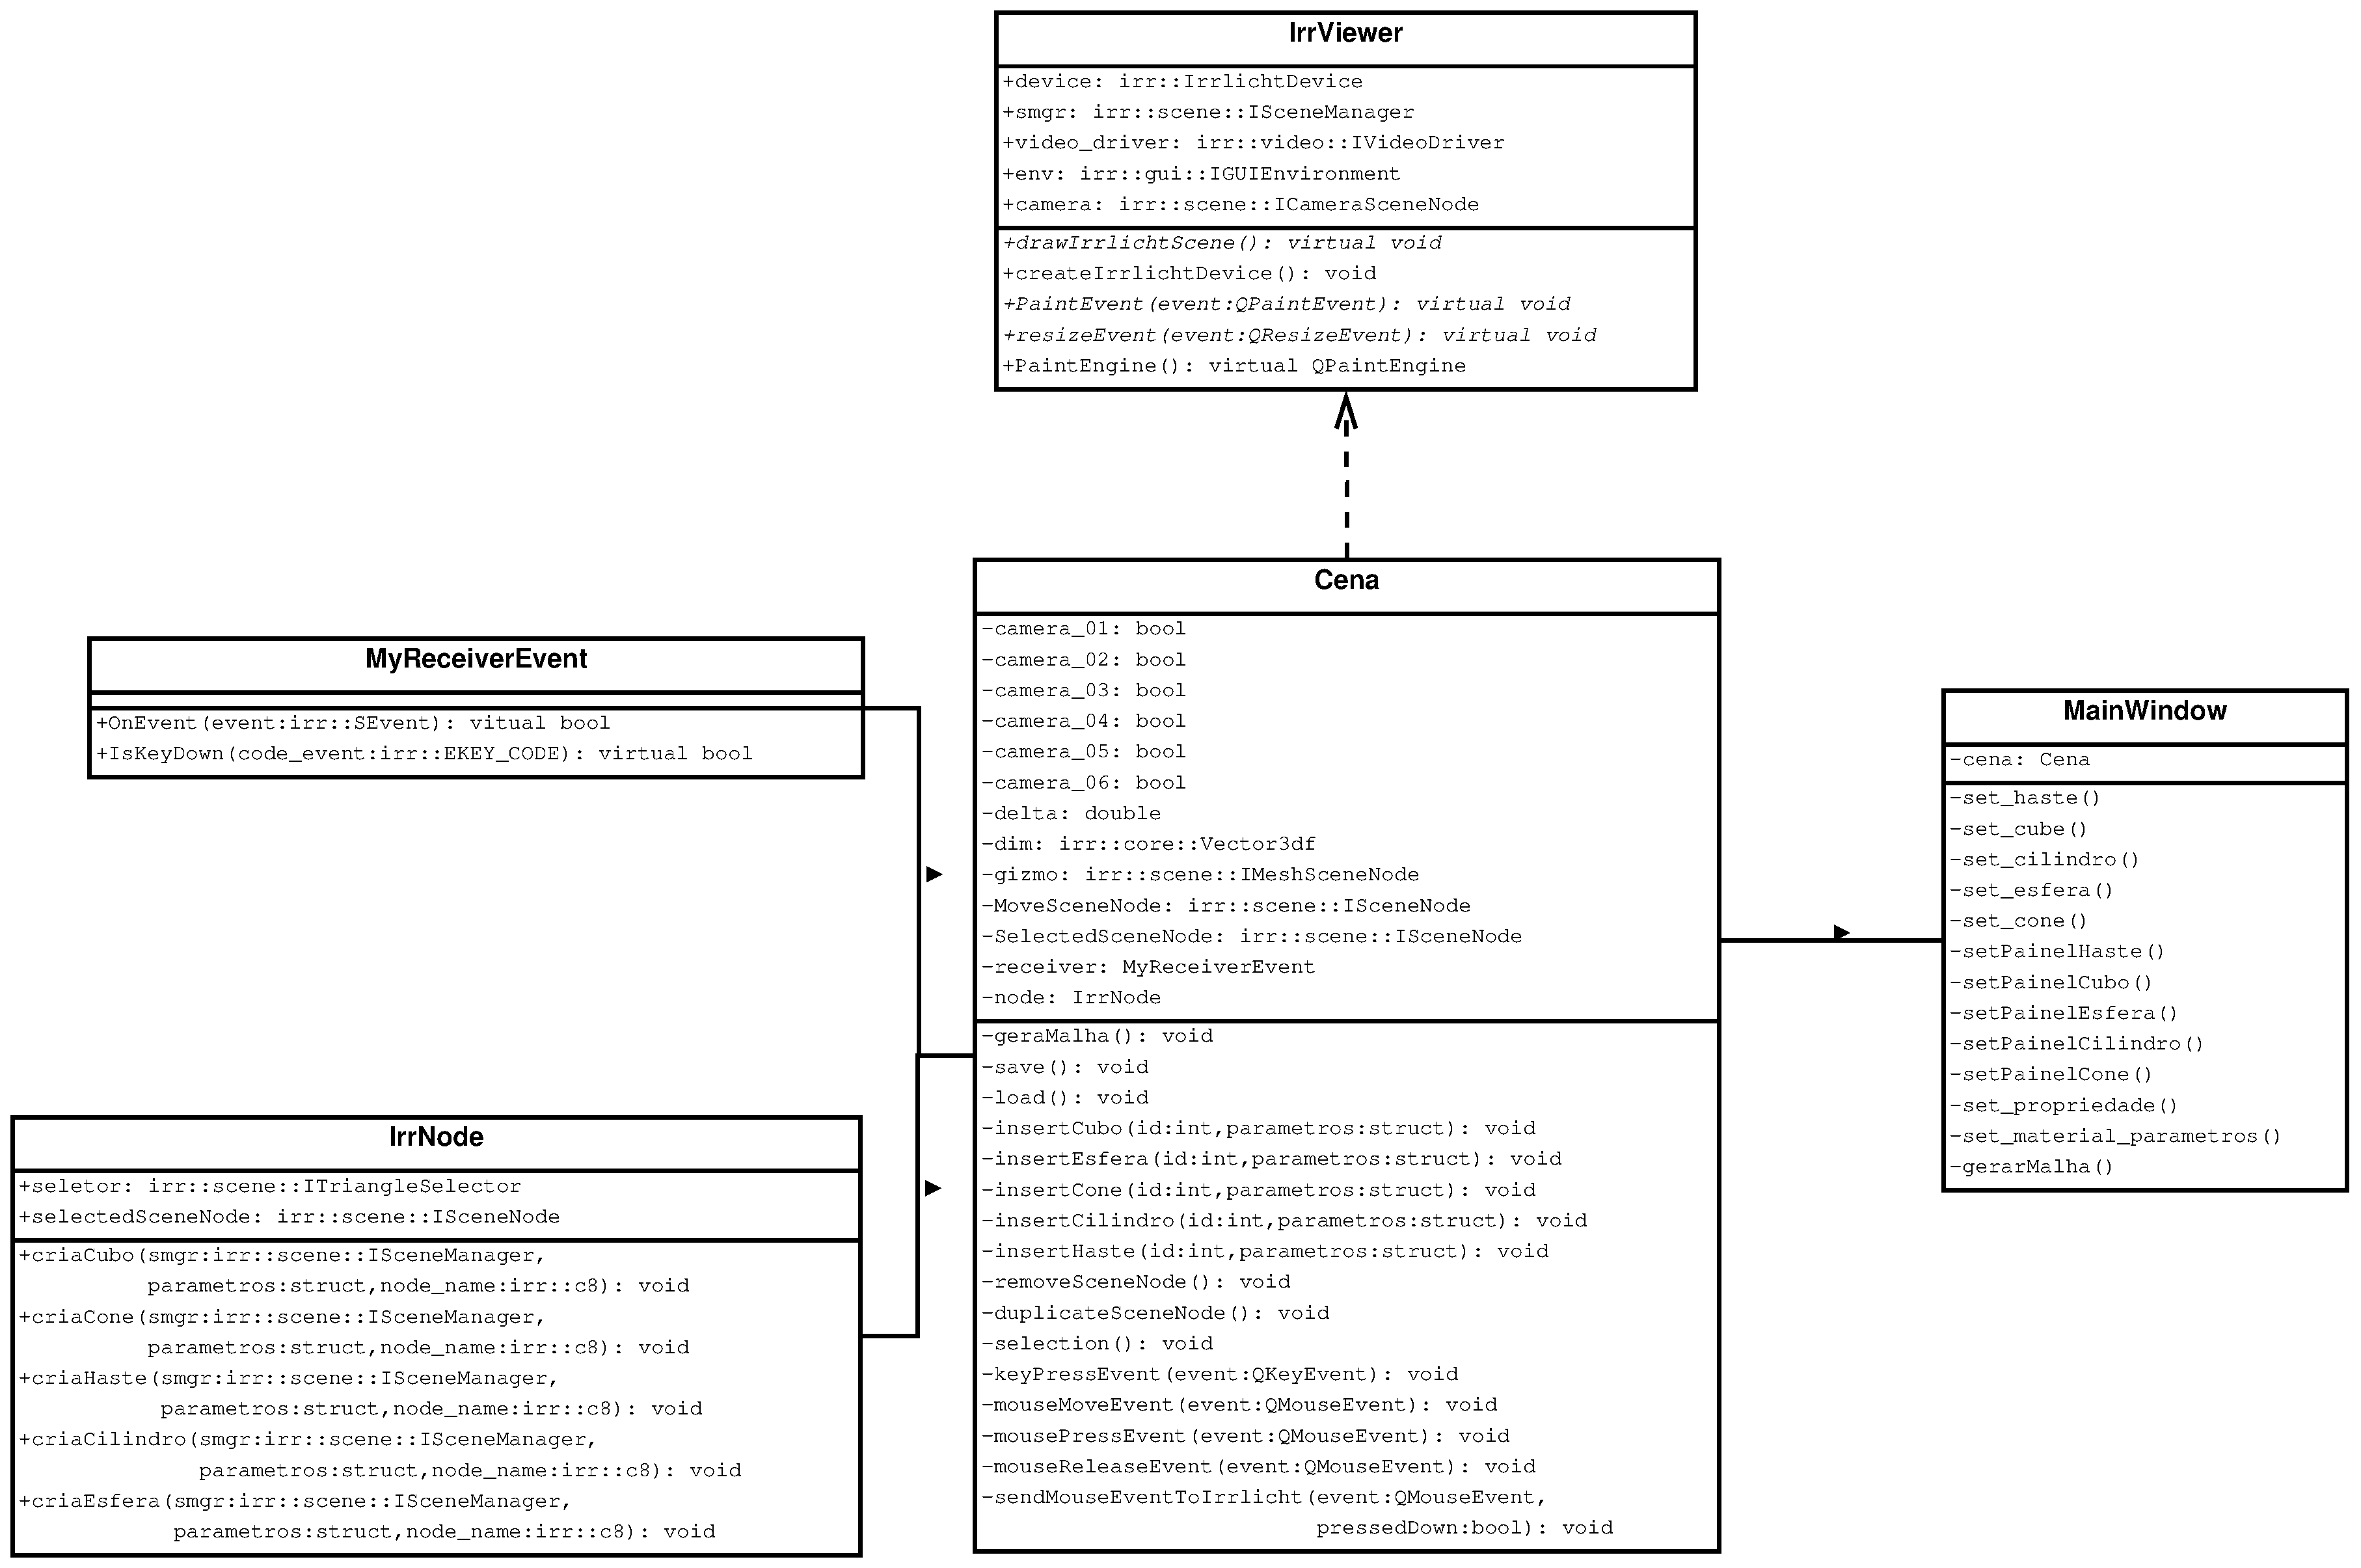
\includegraphics[scale=0.25]{classes}
	\caption{Diagrama \textit{uml} do relacionamento das classes desenvolvidas neste projeto.}
	\label{fg:classes}
\end{figure} 

	O primeiro passo no desenvolvimento deste trabalho foi a união do motor de jogos \textit{Irrlicht} com a plataforma \textit{Qt-Creator}, necessitava-se que a cena \textit{Irrlicht} fosse reconhecida como uma janela padrão do \textit{Qt} (para poder introduzi-la na interface ). Para tanto, foi necessário o estudo das classes básicas destes dois universos, assim como suas principais características. 

	Esta união foi concretizada por meio da criação da classe \textit{IrrViewer}, que contêm tantos os métodos que caracterizam uma classe \textit{Widget} quanto os necessários para criação de um cenário \textit{Irrlicht}. A Figura~\ref{fg:classeirrviewer} ilustra os principais atributos e métodos desta classe.
\begin{figure}[!ht]
	\centering
	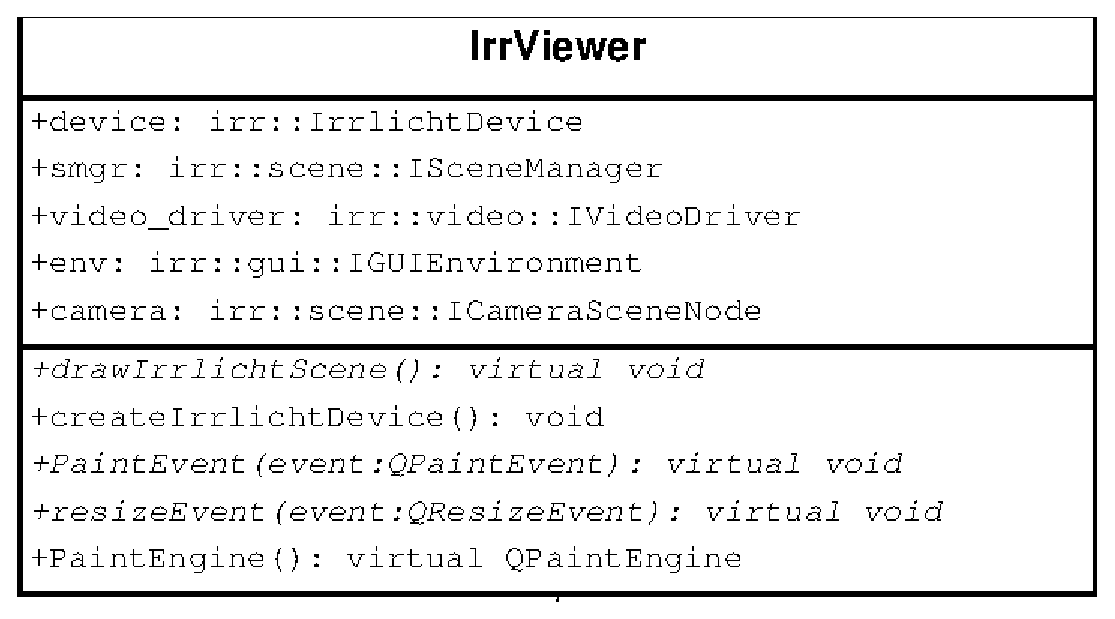
\includegraphics[scale = 0.4]{classeirrviewer}
	\caption{Classe IrrViewer.}
	\label{fg:classeirrviewer}
\end{figure}

	Assim, com o \textit{Qt-Creator} reconhecendo essa nova classe como uma de suas janelas(Widget), pode-se passar para segunda fase do projeto (desenvolvimento de outras classes e métodos necessários para preenchimento dos requisitos pré-estabelecidos).

	A classe MyReceiverEvent(Fig.~\ref{fg:classereceiverevent}) foi criada com intuito de comunicar o  evento de \textit{mouse} do \textit{Qt} com a \textit{engine Irrlicht}. Desta forma, quando este evento for disparado ( chamado ), passará para o objeto desta classe o estado do \textit{mouse} que será tratado e enviado para o \textit{Irrlicht}. 
\begin{figure}[!ht]
	\centering
	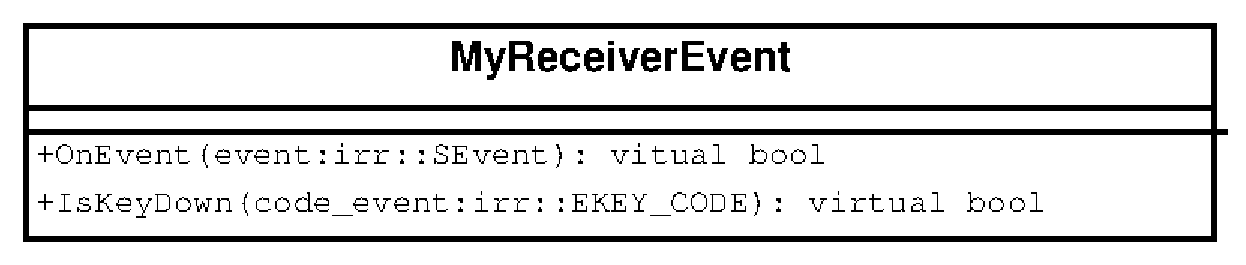
\includegraphics[scale = 0.4]{classereceiverevent}
	\caption{Classe ReceiverEvent.}
	\label{fg:classereceiverevent}
\end{figure}

	O papel de dar suporte à criação de objetos tridimensionais para o cenário virtual foi designado a classe \textit{IrrNode} (Fig.~\ref{fg:classeirrnode}). Portanto esta contém a implementação dos métodos de construção dos todos os objetos 3D básicos suportados pela interface criada neste trabalho, tais como os de criação de cubos, esferas, hastes, cilindros e cones.
\begin{figure}[!ht]
	\centering
	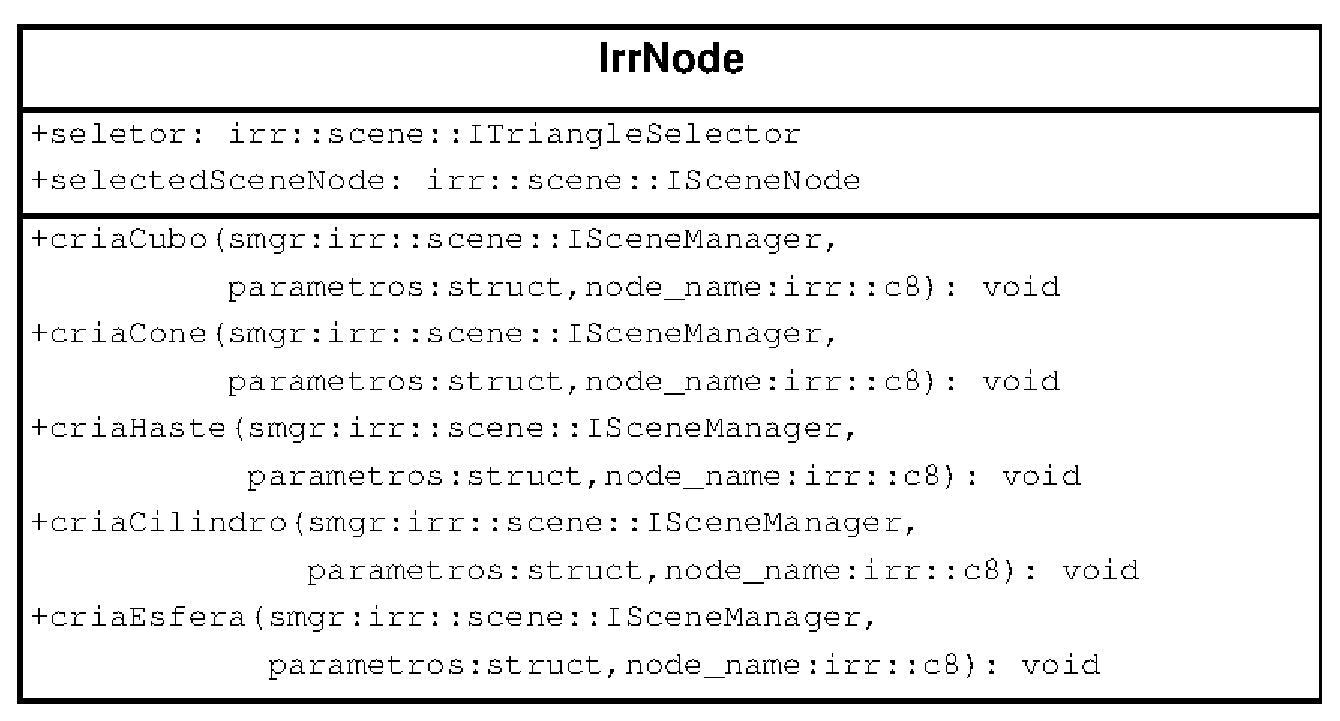
\includegraphics[scale = 0.4]{classeirrnode}
	\caption{Classe IrrNode.}
	\label{fg:classeirrnode}
\end{figure}

	Já os atributos e métodos necessários para modificação do cenário virtual estão presentes na classe \textit{Cena}~(\ref{fg:classecena}). Sendo ela, desta forma, a responsável pelo gerenciamento de todo e qualquer evento que ocorra dentro do AV. Ela faz isso, utilizando-se dos : objetos das classes \textit{IrrNode} e \textit{MyReceiverEvent}, dos métodos herdados da classe \textit{IrrViewer} (olhar Figura~\ref{fg:classes}) e dos seus próprios métodos e atributos. 
\begin{figure}[!ht]
	\centering
	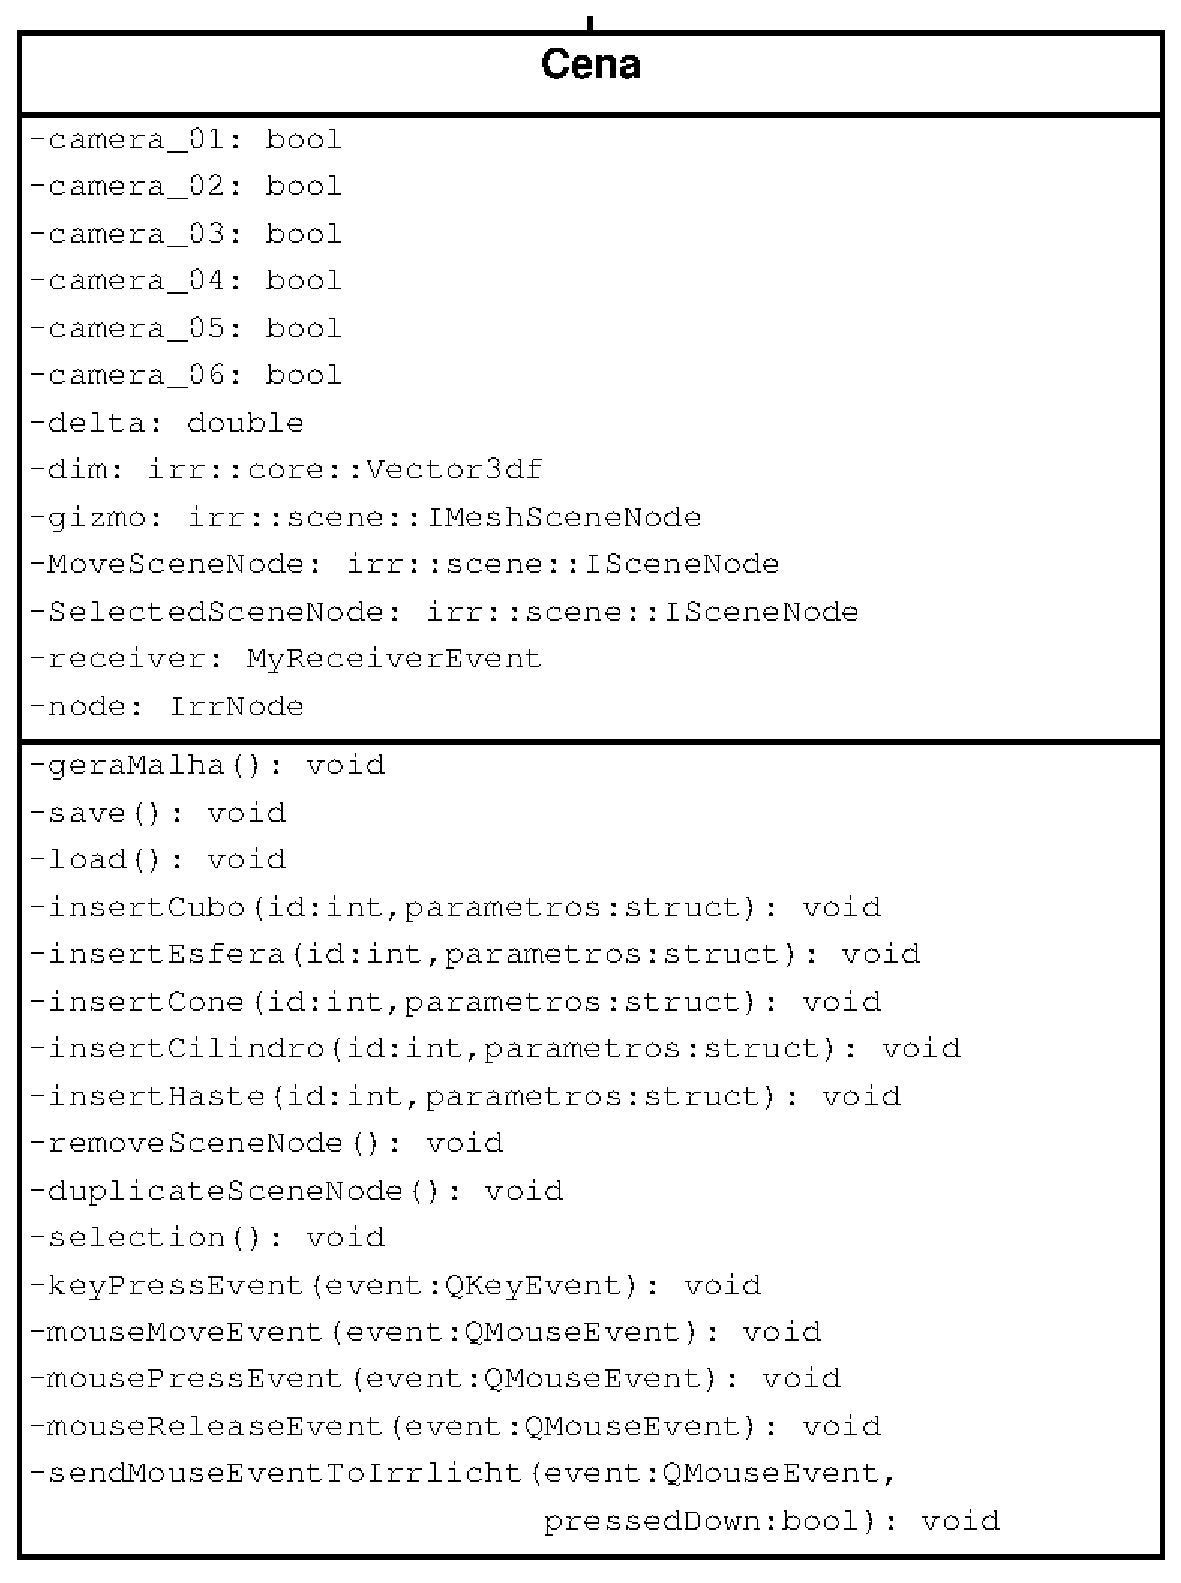
\includegraphics[scale = 0.4]{classecena}
	\caption{Classe Cena.}
	\label{fg:classecena}
\end{figure}

	Por fim, temos a classe \textit{MainWindow}, que utiliza-se de um objeto da classe \textit{Cena} para comunicar as alterações realizadas na interface com a janela {Irrlicht} e vice-versa. Desta forma, fazendo o tratamentos dos eventos de botão, mudança nos valores  dos  painéis laterais e dos campos de posição e rotação. A Figura~\ref{fg:classemainwindow} mostra os principais atributos e métodos deste classe.
\begin{figure}[!ht]
	\centering
	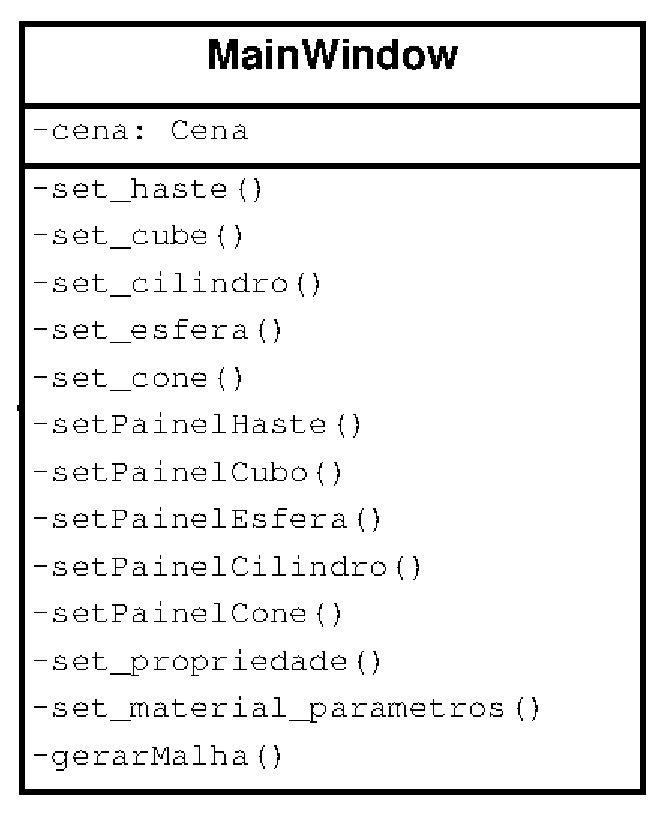
\includegraphics[scale = 0.4]{classemainwindow}
	\caption{Classe \textit{Mainwindow}.}
	\label{fg:classemainwindow}
\end{figure}

\section{Interface}
	O software desenvolvido neste projeto está ilustrado na Figura~\ref{fg:layout}. Seu layout e suas ferramentas foram baseada nos softwares de modelagem mais utilizados no mercado, que são: Blender, 3DStudio e Maya. A sua estrutura foi dividida em 4 áreas: barra superior, janela da cena, painéis laterais e barra inferior.
\begin{figure}[!ht]
	\centering
	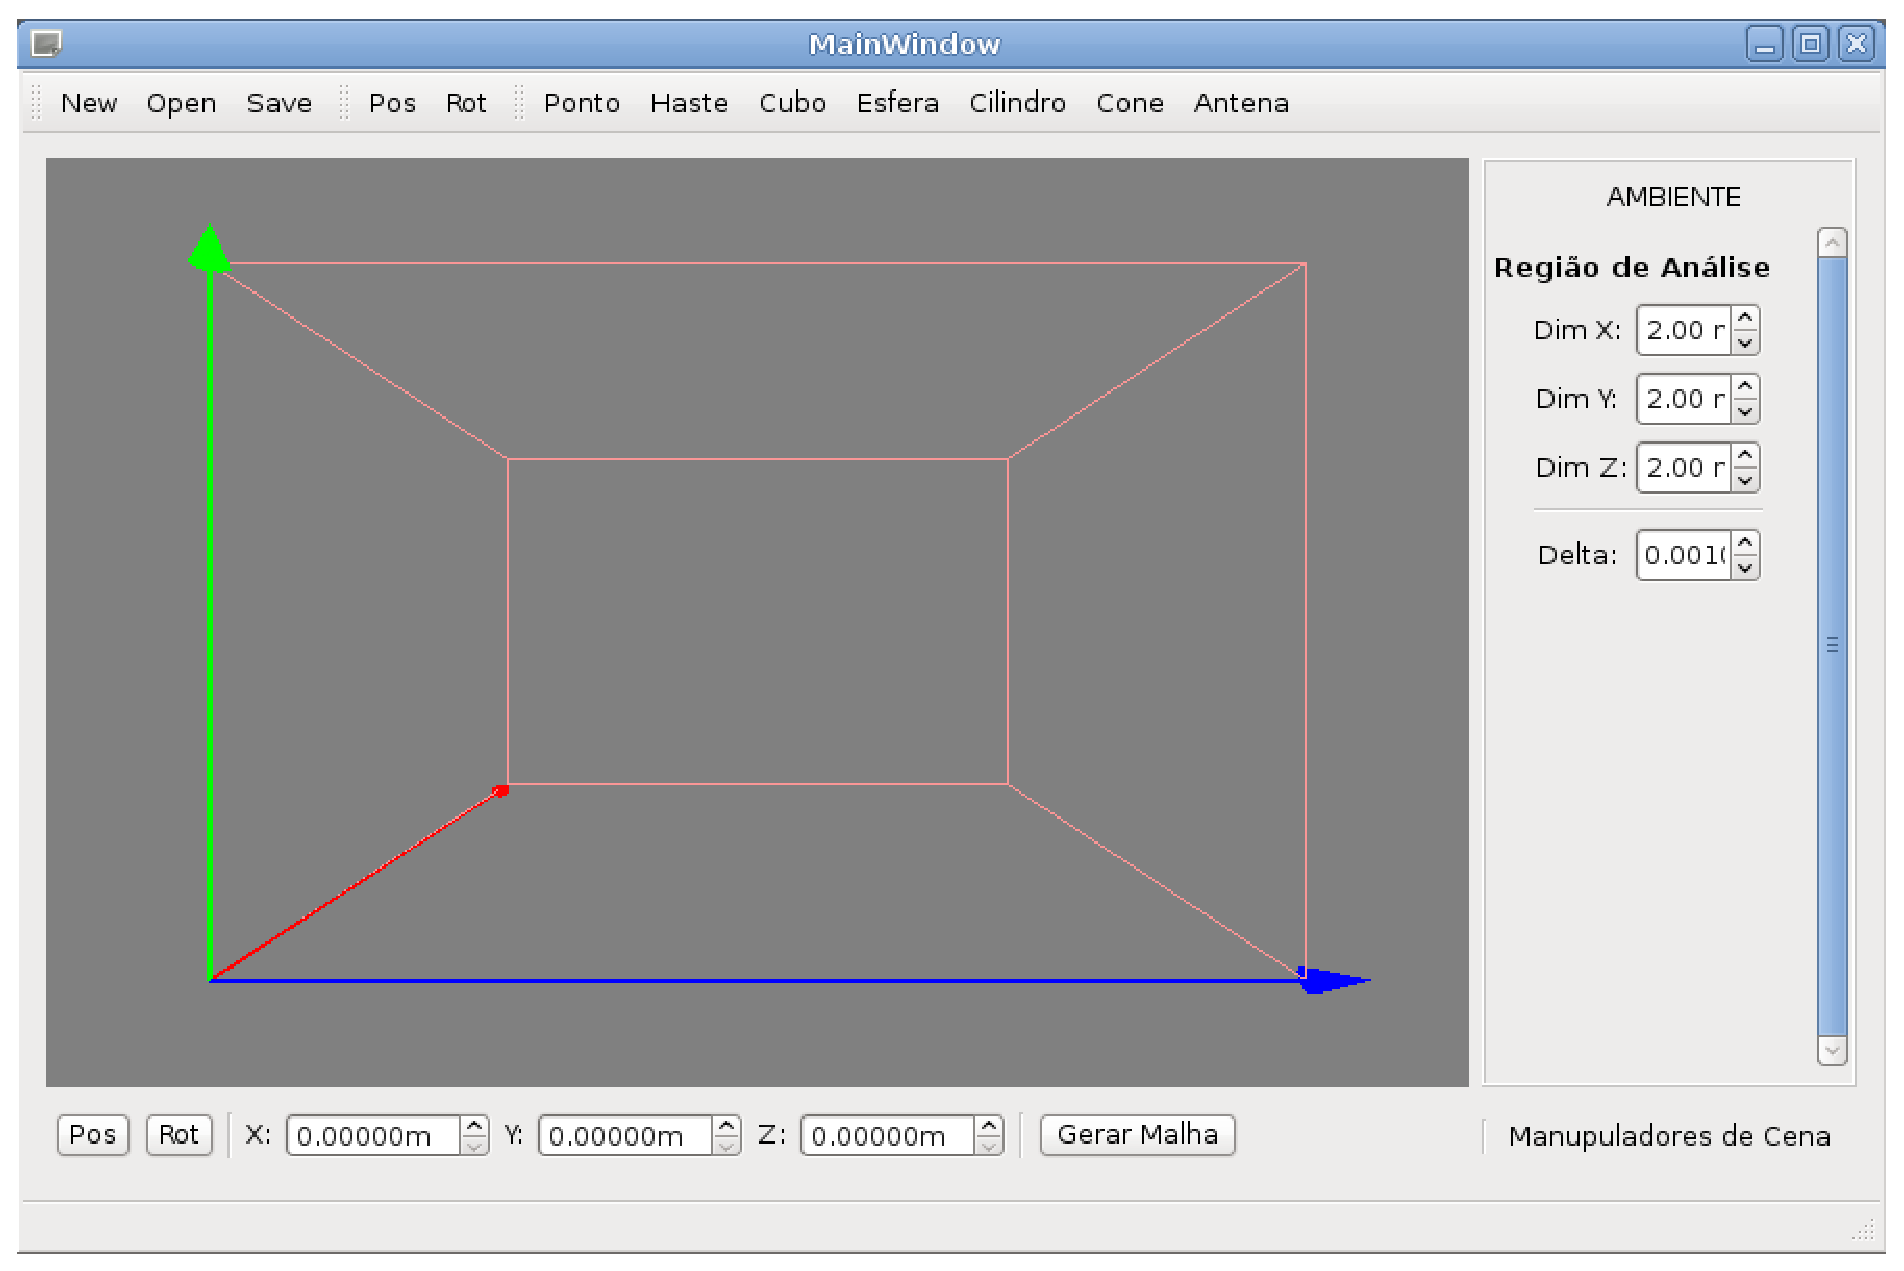
\includegraphics[scale = 0.4]{layout}
	\caption{Layout da interface.}
	\label{fg:layout}
\end{figure}

	Na barra superior, Figura~\ref{fg:barra_s}, encontra-se primeiramente o botão \textit{New}, que tem o propósito de criar uma nova cena \textit{Irrlicht}. Quando pressionado, ativa uma janela (Figura~\ref{fg:dados_r}) que requisita os dados necessários para criação da região de análise, tais como valores de dimensionamento (tamanho em $x$, $y$ e $z$) e o valor do $delta$ (dimensão da célula de Yee). Em seguida vem o botão \textit{Open}, que carrega uma cena anteriormente salvada (caso exista). Depois dele tem-se o botão \textit{Save}, que salva a cena atual em uma arquivo chamado \textit{Map.in}, que contém todas as características dos objetos (tamanho, tipo e parâmetros físicos), assim como suas posições.

\begin{figure}[!ht]
	\centering
	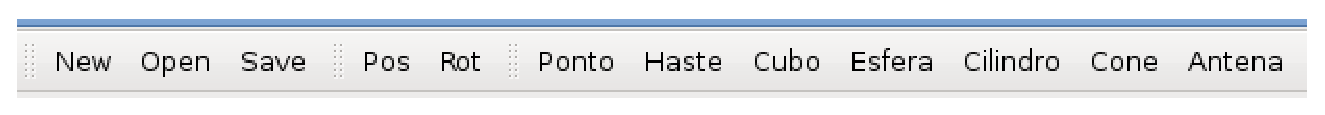
\includegraphics[scale = 0.4]{barra_s}
	\caption{Barra Superior interface.}
	\label{fg:barra_s}
\end{figure}
\begin{figure}[!ht]
	\centering
	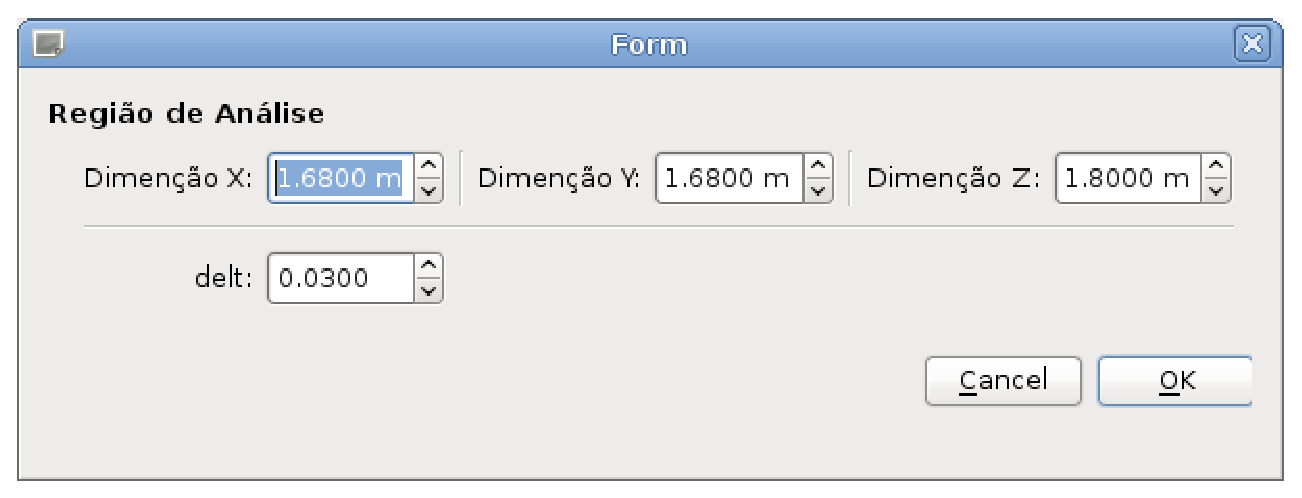
\includegraphics[scale = 0.4]{dados_r}
	\caption{Janela com as característica da região de análise.}
	\label{fg:dados_r}
\end{figure}

	Mas em frente, encontram-se os botões \textit{Pos} e \textit{Rot}, os quais dão suporte à visualização e manipulação do posicionamento e dos ângulos de cada objeto selecionado, respectivamente. Logo em seguida encontram-se os criadores de objetos básico da interface, que são \textit{Ponto},\textit{Haste}, \textit{Cubo}, \textit{Esfera}, \textit{Cilindro}, \textit{Cone} e por fim \textit{Antena}. Quando ativados criam o objeto desejado com a posição e os parâmetros previamente especificados.

	A janela da cena, Figura~\ref{fg:janela_c} é uma região do software onde se visualiza o universo virtual. Nesta região, é possível realizar manipulações através do mouse como seleção, translação e rotação. Ela está diretamente relacionada a classe \textit{IrrViewer}, pois é uma instância (objeto) desta classe. 

\begin{figure}[!ht]
	\centering
	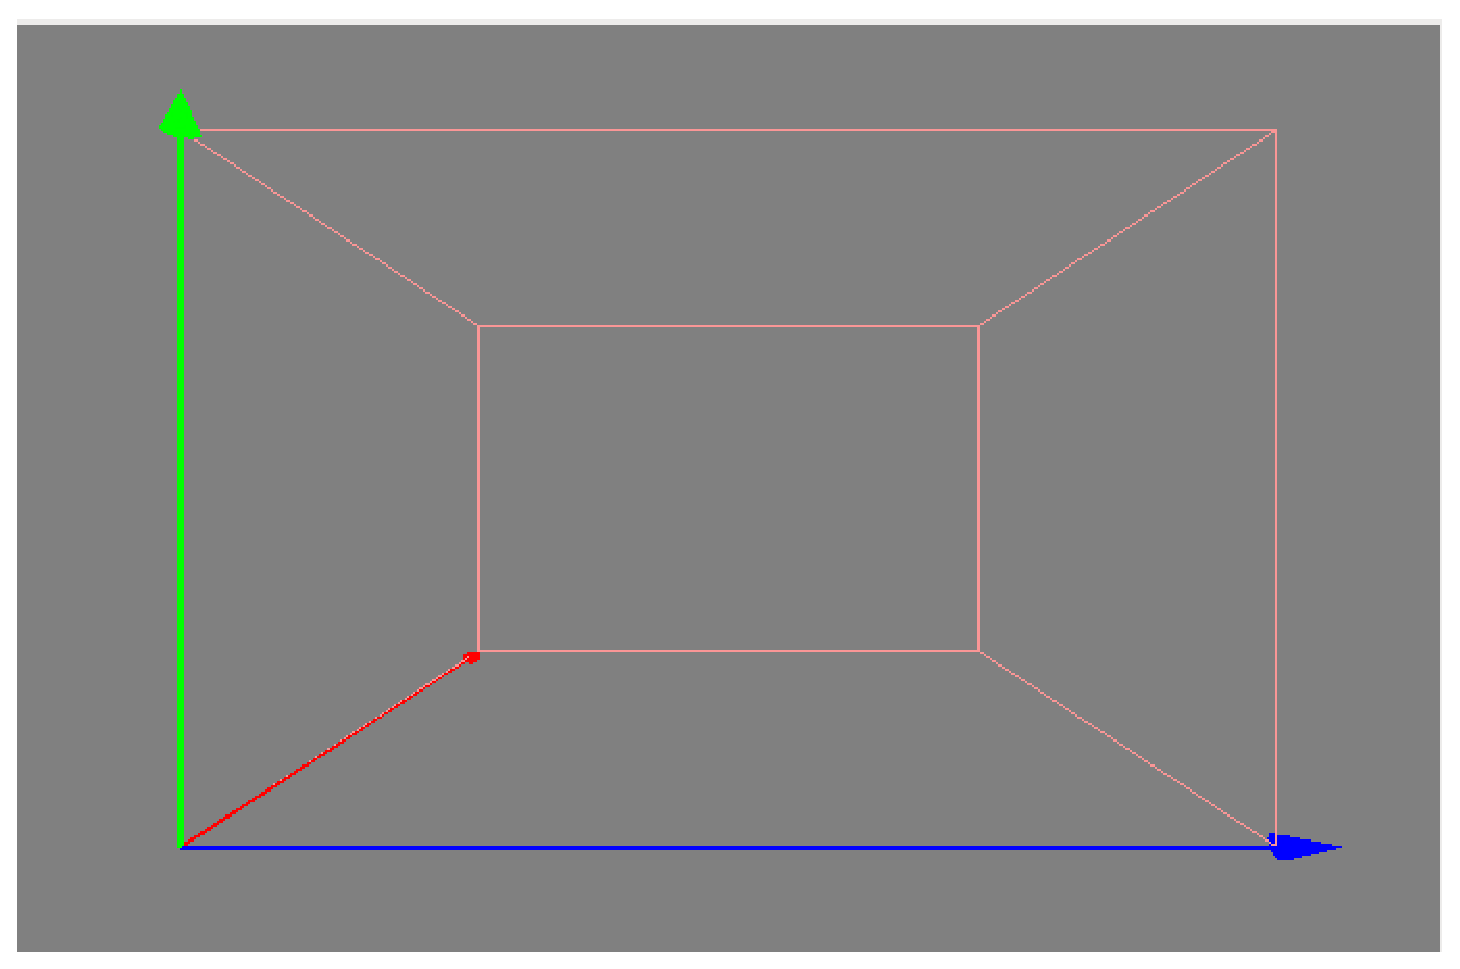
\includegraphics[scale = 0.4]{janela_c}
	\caption{Janela da Cena.}
	\label{fg:janela_c}
\end{figure}

	O painel lateral, Figura~\ref{fg:painel_l} é uma área de visualização e manipulação das características relacionadas ao tamanho e parâmetros físicos dos objetos.

\begin{figure}[!ht]
	\centering
	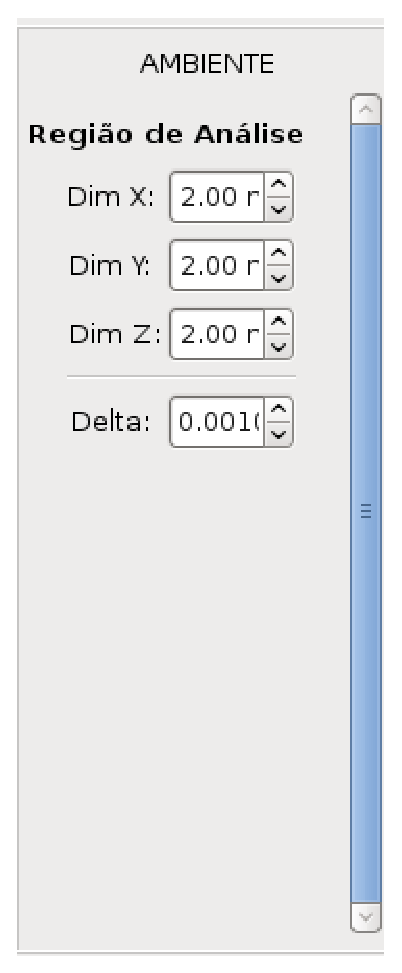
\includegraphics[scale = 0.4]{painel_l}
	\caption{Painel lateral dos parâmetros da região de análise.}
	\label{fg:painel_l}
\end{figure}

	Na parte inferior da interface(Figura~\ref{fg:barra_i}) encontram-se os botões \textit{Pos} e \textit{Rot}, que têm as mesmas funcionalidades dos já citados da barra superior. Em seguida  há um conjunto de itens que possibilitam a visualização e manipulação das coordenadas relativas a posição e rotação do objeto selecionado ($X$, $Y$ e $Z$). E por fim, o botão \textit{gerar Malha}, o qual tem a função de gerar e salvar a malha representativa de todos os  objetos construídos no cenário virtual.

\begin{figure}[!ht]
	\centering
	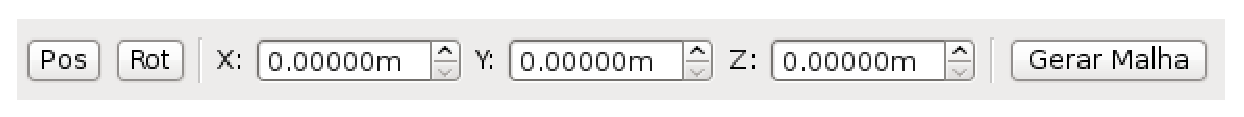
\includegraphics[scale = 0.4]{barra_i}
	\caption{Barra inferior da interface.}
	\label{fg:barra_i}
\end{figure}

\section{Funcionalidades}
	\subsection{Atalhos de Teclado}
	A facilidade de navegação e manipulação, são características fundamentais para qualquer software de modelagem. Os atalhos de teclado são criados com o intuito de reduzir esforço e tempo do usuário. Esta ferramenta é um conjunto de teclas que ao serem pressionadas realizam uma ação. As ações realizadas pelas teclas de atalho, normalmente podem ser realizada por outras ferramentas como botões, menus, etc.
	
	A Tabela~\ref{tb:shortcuts} contém todos os atalhos de teclado criados para este projeto.

\begin{table}
\centering
\begin{tabular}{|l|l|}
	\hline
		Atalho & Funcionalidade \\ \hline
		Shift+O &  Afastamento\\ \hline
		Shift+P &  Aproximação\\ \hline
		W & Focaliza objeto selecionado\\ \hline
		C & Clona objeto selecionado(duplica)\\ \hline
		R & Remove objeto selecionado \\ \hline
		1 & Muda para câmera frente \\ \hline
		2 & Muda para câmera lateral esquerda \\ \hline
		3 & Muda para câmera lateral direita \\ \hline
		4 & Muda para câmera traseira \\ \hline
		5 & Muda para câmera topo \\ \hline
		6 & Muda para câmera base \\ \hline
		M + X & Permite movimentação de objeto selecionado no eixo X com o mouse \\ \hline
		M + Y & Permite movimentação de objeto selecionado no eixo Y com o mouse \\ \hline
		M + Z & Permite movimentação de objeto selecionado no eixo Z com o mouse \\ \hline
		Shift + A & Permite movimentação de objeto selecionado nos eixos X e Y com o mouse \\ \hline
		Shift + B & Permite movimentação de objeto selecionado nos eixos X e Z com o mouse \\ \hline
		Shift + C & Permite movimentação de objeto selecionado nos eixos Y e Z com o mouse \\ \hline
		Shift + D & Permite movimentação de objeto selecionado nos eixos X, Y e Z com o mouse \\ 
	\hline
\end{tabular}
\caption{Tabela de Atalhos de teclado.}
\label{tb:shortcuts}
\end{table}
	
\subsection{Eventos de Colisão}
\label{sec:colisao}
	Os eventos de colisão possibilitam que duas ou mais formas geométrica existentes no AV possam colidir.  Neste trabalho utilizou-se a colisão por reta, que é ortogonal ao plano de visualização da câmera. Seu ponto inicial fica posicionado no centro ecrã (tela), já seu o ponto final é deslocado do inicial por uma distância consideravelmente maior do que qual uma das arestas da região de análise. Este ponto final responde ao evento de \textit{mouse}, ou seja, no caso da ocorrência de um \textit{click}  em um determinado ponto do cenário 3D a reta de colisão terá o seu ponto inicial recebendo o valor central da tela e o final obtendo o valor da posição do \textit{mouse}.  No caso de esta reta encontrar (colidir) algum objeto entre seus pontos ele será o objeto selecionado. 
 
	Para diferenciar, visualmente, objetos selecionados dos não selecionados, utilizou-se da técnica de representação \textit{wireframe}. Portanto, quando ocorrer um evento de colisão e um objeto é selecionado, a visualização deste objeto muda, passando a ser representado somente por suas arestas e vértices. A Figura~\ref{fg:colision} demostra este fato.
\begin{figure}[!ht]
	\centering
	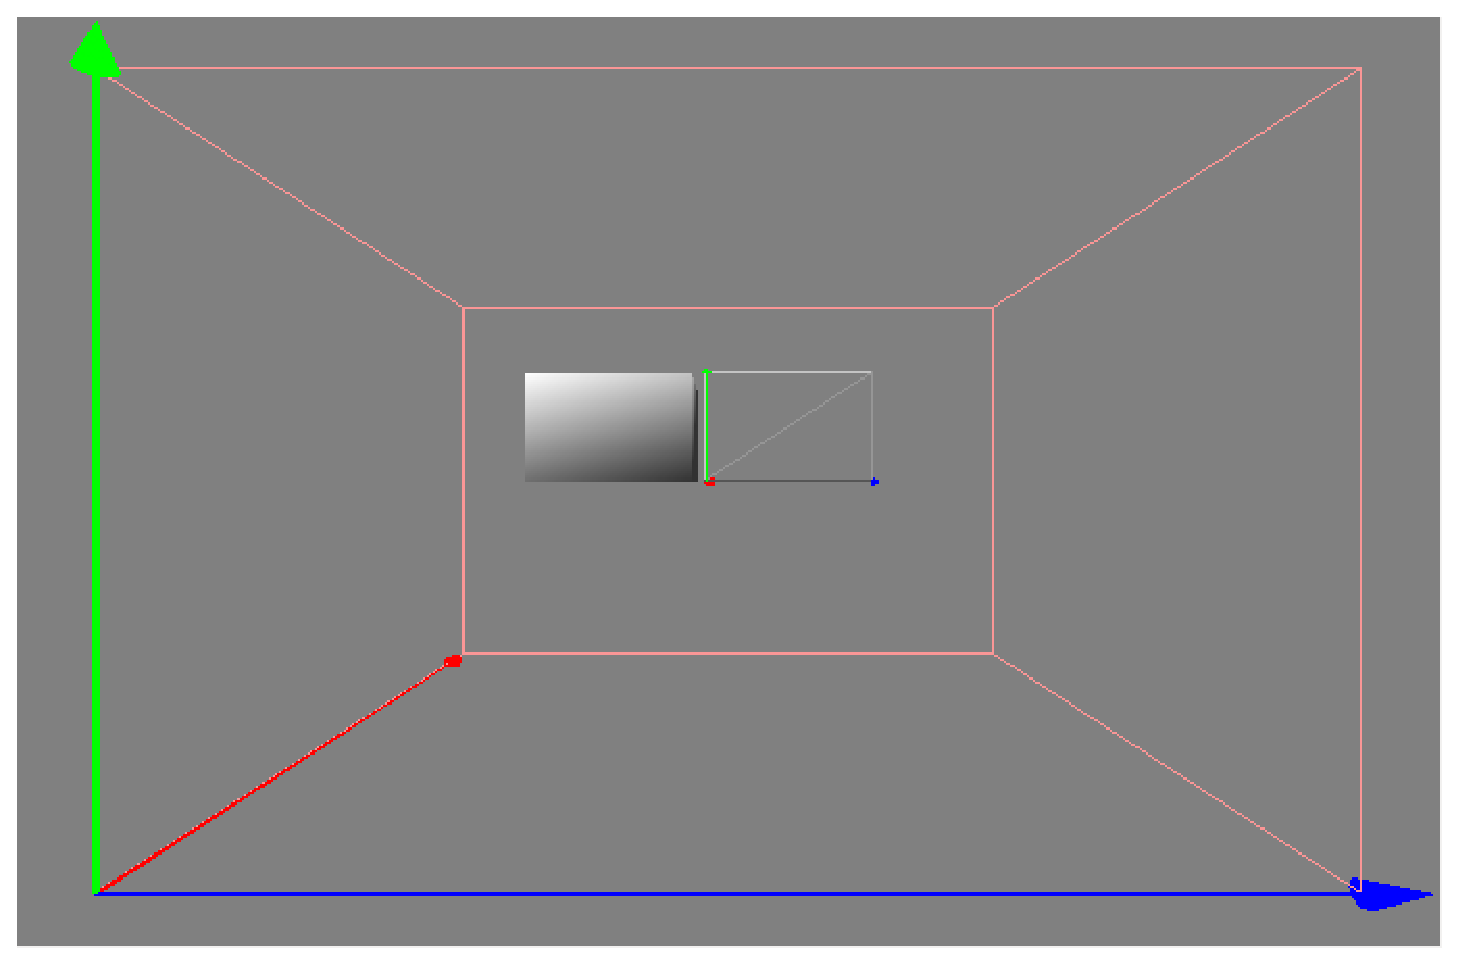
\includegraphics[scale = 0.4]{colision}
	\caption{Ilustração do evento de colisão com o objeto cubo.}
	\label{fg:colision}
\end{figure}

\subsection{Visualizações}
	A possibilidade de visualização de um cenário por vários ângulos é fundamental quando se está modelando um ambiente 3D, principalmente quando o cenário modelado será utilizado em simulações eletromagnéticas, onde qualquer erro estrutural poderá gerar resultados não desejados (sem sentido). Para sanar esse problema, o software confeccionado neste projeto, permiti visualizar o AV por seis câmeras diferentes: frontal(padrão), lateral esquerda, lateral direita, traseira, topo e base. 

\subsection{Aproximação e Afastamento}
	Tem a finalidade de, juntamente com as seis visualizações possíveis(seis câmeras diferentes), facilitar a navegação e alteração do cenário virtual. Sendo uma ferramenta importante na modelagem, por permitir a aproximação e afastamento de um determinado região ou objeto selecionado dentro do ambiente virtual. As teclas de atalho associadas a aproximação são $Shift+P$ ou $W$ e as associadas aos afastamento são $Shift+O$.

	As figuras a seguir ilustram o uso desta ferramenta. A Figura~\ref{fg:nor} mostra um objeto a uma distância padrão (sem afastamento ou aproximação). Na Figura~\ref{fg:afas} pode ser visto o mesmo objeto após um determinado afastamento (utilizando $Shift+O$). Já as Figuras~\ref{fg:apr} e \ref{fg:w} mostra os efeitos da  aproximação normal (usando o atalho $Shift+P$) e a por seleção (dada pela tecla $W$).

\begin{figure}[!ht]
	\begin{center}
		\subfigure[Visualização de objeto cilindro sem aproximação, afastamento ou mudança de foco da câmera.]{\label{fg:nor}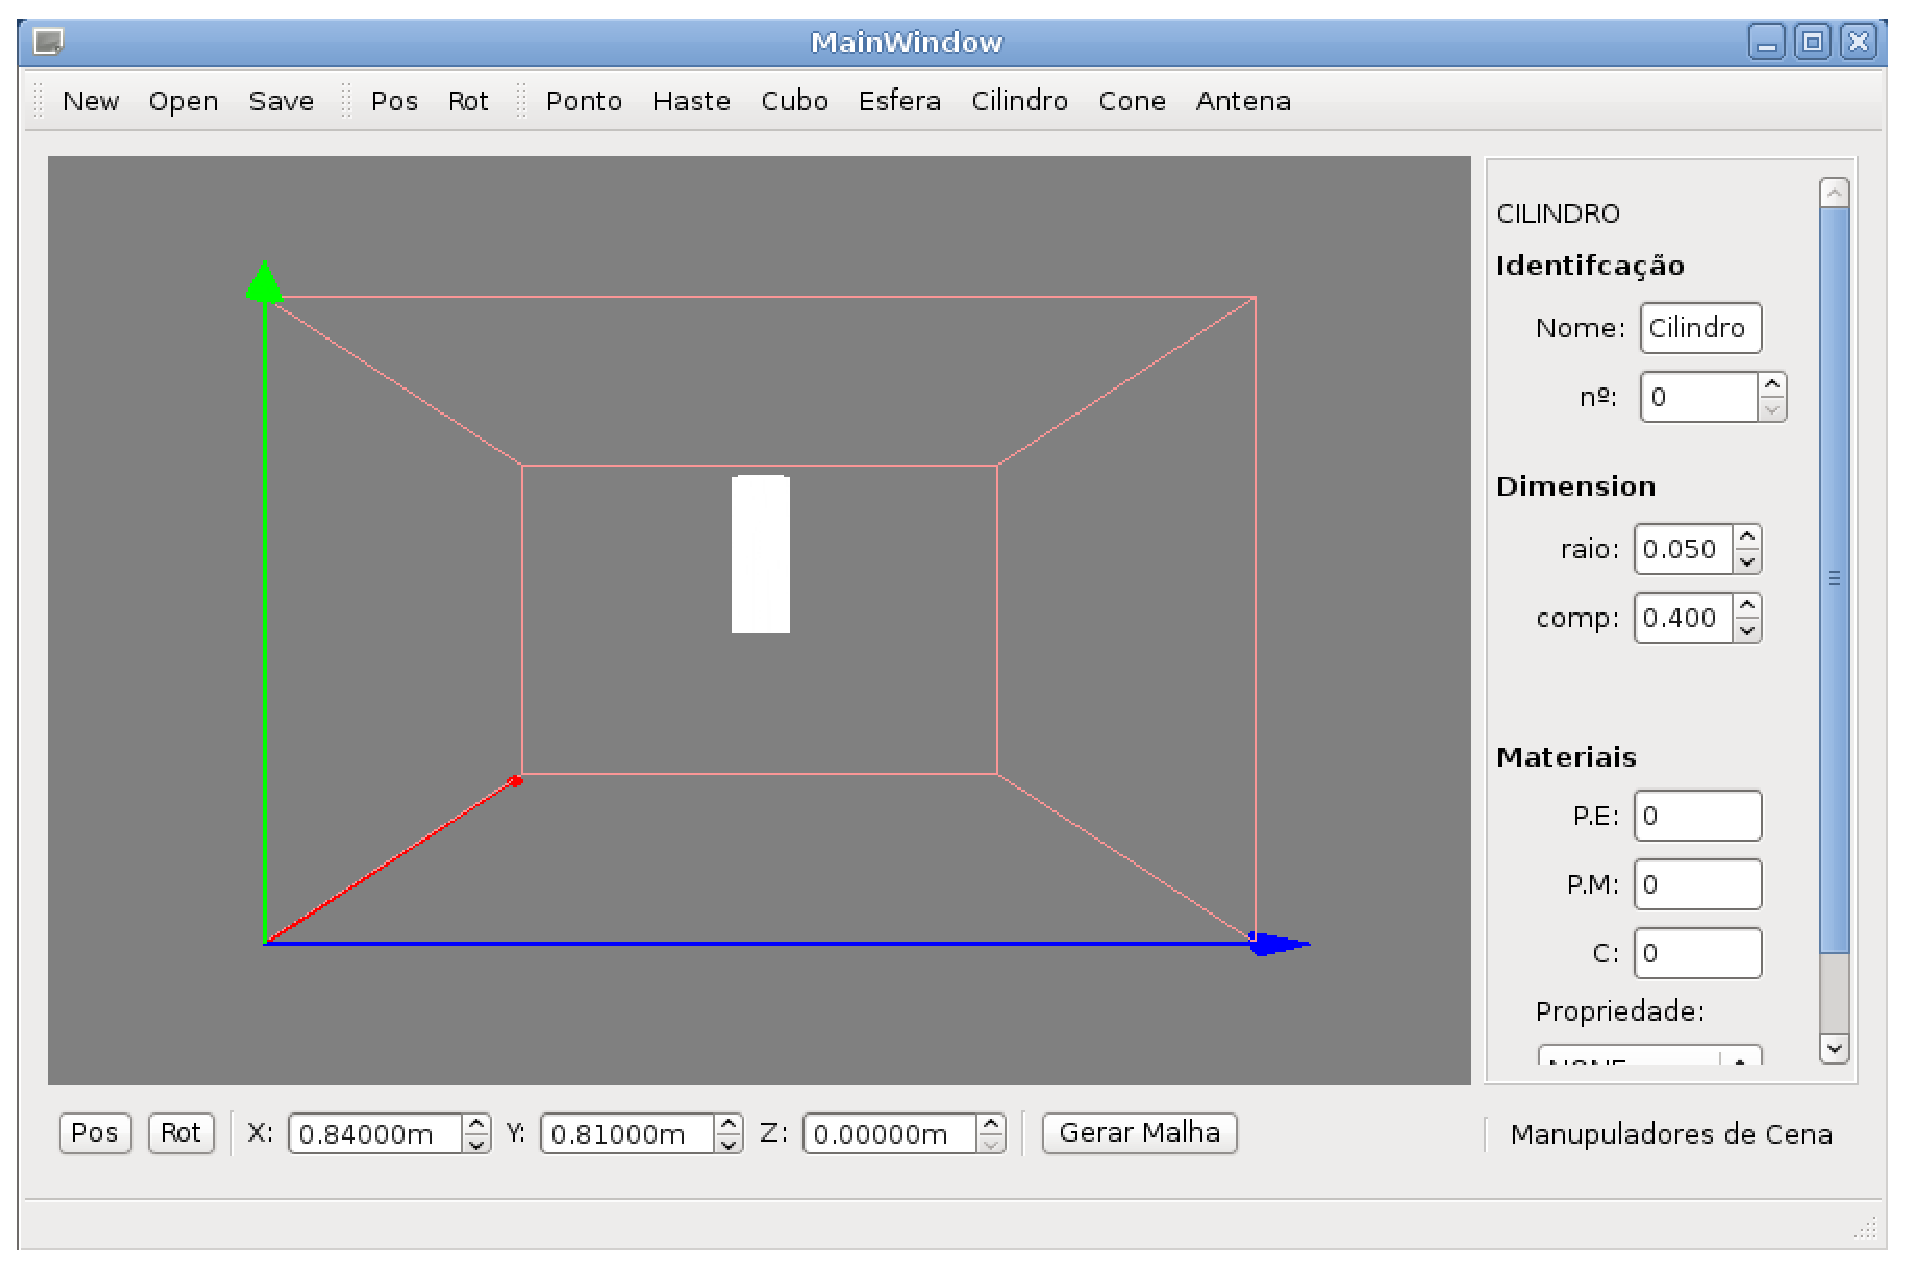
\includegraphics[scale=0.25]{nor}}
\qquad
		\subfigure[Visualização de objeto cilindro com afastamento.]{\label{fg:afas}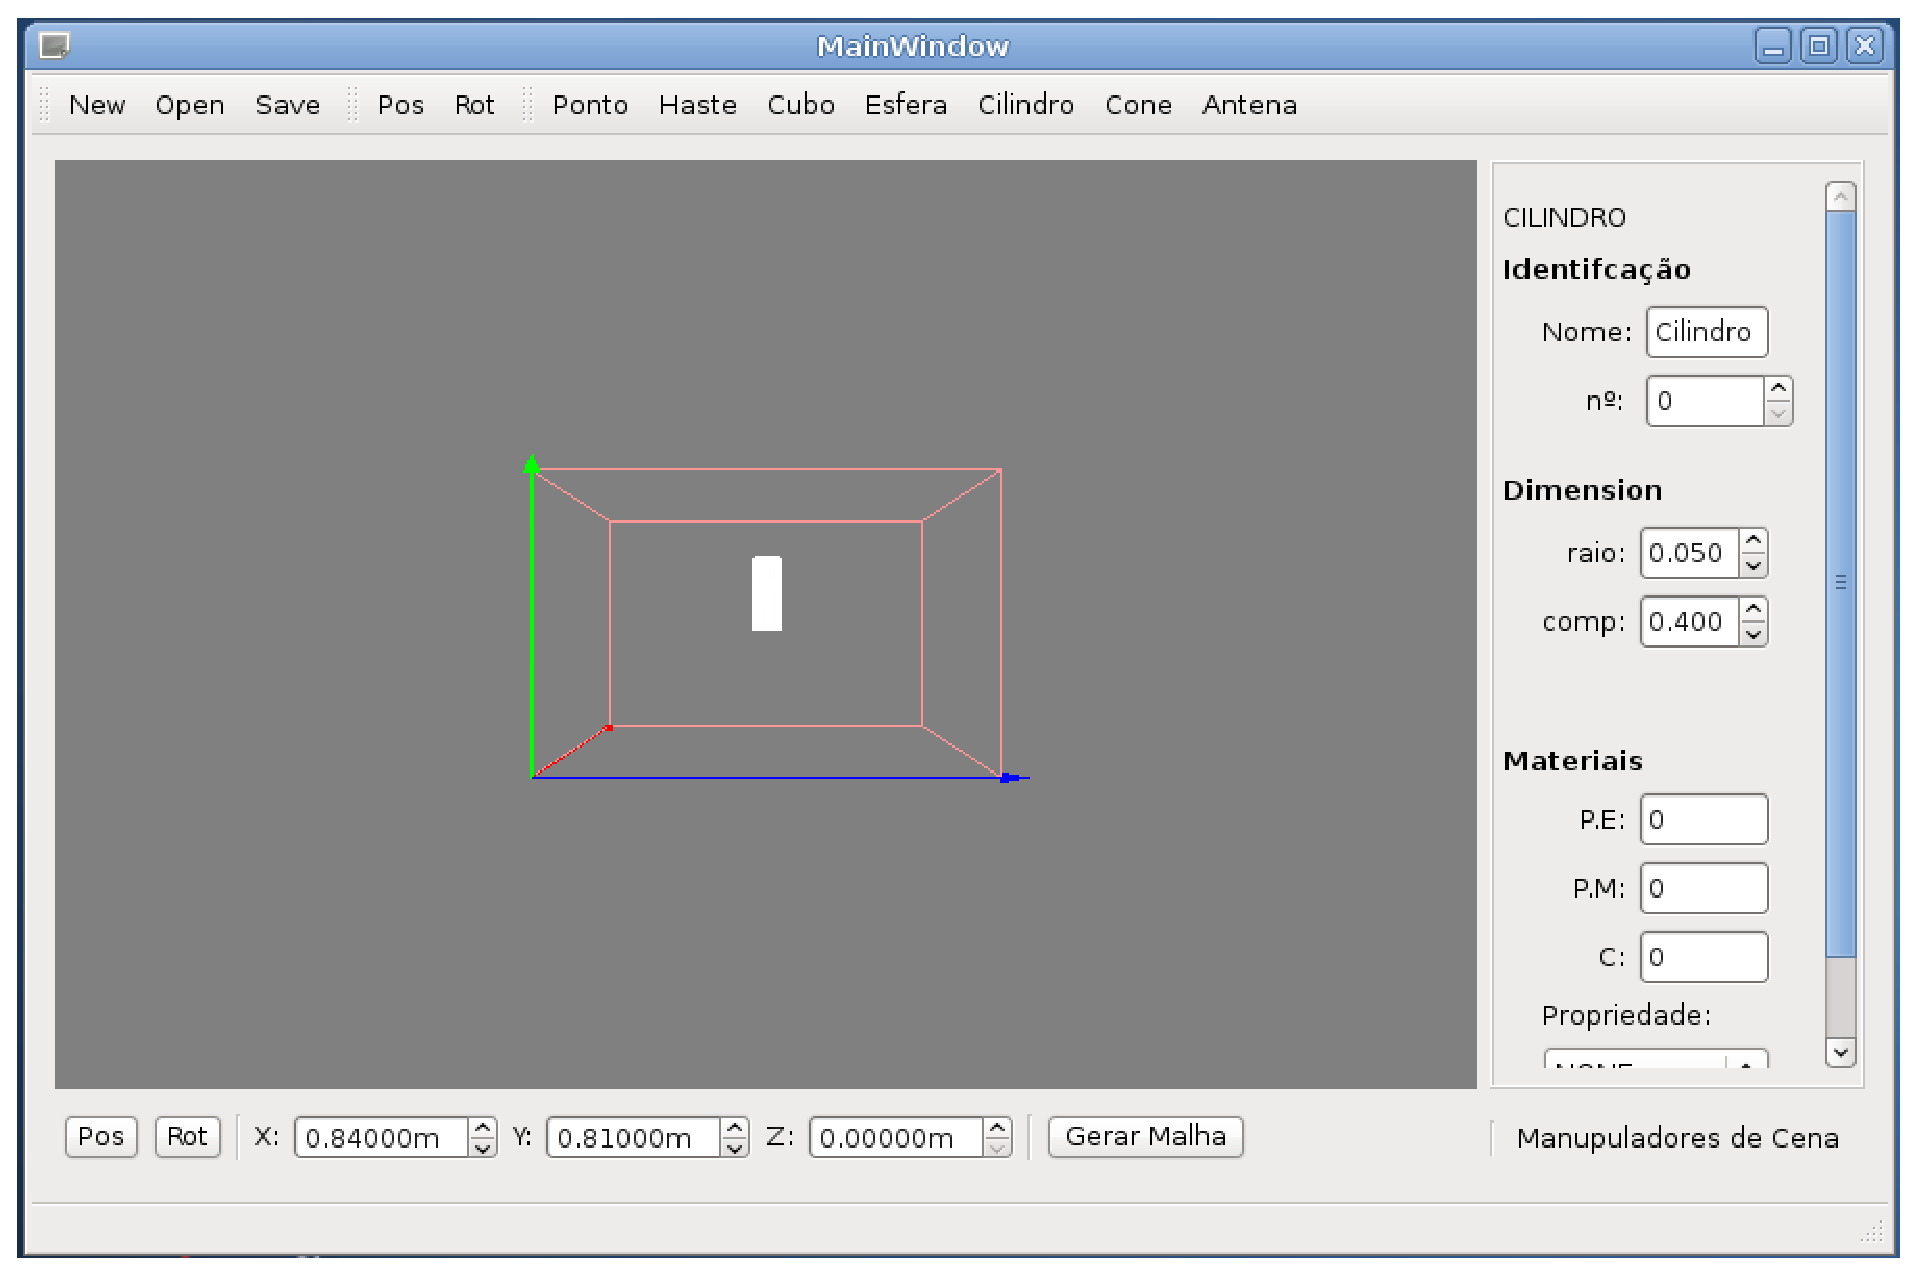
\includegraphics[scale=0.25]{afas}}
	\end{center}
	\caption{Visualização por afastamento.}
	\label{fg:afastamento}
\end{figure}

\begin{figure}[!ht]
	\begin{center}
		\subfigure[[Visualização de objeto por aproximação normal(sem mudança de foco).]{\label{fg:apr}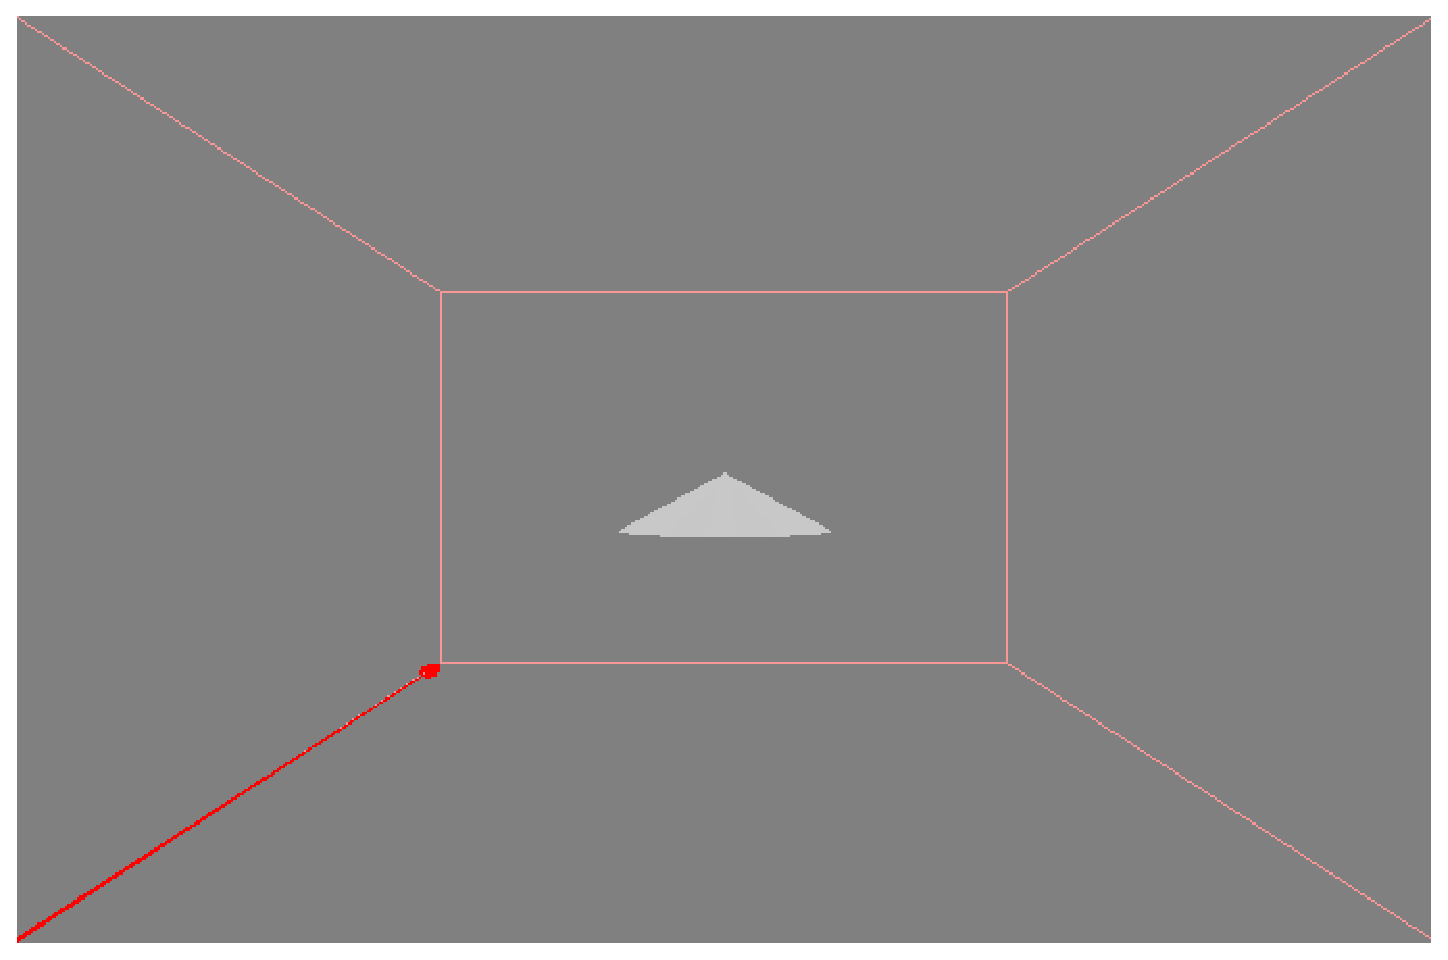
\includegraphics[scale=0.25]{apr}}
\qquad
		\subfigure[Focalização de objeto selecionado através da tecla $W$.]{\label{fg:w}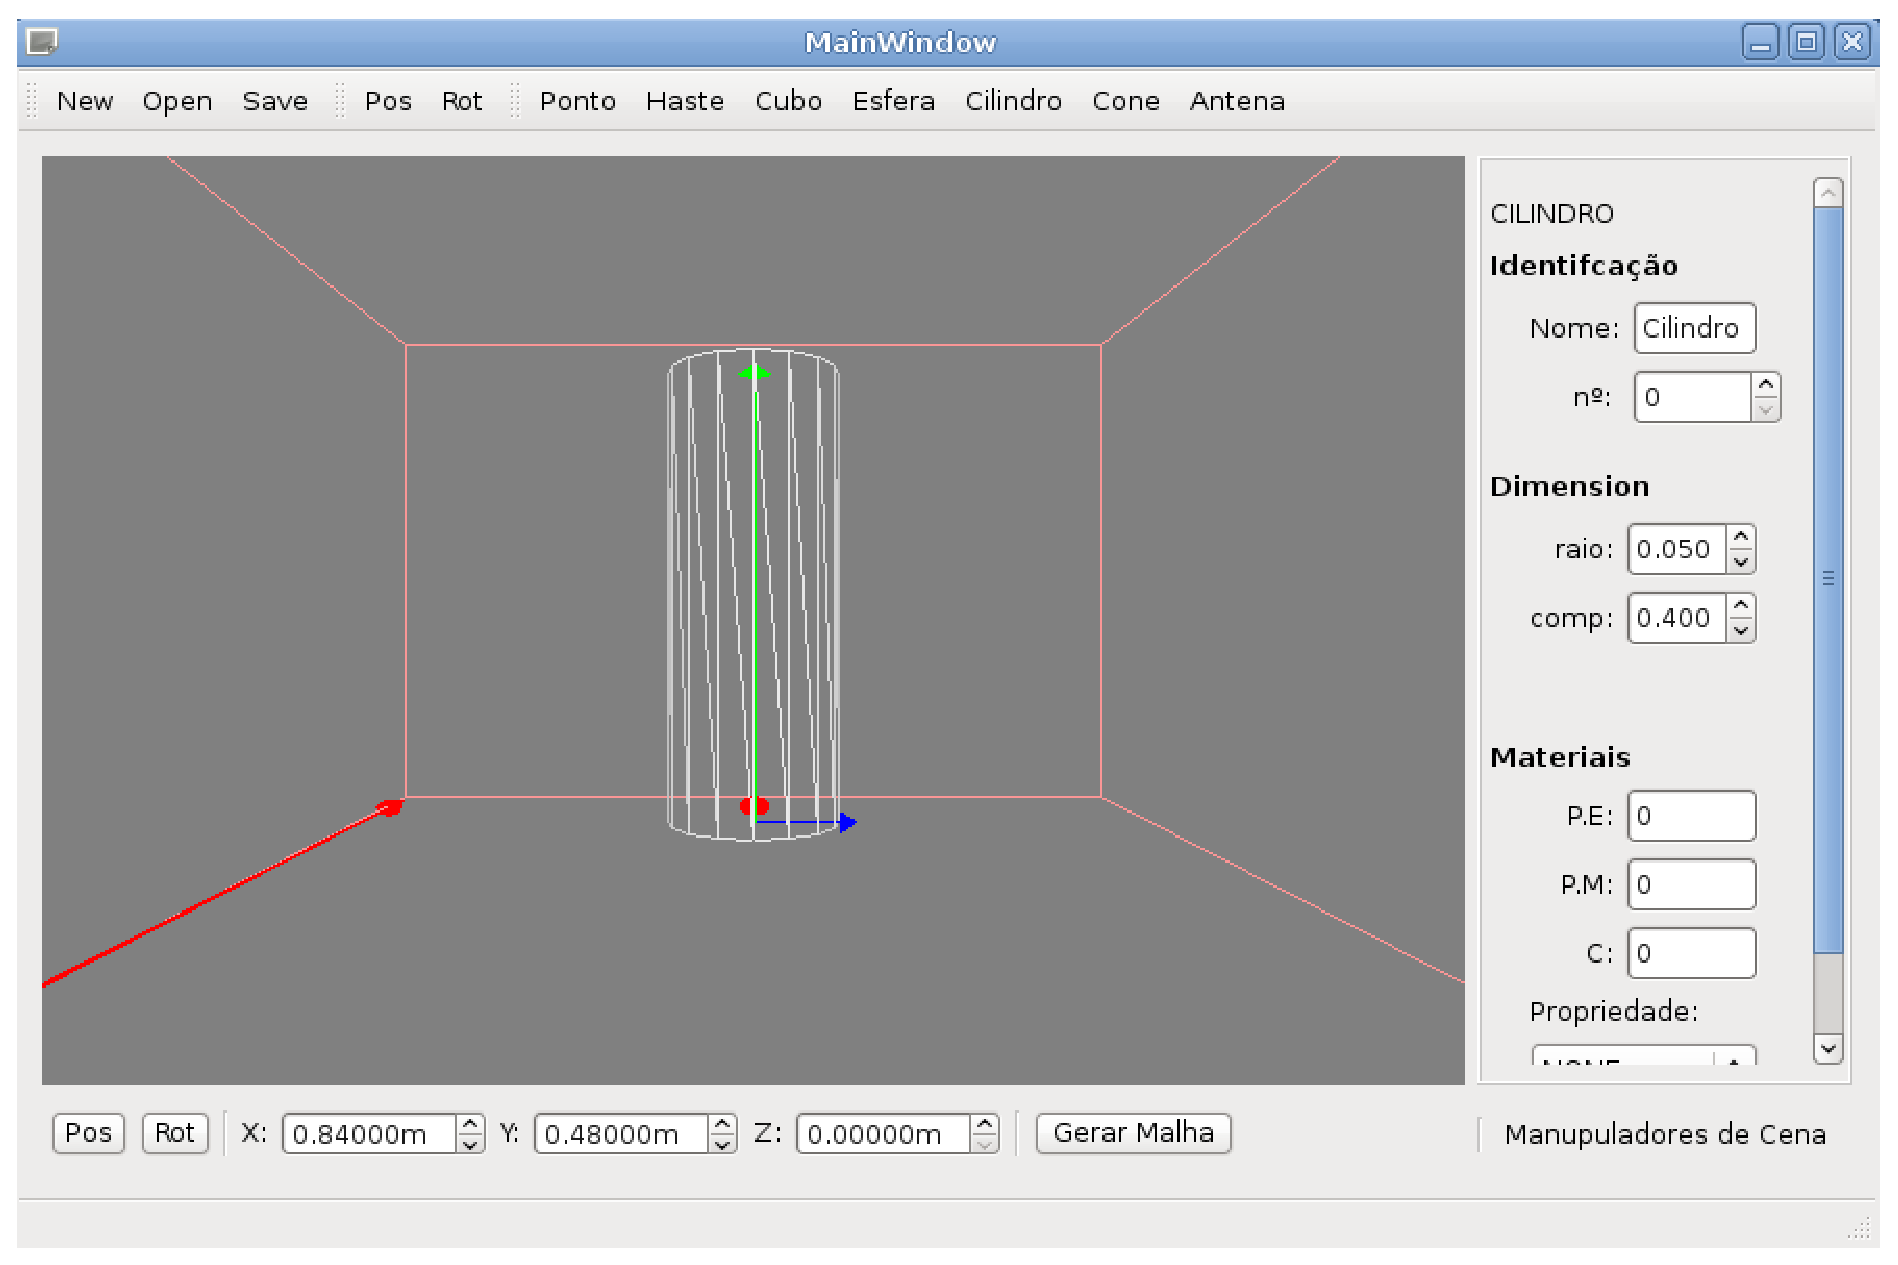
\includegraphics[scale=0.25]{w}}
	\end{center}
	\caption{Visualização por aproximação.}
	\label{fg:aproximacao}
\end{figure}

\subsection{Conexão com o LANE-SAGS}
\label{sec:c_sags}
	Depois de implementar todas as funcionalidades do software, passou-se para o último requisito proposto para este projeto, a conexão com o simulado LANE-SAGS. Esta conexão foi realizada por meio de dois arquivos.

	O primeiro arquivo é o bd.in (bd - bloco dielétrico), que contém os prismas retangulares (células) que representam, por enumeração de ocupação espacial, os objetos contínuos modelados na interface. A sequência de gravação de cada prismas no arquivo segue a forma: célula inicial $X$, célula final $X$, célula inicial $Y$, célula final $Y$, célula inicial $Z$, célula final $Z$, $\epsilon_r$, $\sigma$ e $\mu_r$.
 Além do arquivo bd.in, é gerado um segundo arquivo chamado \textit{simconf.in}(simconf- configuração da simulação) contendo as informações referentes às: dimensões das células de Yee (em metros) e a dimensão em células do Espaço Delimitador (região de análise).
Com os arquivos gerados e a conexão estabelecida, basta inserir (utilizando o LANE-SAGS) alguns fatores fundamentais para efetuar uma simulação de propagação eletromagnética, tais como: antena, planos de visualização, fonte e corrente. O diagrama mostrado na Figura \ref{fg:c_sags}, ilustra o processo de execução de uma simulação utilizando os dois softwares.

\begin{figure}[!ht]
	\centering
	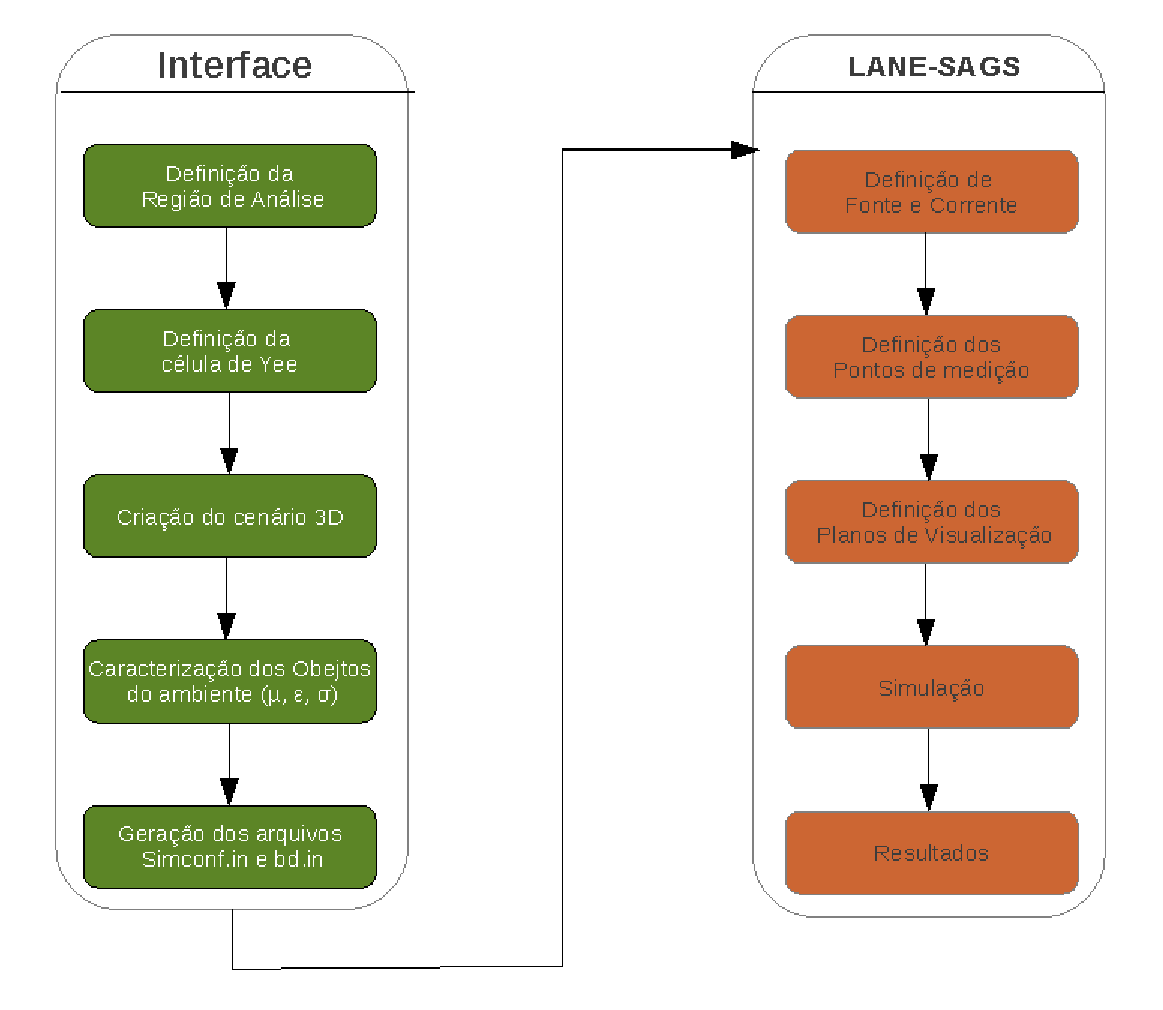
\includegraphics[scale = 0.8]{c_sags}
	\caption{Diagrama de conexão com o LANE-SAGS.}
	\label{fg:c_sags}
\end{figure}


\chapter{Aplicação e Resultados}
%Com a finalidade de validar a interface, foi construído um AV apartir da caracteristicas de um ambiente real(escritório), com planta baixa ilustrada na Figura~\ref{fg:planta_baixa}. Através de uma antena, foram feitas medições nesse ambiente (sempre mantendo a porta fechada), o que possibilitou capturar as caracteristicas físicas dos objetos presentes assim como a resposta desse ambiente a propagação do sinal dessa antena.\\

\begin{figure}[ht!]
	\centering
	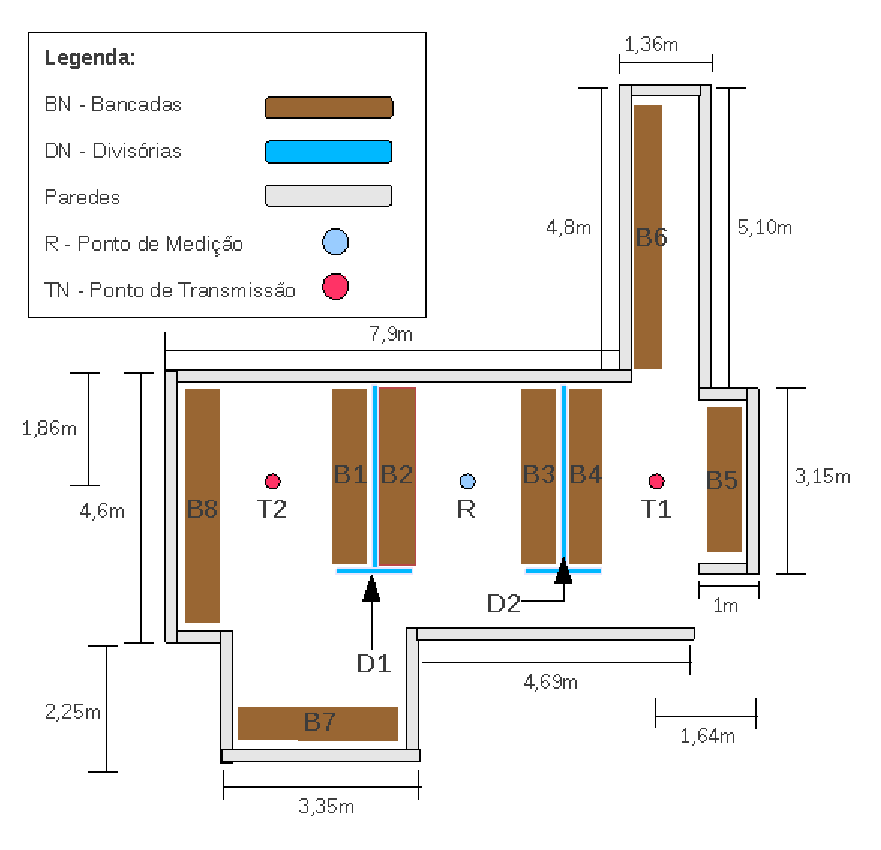
\includegraphics[scale = 1]{planta_baixa}
	\caption{Planta baixa do escritório modelado usando a interface.}
	\label{fg:planta_baixa}
\end{figure}

Todos os objetos presentes na hora das medições foram modelados, sendo eles: computadores, bancadas, monitores, divisórias e paredes divisórias. Suas dimensões estão especificada na Tabela~\ref{tb:objetos}.

\begin{table}
\centering
	\begin{tabular}{|l|l|l|l|}
	\hline
	\textbf{Objetos} & \textbf{Dimensão $X$} & \textbf{Dimensão} $Y$ & \textbf{Dimensão $Z$}\\ \hline
	Computadores (CPU's) & $0,18m$ & $0,43m$ & $0,42m$ \\ \hline
	Monitores & $0,39m$ & $0,31m$ & $0,39m$ \\ \hline
	Divisórias $1$ e $2$ & $3,27m$ & $1,5m$ & $0,03m$ \\ \hline
	Paredes divisórias $1$ e $2$ & $0,03m$ & $1,5m$ & $1m$ \\ \hline
	Bancadas de $1$-$4$ & $3,21m$ & $0,03m$ & $0,5m$ \\ \hline
	Bancada $5$ & $2,94m$ & $0,03m$ & $0,5m$ \\ \hline
	Bancada $6$ & $4,68m$ & $0,03m$ & $0,5m$ \\ \hline
	Bancada $7$ & $0,5m$ & $0,03m$ & $3,18m$ \\ \hline
	Bancada $8$ & $4,26m$ & $0,03m$ & $0,5m$ \\
	\hline
	\end{tabular}
	\caption{Objetos e suas dimensões.}
	\label{tb:objetos}
\end{table}

Alguns desse objetos estão dispostos em alturas diferentes em relação ao piso. As bancadas e o teto estão a uma altura de 0,75 metros e 2,73 metros, respectivamente. Os computadores e monitores foram colocados uma célula acima do nível das bancadas, como a altura das bancadas é de 25 células, eles foram modelados apartir da célula 26 (equivalente a uma altura de 0,78m).\\

As dimensões gerais desse cenário usadas na interface, foram:
\begin{itemize}
\item \textit{Delta}(Tamanho da célula de Yee) utilizada foi de $0,003m$.
\item \textit{Região de Análise} com dimensões: $X$ = $15m$, $Y$ = $3m$ e $Z$ = $15m$.
\item \textit A lista das carateristicas físicas com seus respectivos matérias estam presentes na Tabela~\ref{tab:materiais}
\end{itemize}

\begin{table}
\centering
	\begin{tabular}{|l|l|l|l|l|}
	\hline
	Elementos dos Ambiente & Material & $\epsilon$ & $\sigma$ & $\mu$ \\ \hline
	Parede & Tijolo & $4$ & $0,0135$ & $1$\\ \hline
	Teto & Gesso & $2,8$ & 0,1533 & 1 \\ \hline
	Bancadas & Madeira & $1,8$ & $0,011$ & $1$\\ \hline
	Monitores e Gabinetes & Metal & $5$ & $1\times10^{11}$ & $1$\\ \hline
	Divisórias & Vidro & $5$ & $5\times10^{-4}$ & $1$ \\ \hline
	Piso & Concreto & $5$ & $1$ & $1$ \\
	\hline
	\end{tabular}
	\caption{Tabela de elemetos, materiais parâmetros físicos.}
	\label{tab:materiais}
\end{table}

Como resultado da modelagem usando a interface, obeteve-se a estrutura mostrada na Figura(colocar figura estrutura da interface). A disposição dos seus objetos tentou seguir o posicionamento real dos mesmos no momento das medições.

%\begin{figure}[ht!]
%	\centering
%	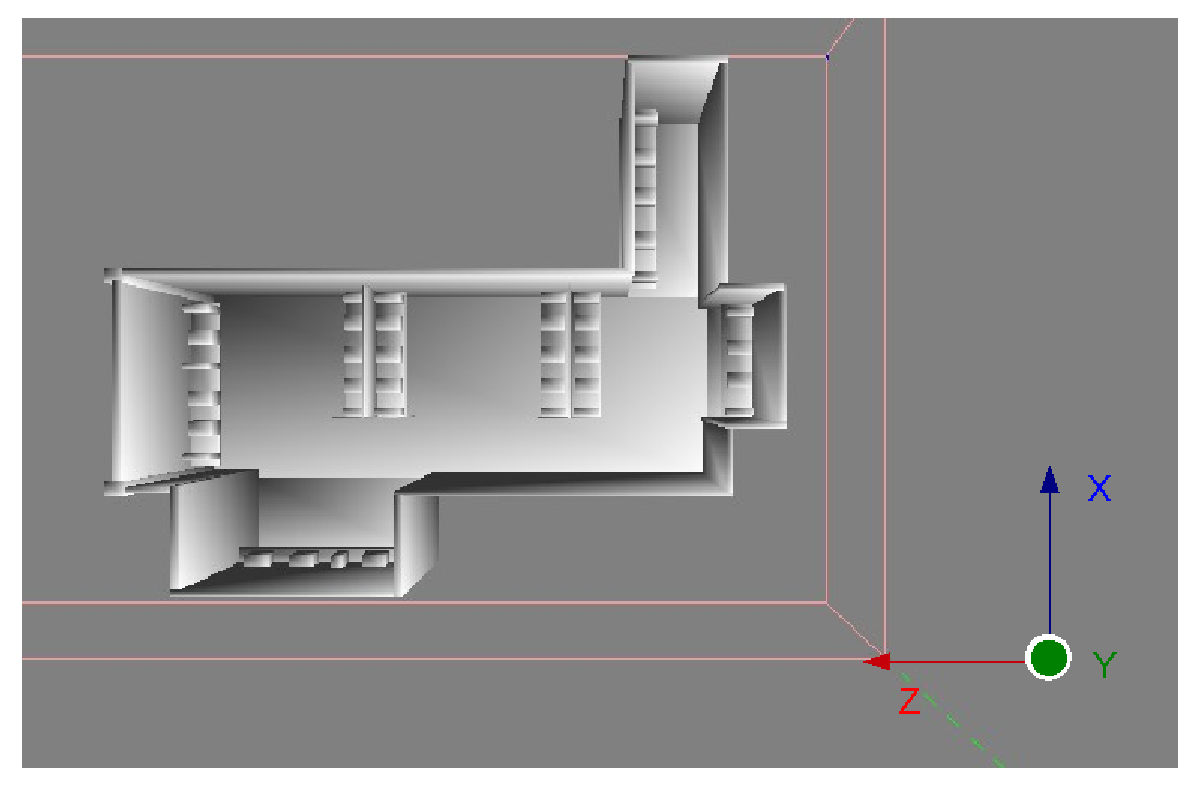
\includegraphics[scale = 0.4]{ambiente}
%	\caption{Visão topo em pespectiva do ambiente construído através da interface.}
%	\label{fg:ambiente}
%\end{figure}

%antenas e fontes
Depois de ambiente ter sido montado, surguiu a necessidade de introduzir a antena. Como a que foi usada na medição tinha uma forma complicada para modelagem, foi necessário criar uma que além de representar, funcionasse de forma semelhante com a real. Após fazer uma análise, se percebeu que a antena usada  durante as medições funcionava como um dipolo. Assim, alguns testes foram realizados desejando encontrar uma representação aceitável para o propósito.\\

Para todos os modelos de antenas criados, foi ultizada uma fonte de tensão de trêm de pulsos normalizado(Equação~\ref{eq:trem}), Figura~\ref{fg:tensao}, onde através da transforma de Fourier, pode-se observar se a mesma estava trabalhando na banda adequada (a banda de trabalho da antena real é de $700MHz$-$900MHz$). O resultado obtido foi o ilustrado na Figura~\ref{fg:f_fonte}.\\

\begin{equation}\label{eq:trem}
	\Gamma = \frac{Z_{L} - Z_{S}}{Z_{L} + Z_{S}}
\end{equation}

\begin{figure}[ht!]
	\begin{center}
		\subfigure[Gráfico da fonte(trêm de pulsos) no tempo.]{\label{fg:tensao}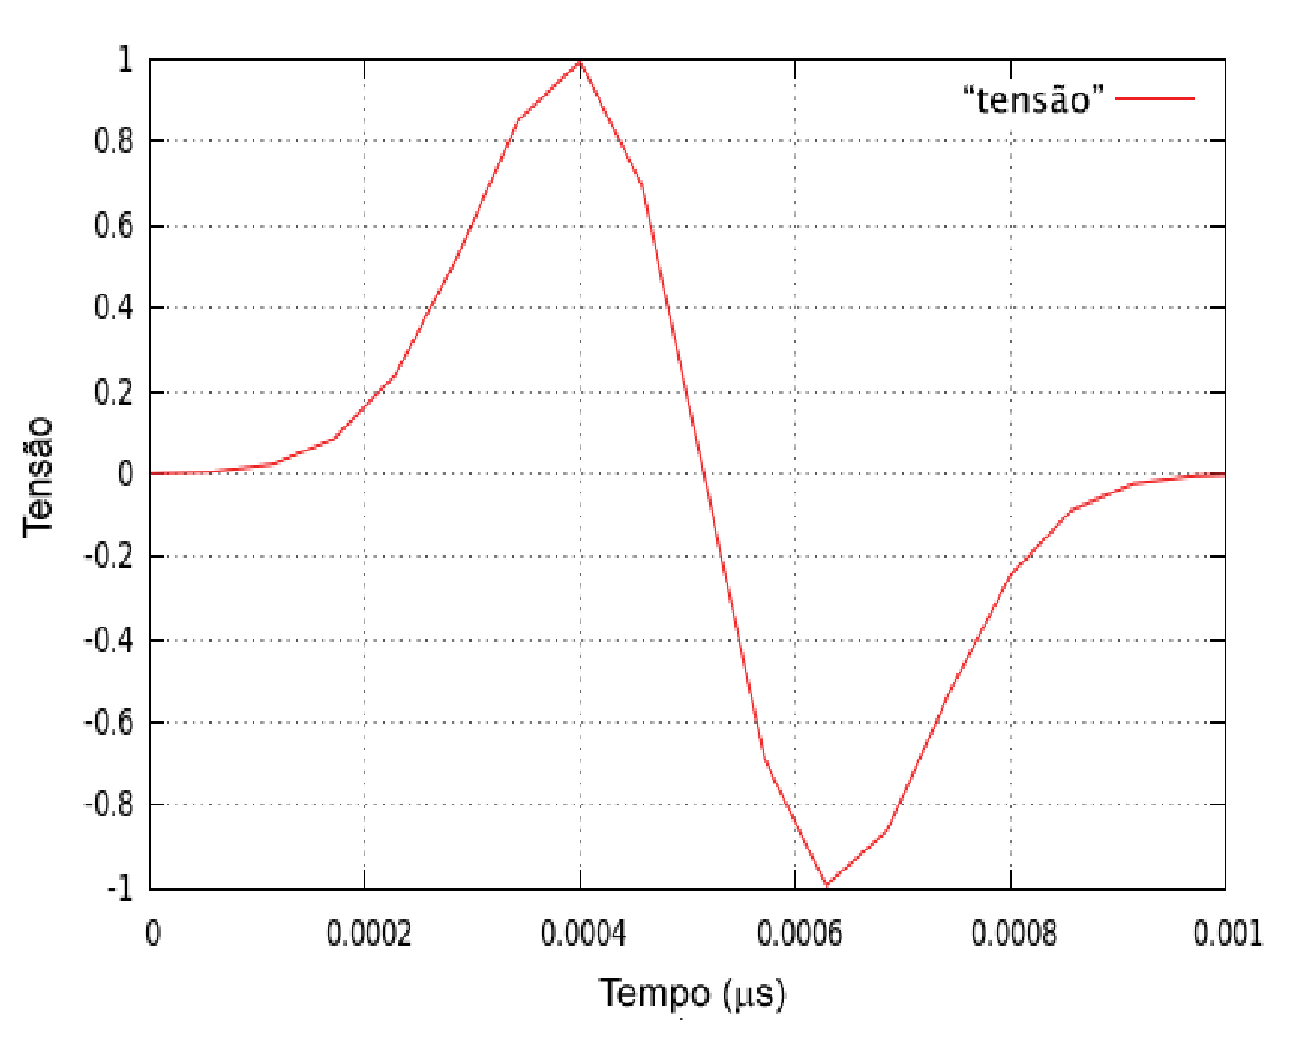
\includegraphics[scale=0.3]{tensao}}
\qquad
		\subfigure[Gráfico da transformada de Fourier da fonte.]{\label{fg:f_fonte}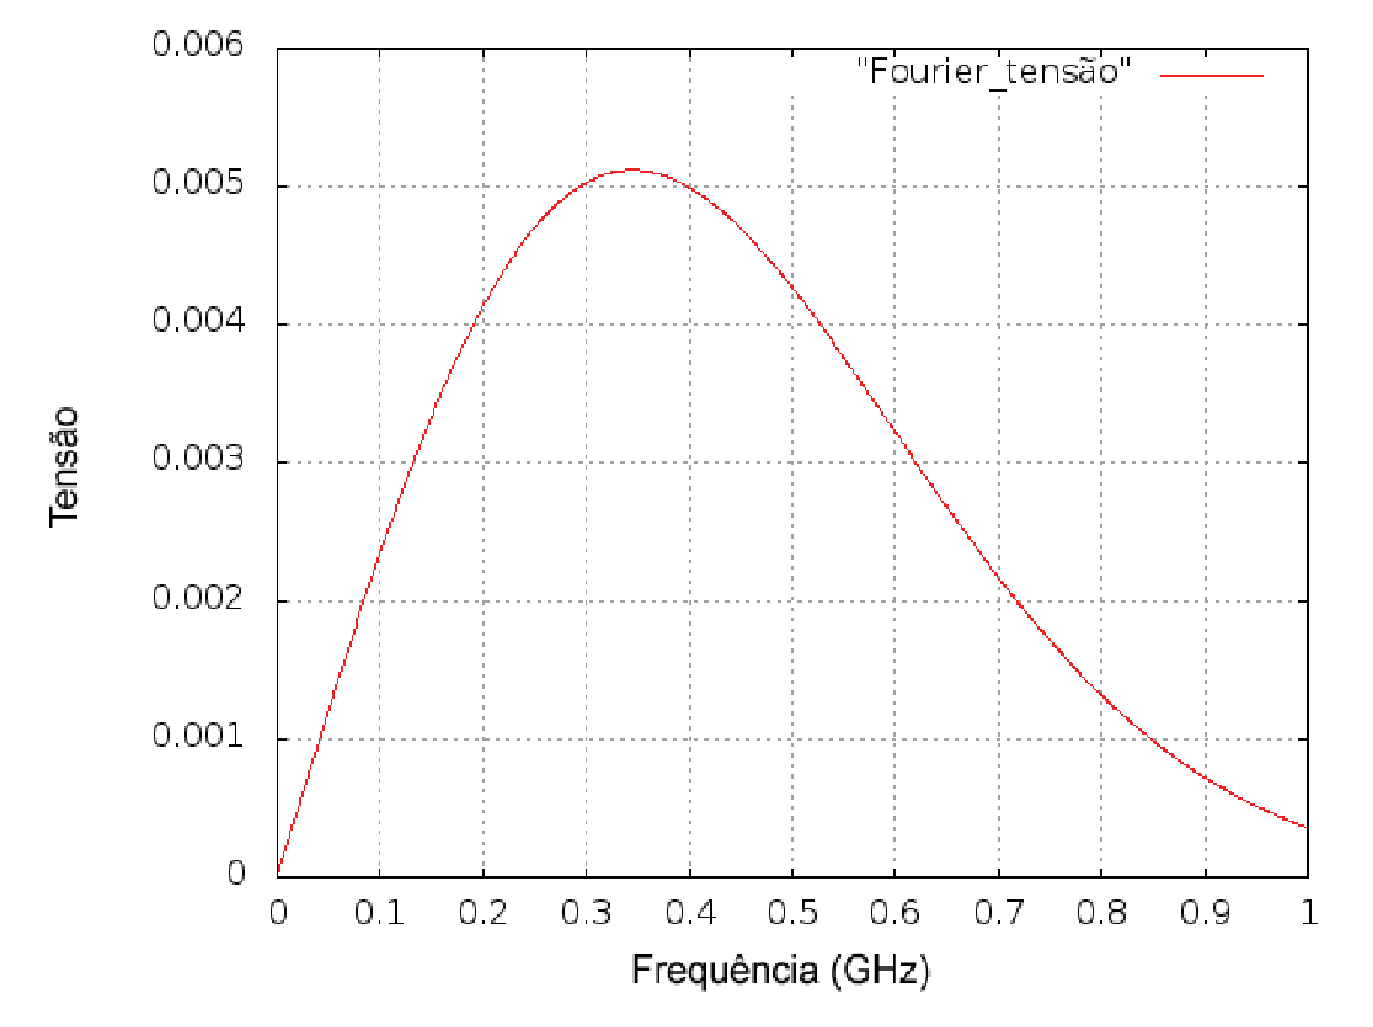
\includegraphics[scale=0.3]{f_fonte}}
	\end{center}
	\caption{Fonte de tensão usada nas antenas modeladas.}
	\label{fg:fontes}
\end{figure}

A primeira antena teste feita foi a mostrada no diagrama da Figura~\ref{fg:antena_normal}, juntamente com sua representação no LANE-SAGS(Figura~\ref{fg:antena_normal_sags}). Os blocos do seu diagrama tem as mesmas dimensões, assim como as hastes. Ela foi testada colocando a fonte entre as hastes, medindo a corrente na haste da esquerda e a tensão na mesma posição da fonte. \\

\begin{figure}[ht!]
	\begin{center}
		\subfigure[Diagrama da primeira antena dipolo criada.]{\label{fg:antena_normal}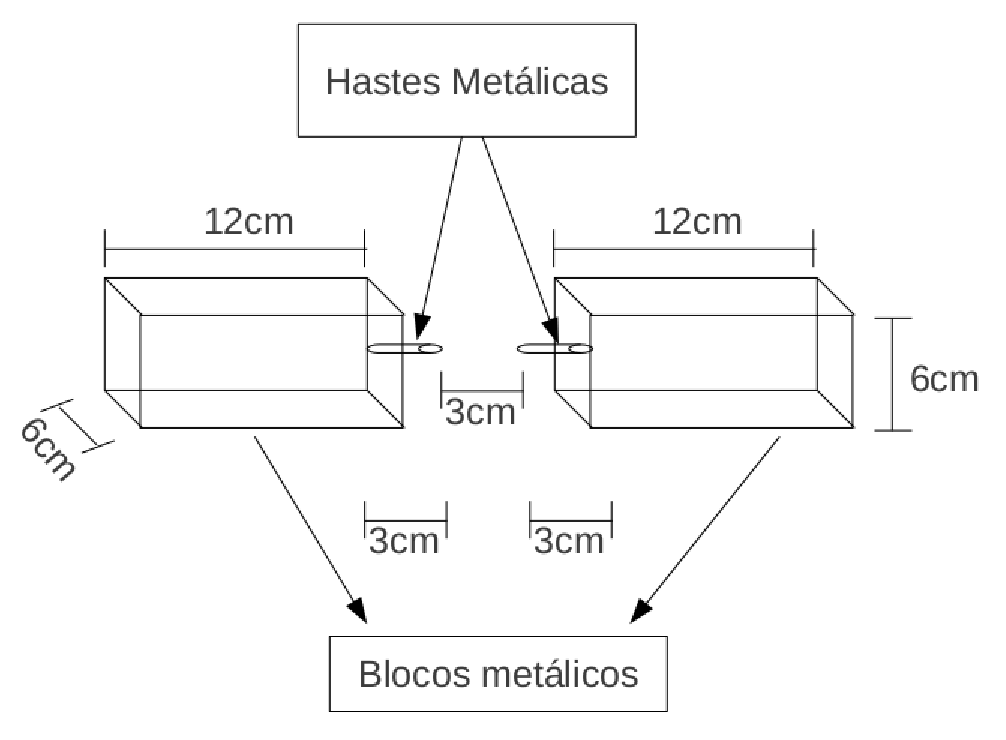
\includegraphics[scale=0.25]{antena_normal}}
\qquad
		\subfigure[Visualização da primeira antena no simulador LANE-SAGS.]{\label{fg:antena_normal_sags}\includegraphics[scale=0.25]{antena_normal_sags}}
	\end{center}
	\caption{Antena dipolo normal.}
	\label{fg:antena_normal_m}
\end{figure}

Com os dados de tensão e corrente, foi calculado o coeficiente de reflexão dessa antena através da fórmula mostrada na Equação~\ref{eq:impedancia}. Por meio dele pode-se computar a perda de retorno, Figura~\ref{fg:pr_01}, associada a essa antena(Equação~\ref{eq:pr}). Como pode-se observar na figura, essa antena trabalhando abaixo de $-10dB$ em uma faixa diferente da desejada($700MHz-900MHz$). Portanto, suas dimensões e parâmentros necessitaram ser modificados.\\

\begin{figure}[ht!]
	\centering
	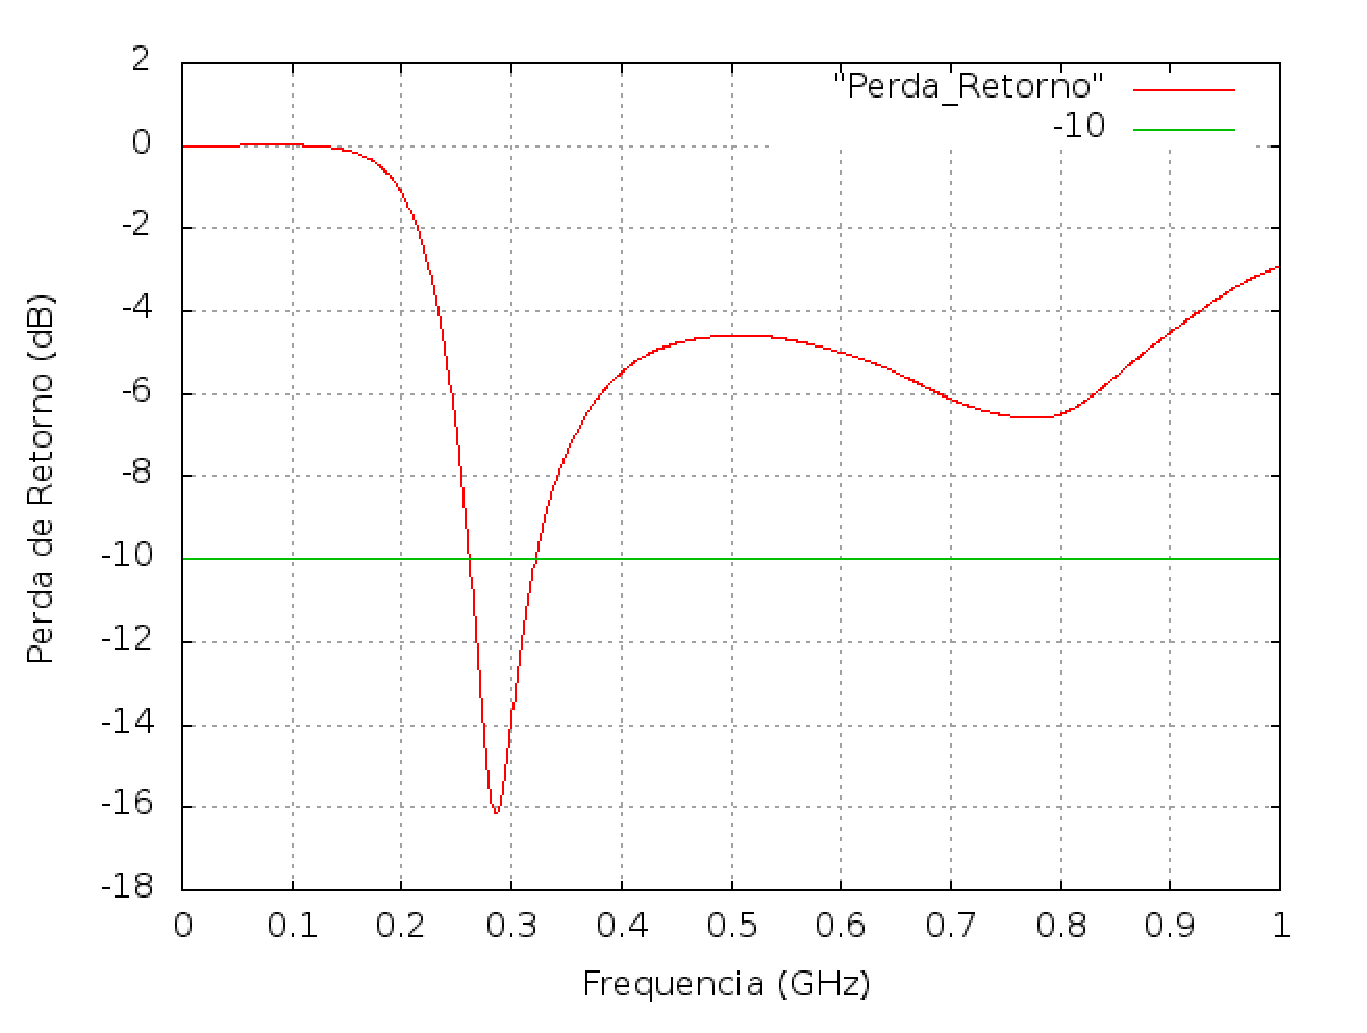
\includegraphics[scale = 0.5]{pr_01}
	\caption{Perda de retorno da antena dipolo normal(primeira antena modelada).}
	\label{fg:pr_01}
\end{figure}

\begin{equation}\label{eq:impedancia}
	\Gamma = \frac{Z_{L} - Z_{S}}{Z_{L} + Z_{S}}
\end{equation}
	Onde: $Z_{S}$ é a impedãncia de entrada($50 ohm$) e $Z_{L}$ representa a impedância relacionada a carga(calculada ponto a ponto com dados de tensão pela corrente coletados).
\begin{equation}\label{eq:pr}
	RL(dB) = -20log_{10} |\Gamma|
\end{equation}

Após alguns teste, verificou-se que a diminuição na dimensão dessa antena afetava de forma positiva o resultado da perda de retorno, porém tinhamos um impasse ligado ao fato do tamanho do \textit{delta}(que diminuiria de forma proporcional). Portanto se a diminuiçao fosse grande, ficaria improvavel a simulação desse ambiente, mesmo ele sendo pequeno, pelo seu custo computacional. Surgiu então a idéia do uso de um capacitor(com capacitância igual a $3,7\times10^{-5} farad$) aclopado um dos blocos métalicos, através de sua impedância simularia a diminuição sem precisarmos de fato mexer tanto nas dimensões da antena.\\

A configuração da antena adaptada esta ilustrada no diagrama da Figura~\ref{fg:antena_final}. A Figura~\ref{fg:antena_final_sags} mostra ela no LANE-SAGS. Os cálculos feitos para antena anterior foram refeitos, como resultado obteve-se a perda de retorno desejada mostrada na Figura~\ref{fg:pr_2}, que faz também uma comparação com a obtida anteriormente.\\

\begin{figure}[ht!]
	\centering
	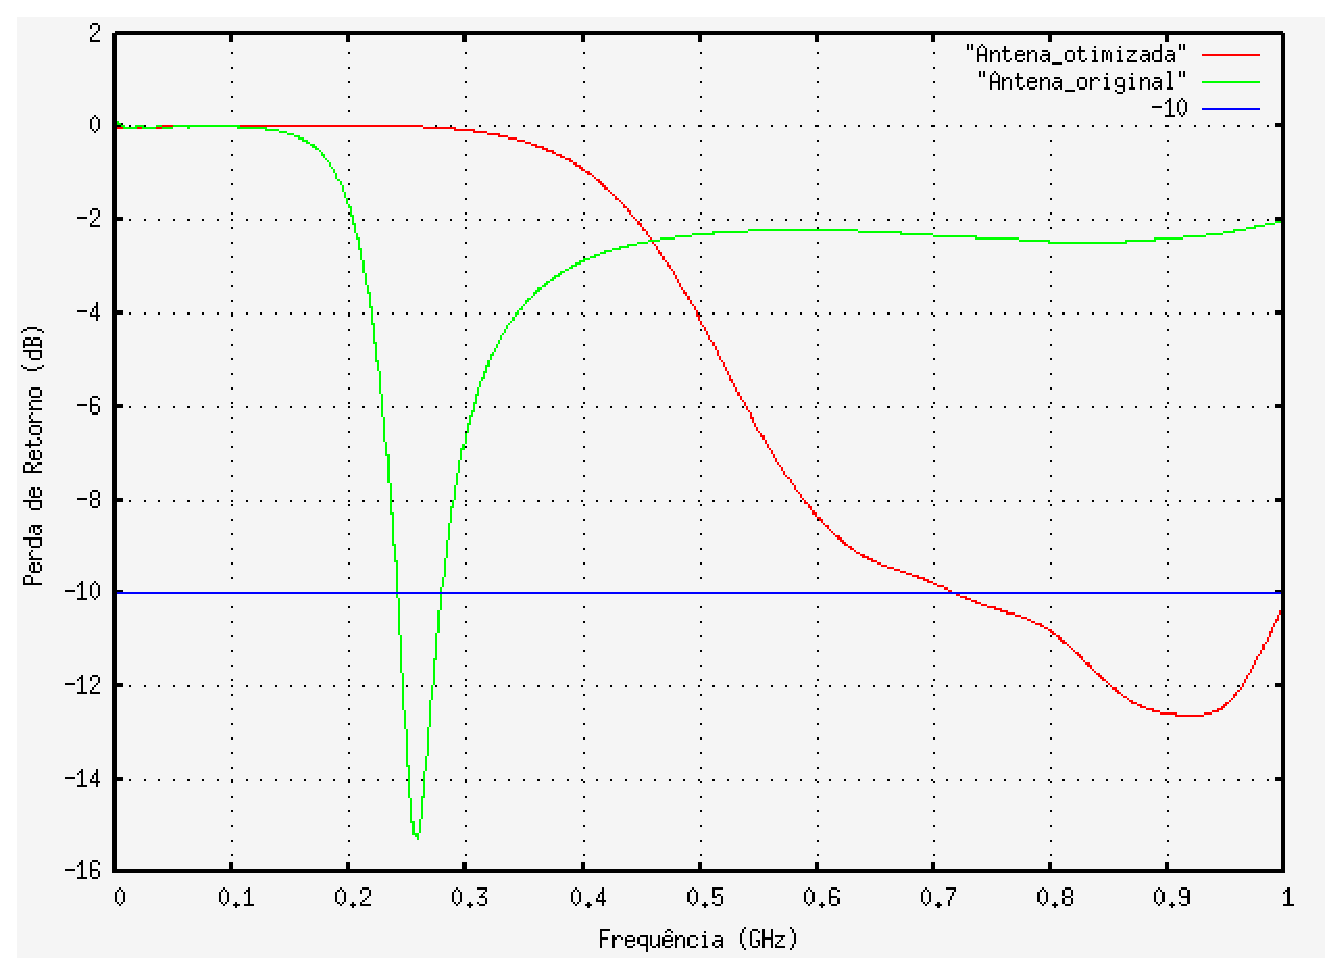
\includegraphics[scale = 0.5]{pr_2}
	\caption{Comparação entre as perdas de retorno da antena otimizada(adaptada) e normal(original).}
	\label{fg:pr_2}
\end{figure}

\begin{figure}[ht!]
	\begin{center}
		\subfigure[Diagrama da antena dipolo adaptada.]{\label{fg:antena_final}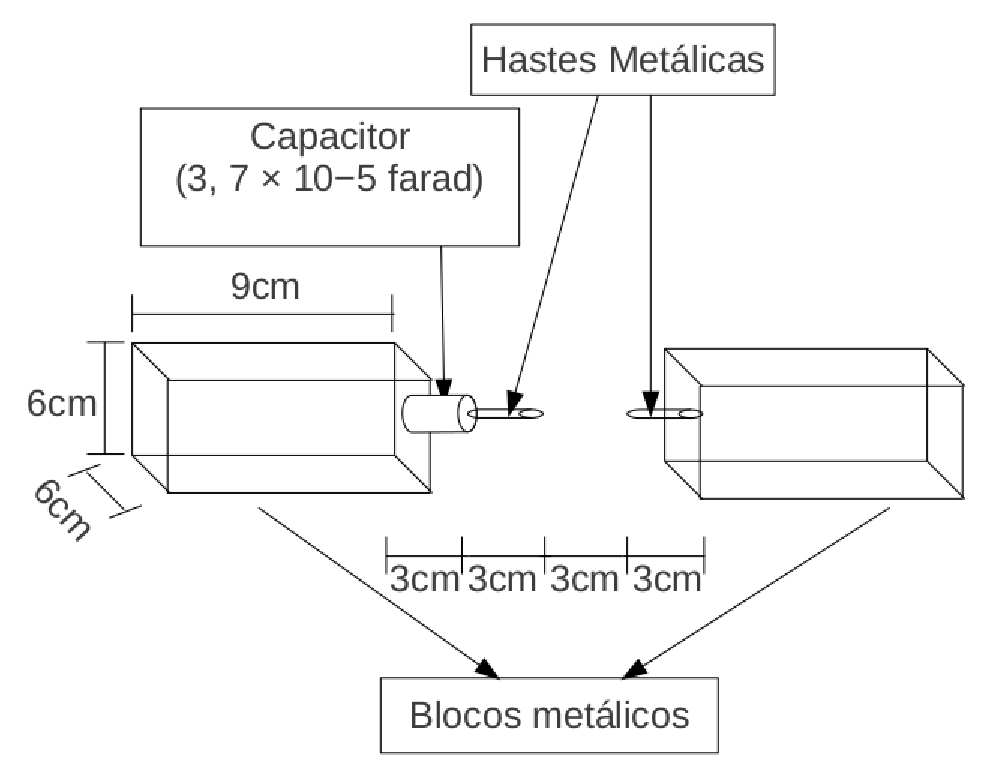
\includegraphics[scale=0.25]{antena_final}}
\qquad
		\subfigure[Visualização da antena adaptada no simulador LANE-SAGS.]{\label{fg:antena_final_sags}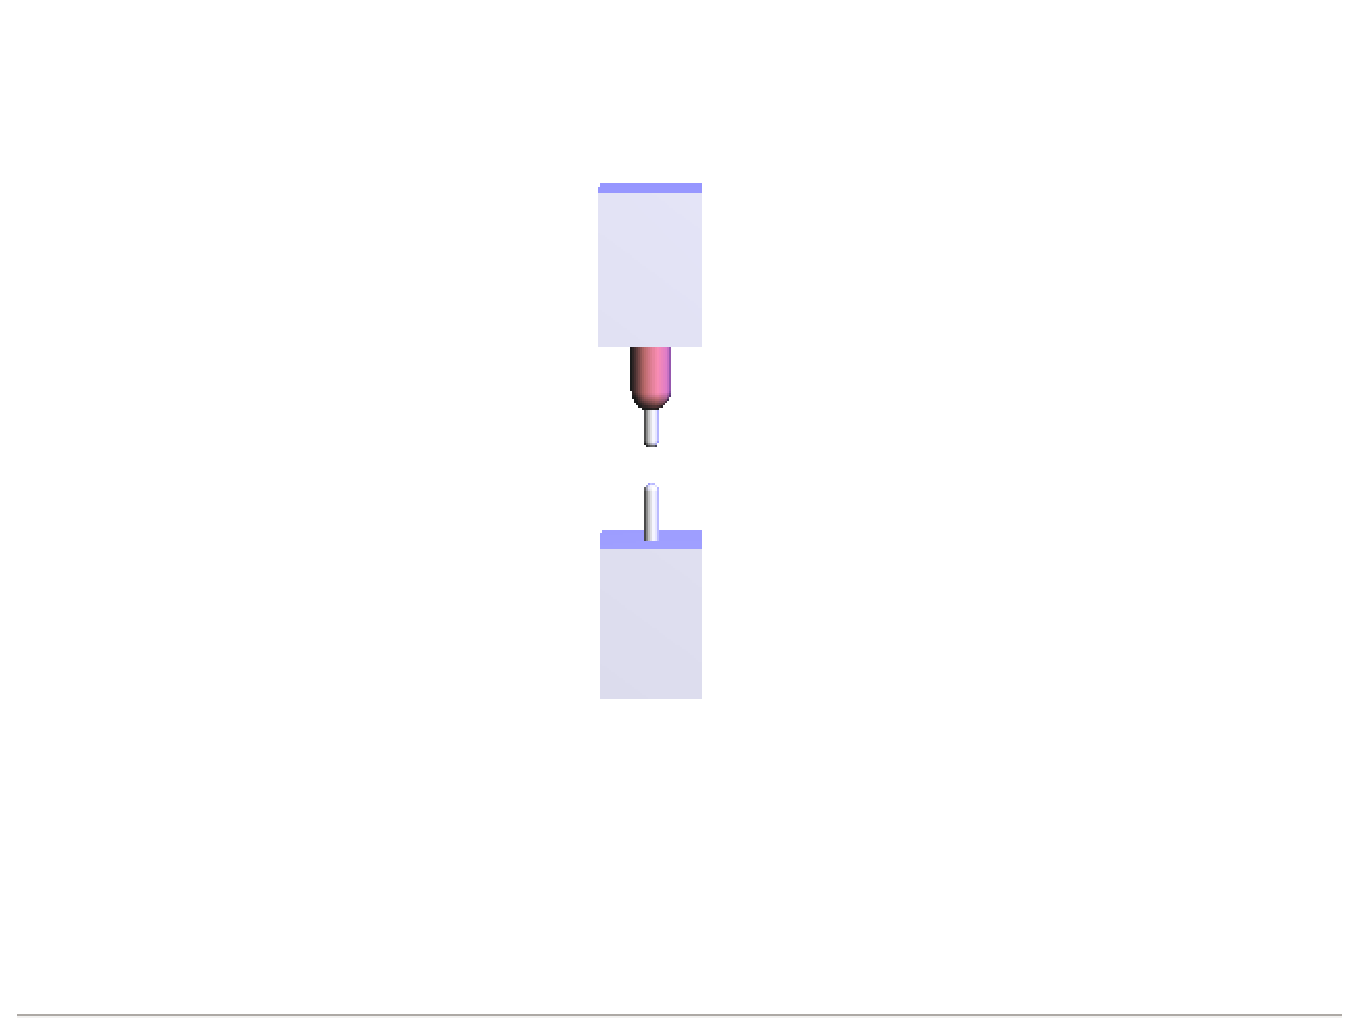
\includegraphics[scale=0.25]{antena_final_sags}}
	\end{center}
	\caption{Antena dipolo adaptada.}
	\label{fg:antena_apatada}
\end{figure}

%resultados
\subsection{Caso 01}
O caso 01 referesse a introdução da antena modelada na posição $T1$ da Figura~\ref{fg:planta_baixa}. Ela foi posicionada a uma altura de $1,5m$ do piso. Com isso foi feita a simulação obeteve-se além da tensão calculada no ponto R(que tem a mesma altura do ponto $T1$) do cenário modelado, a tensão entre as hastes da antena. Esse sinais estão mostrados nas Figuras~\ref{fg:t_out} e \ref{fg:t_in}.

\begin{figure}[ht!]
	\begin{center}
		\subfigure[Gráfico da tensão no Ponto R.]{\label{fg:t_out}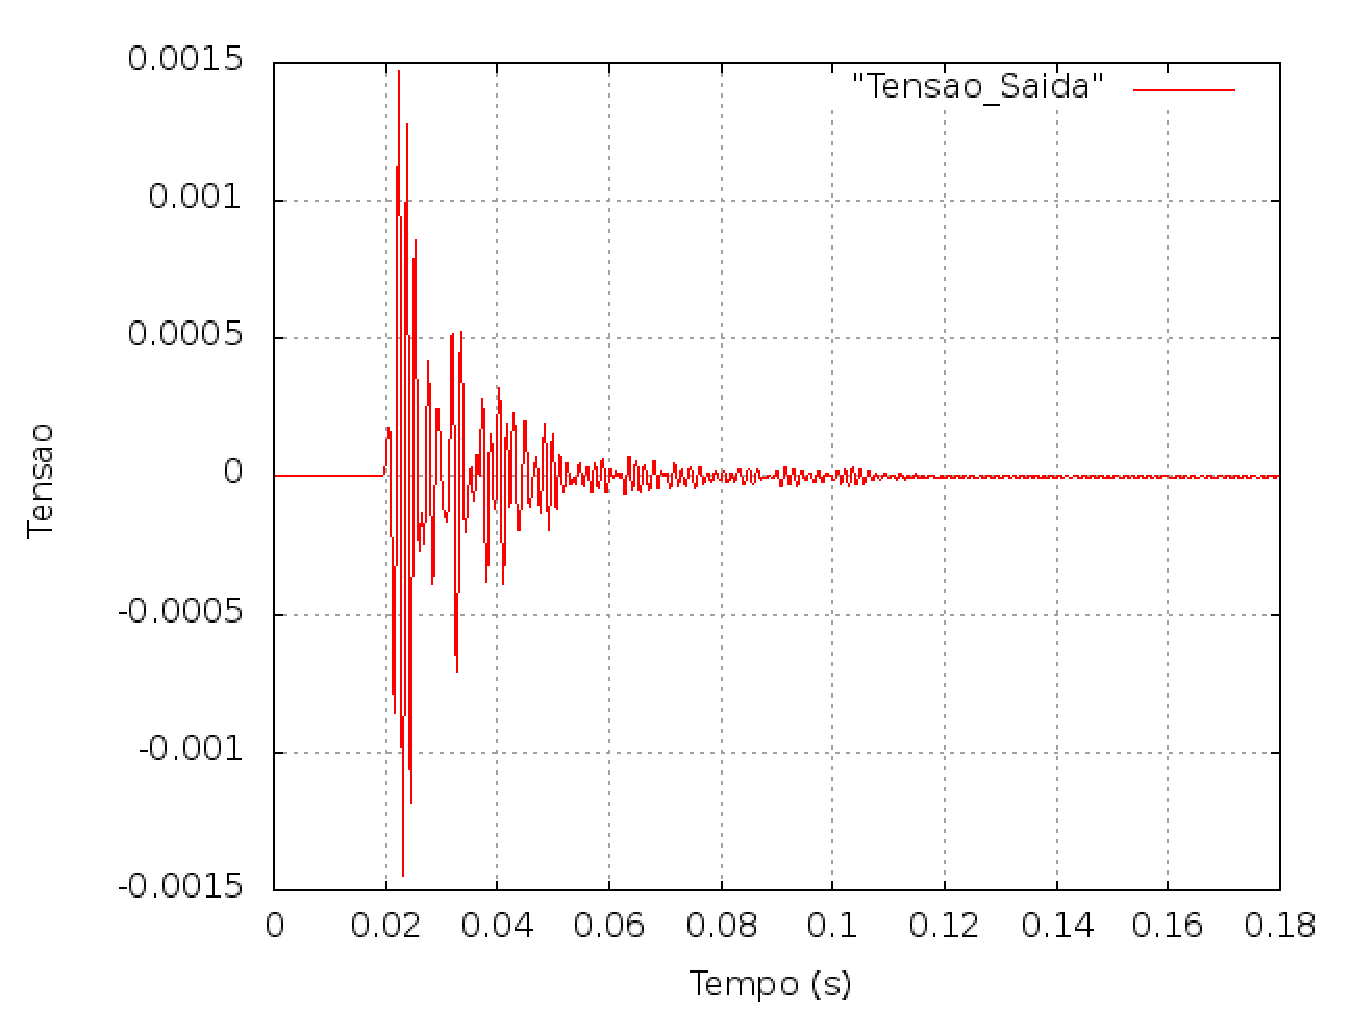
\includegraphics[scale=0.25]{t_out}}
\qquad
		\subfigure[Gráfico da tensão no Ponto $T1$(entre as hastes da antena).]{\label{fg:t_in}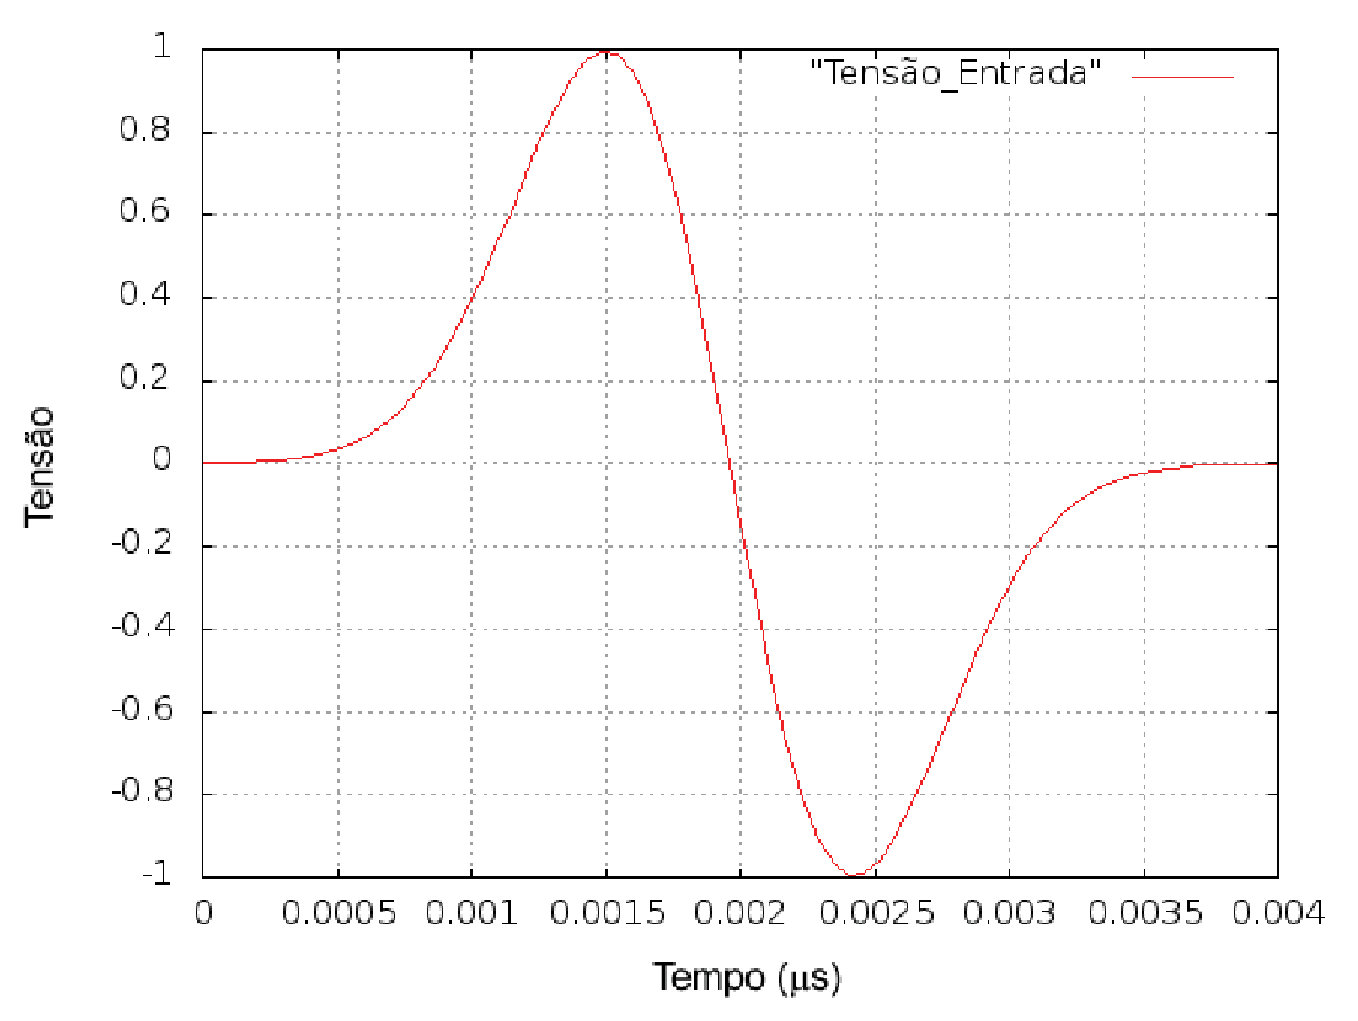
\includegraphics[scale=0.25]{t_in}}
	\end{center}
	\caption{Tensões obtidas pela simulação.}
	\label{fg:tensoes}
\end{figure}

Por meio desses dados de entrada e saída, desejava-se calcular o perfil de potência e retardo do canal, $ P_h(\varsigma)$, desse ambiente virtual simulado, para comparar com o medido. Todavia, para que isso fosse possível, era necessário ter a resposta impulsiva desse canal. A Figura~\ref{fg:hf} mostra o processo de obetenção da resposta em frequência.\\
\begin{figure}[ht!]
	\centering
	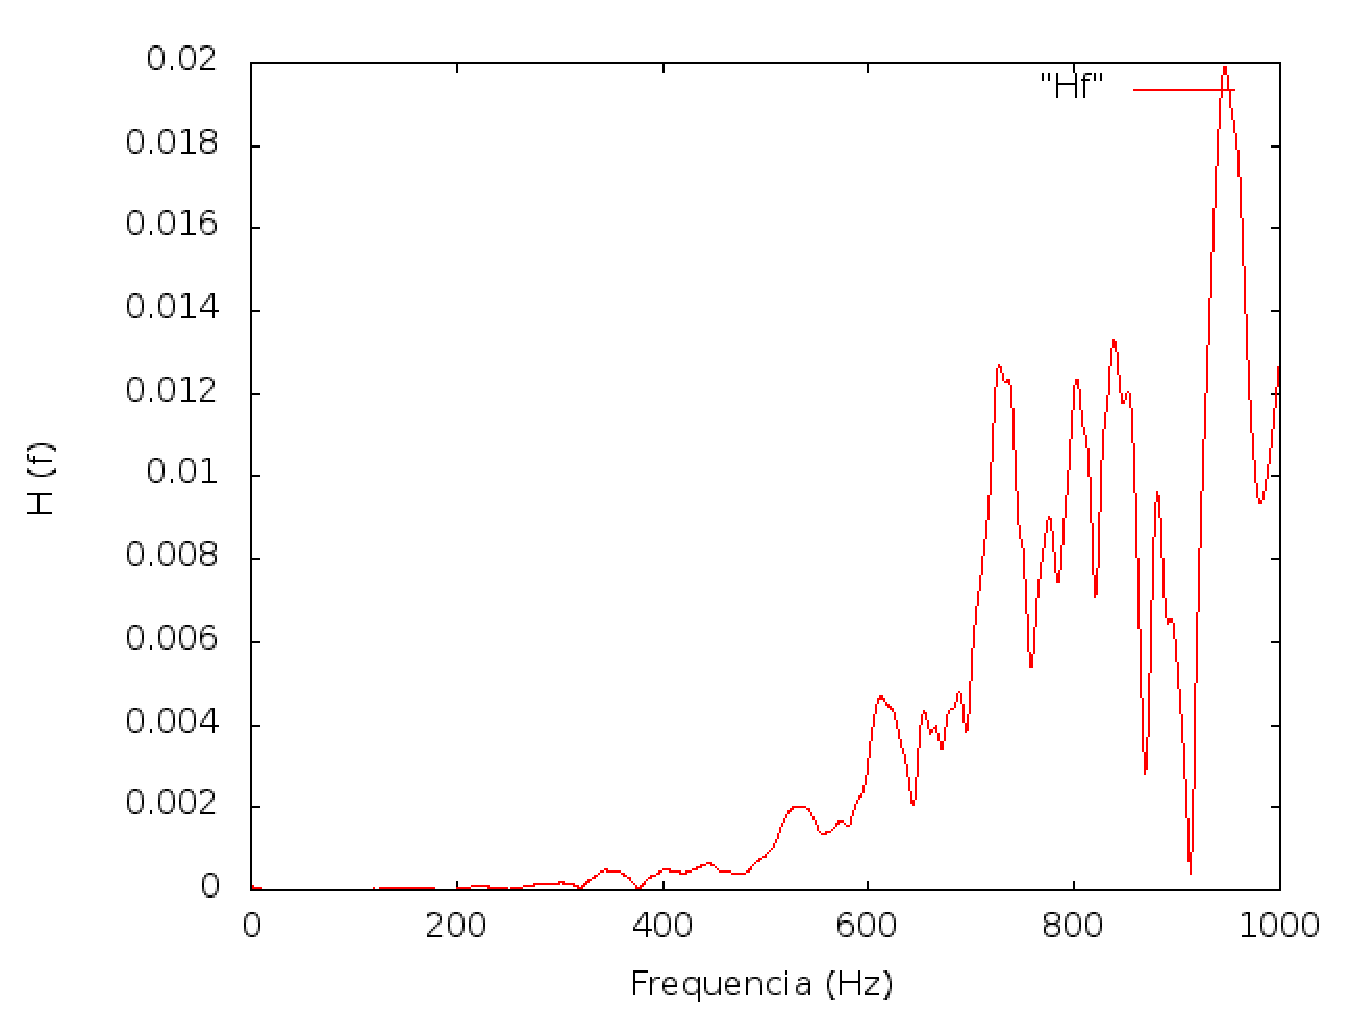
\includegraphics[scale = 0.5]{hf}
	\caption{Diagrama de bloco ilustrando a operação linear de obtenção da função de transferência $Hf(f)$.}
	\label{fg:hf}
\end{figure}

Logo, as tensões de entrada(referente ao ponto $T1$) e saída (referente ao ponto $R$), usando a transformada de Fourier, foram lanchadas para o domínio da frequência e então divididas ponto a ponto. Com isso se obeteve a resposta em frequência, $H( f )$. Usando a Equação~\ref{eq:ant_f},referente a anti-transformada de Fourier, se obter a resposta impulsiva desse canal.\\


Através da Equação~\ref{eq:pp} foi possível fazer a comparação com os dados da medição. A Figura~\ref{fg:ms} mostra essa comparação.

\begin{equation}\label{eq:ant_f}
	h(\varsigma) = \mathcal{F^{-1}}{H(f)}
\end{equation}

\begin{figure}[ht!]
	\centering
	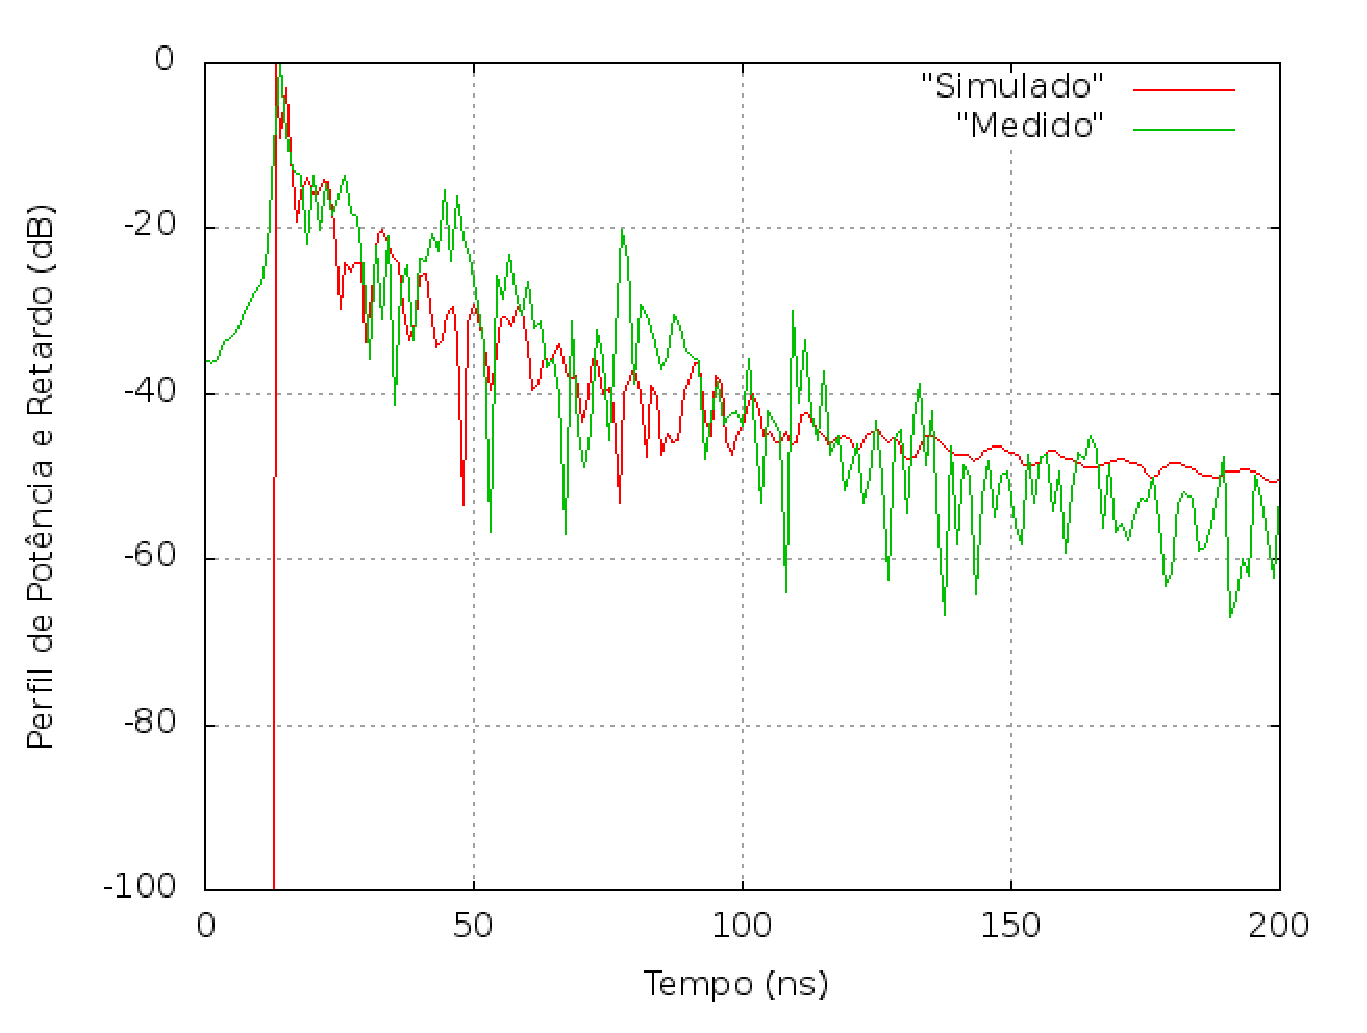
\includegraphics[scale = 0.5]{ms}
	\caption{Comparação entre medição e simulação.}
	\label{fg:ms}
\end{figure}


\chapter{Considerações Finais}
%%Nesse trabalho foi desenvolvido um software de modelagem 3D que permite construir ambientes virtuais baseados nas características dos reais. Ele se utiliza das técnicas de modelagem mais usadas no mercado, além de também utilizar da teoria de grafo de cena. Possibilitando que o cenário nele desenvolvido simule a propagação de ondas eletromagnéticas usando a método FDTD.\\

%Um estudo de caso foi realisado, obtendo um resultado satisfatório que comprovou que tanto a modelagem quanto a conexão com o simulador LANE-SAGS funcionaram de forma desejada. Assim, mostrando que a interface desenvolvida cumpriu com os requisitos prospostos para esse projeto.

%\subsection{Trabalhos Futuros}
%Como prosseguimento natural desse trabalho, pretende-se:
%\begin{itemize}
%	\item{Melhorar a classe de conexão irrlicht-qt}
%	\item{Adicionar novos objetos ao conjunto já existentes.}
%	\item{Possibilitar o agrupamento e desagrupamento de objetos no ambiente virtual.}
%	\item{Possibilitar a imersão nos cenários criados através de uma re-estruturação do software.}

%\end{itemize}

Ainda estou terminando.


\renewcommand\bibname{Referências Bibliográficas}
%\bibliographystyle{abnt-num} % Estilo para gerar referncias em conformidade com
                          % as normas brasileiras
\bibliographystyle{./public/IEEEtran}
\bibliography{tccMocbel}

\clearpage
%\appendix

%% -- aqui termina o TCC
\end{document}
